\documentclass[sigconf,10pt]{acmart}

%\usepackage[•]{•}{microtype}

\usepackage{booktabs} % For formal tables
%\usepackage[subtle]{savetrees}
%\settopmatter{printacmref=true}
% Copyright
%\setcopyright{none}
%\setcopyright{acmcopyright}
%\setcopyright{acmlicensed}
%\setcopyright{rightsretained}
%\setcopyright{usgov}
%\setcopyright{usgovmixed}
%\setcopyright{cagov}
%\setcopyright{cagovmixed}
\newcommand{\minihead}[1]{{\vspace{.5em}\noindent\textbf{#1} }}
\newcommand{\red}[1]{{\color{black}#1}}
\newcommand{\mvar}{\red{d}}
\newcommand{\dvar}{\red{n}}

\newcommand\code[1]{\lstinline$#1$}

%%%%%%%%%%%%
\renewcommand\paragraph{\@startsection{paragraph}{4}{\z@}%
                                    {0.5ex \@plus 0.5ex \@minus .2ex}%
                                    {-0.5em}%
                                    {\normalfont\normalsize\bfseries}}
\usepackage[labelfont=bf]{caption}
\setlength{\intextsep}{5pt plus 1.0pt minus 2.0pt}
\setlength{\abovedisplayskip}{1pt}
\setlength{\belowdisplayskip}{1pt}
%\usepackage[small,compact]{titlesec}

%\newenvironment{denseitemize}{
%\begin{itemize}[topsep=2pt, partopsep=0pt, leftmargin=1.5em]
%  \setlength{\itemsep}{4pt}
%  \setlength{\parskip}{0pt}
%  \setlength{\parsep}{0pt}
%}{\end{itemize}}
%
%\newenvironment{denseenum}{
%\begin{enumerate}[topsep=2pt, partopsep=0pt, leftmargin=1.5em]
%  \setlength{\itemsep}{4pt}
%  \setlength{\parskip}{0pt}
%  \setlength{\parsep}{0pt}
%}{\end{enumerate}}

%\newcommand{\subparagraph}{}
%\usepackage[small,compact]{titlesec}
%\renewcommand{\paragraph}[1]{\vspace{1mm}\noindent \textbf{#1}}
%\usepackage[labelfont=bf,skip=2pt,belowskip=2pt]{caption}
%%%%%%%%%%%

\usepackage{enumitem}


\usepackage{algorithm}
\usepackage[noend]{algpseudocode}
\algdef{SE}[DOWHILE]{Do}{doWhile}{\algorithmicdo}[1]{\algorithmicwhile\ #1}%

\theoremstyle{problem}
\newtheorem{problem}{Problem}[section]



% DOI
%\acmDOI{10.475/123_4}

% ISBN
%\acmISBN{123-4567-24-567/08/06}

%Conference
\acmConference[DEEM'19]{DEEM}{June 2019}{Amsterdam, The Netherlands}
\acmYear{2019}
\acmPrice{15.00}
\acmDOI{10.1145/1122445.1122456}
\acmISBN{978-1-4503-9999-9/18/06}


%Conference


\begin{document}
\title{DROP: A Workload-Aware Optimizer for Dimensionality Reduction}


\author{Sahaana Suri, Peter Bailis}
\affiliation{
  \institution{Stanford University}
}

\renewcommand{\shortauthors}{S. Suri and P. Bailis}



\begin{abstract}
Dimensionality reduction (DR) is a critical step in scaling machine learning pipelines. Principal component analysis (PCA) is a standard DR tool, but classic methods for computing PCA over a full dataset can be computationally expensive: $O(dn^2 + n^3)$ for an $n$-dimensional dataset of $d$ points. 
As a result, theoretical work has studied the effectiveness of iterative, stochastic PCA methods that operate over data samples. 
However, termination conditions for stochastic PCA either execute for a predetermined number of iterations, or until convergence of the solution, frequently sampling too many or too few datapoints for end-to-end runtime improvements. We show how accounting for downstream analytics operations during DR via PCA allows stochastic methods to efficiently terminate after operating over small (e.g., 1\%) subsamples of input data, reducing whole workload runtime. 
Leveraging this, we propose DROP, a DR optimizer that enables speedups of up to \red{$5\times$} over \red{Singular-Value-Decomposition-based} PCA techniques, and exceeds conventional approaches like FFT and PAA by up to \red{$16\times$} in end-to-end workloads.
\end{abstract}


\begin{CCSXML}
<ccs2012>
<concept>
<concept_id>10010147.10010257.10010258.10010262.10010277</concept_id>
<concept_desc>Computing methodologies~Transfer learning</concept_desc>
<concept_significance>500</concept_significance>
</concept>
<concept>
<concept_id>10002951.10003227.10003351</concept_id>
<concept_desc>Information systems~Data mining</concept_desc>
<concept_significance>300</concept_significance>
</concept>
</ccs2012>
\end{CCSXML}

\maketitle

%\section*{abstract}
Dimensionality reduction is a critical step in scaling machine learning pipelines. Principal component analysis (PCA) is a standard tool for dimensionality reduction, but performing PCA over a full dataset can be prohibitively expensive. 
As a result, theoretical work has studied the effectiveness of iterative, stochastic PCA methods that operate over data samples. 
However, termination conditions for stochastic PCA either execute for a predetermined number of iterations, or until convergence of the solution, frequently sampling too many or too few datapoints for end-to-end runtime improvements. We show how accounting for downstream analytics operations during DR via PCA allows stochastic methods to efficiently terminate after operating over small (e.g., 1\%) subsamples of input data, reducing whole workload runtime. 
Leveraging this, we propose a DR optimizer that enables speedups of up to \red{$5\times$} over \red{Singular-Value-Decomposition-based} PCA techniques, and exceeds conventional approaches like FFT and PAA by up to \red{$16\times$} in end-to-end workloads.




%This enables end-to-end optimization over both dimensionality reduction and analytics tasks.
%By combining techniques spanning progressive sampling, approximate query processing, and cost-based optimization, we propose a dimensionality reduction optimizer that enables speedups of up to \red{$5\times$} over \red{Singular-Value-Decomposition-based} PCA techniques, and achieves parity with or exceeds conventional approaches like FFT and PAA by up to \red{$16\times$} in end-to-end workloads.

%As time series analytics workloads grow, we see an increase in time series tools and DB stuff to enable more efficient TS analytics routines. 
%In order to facilitate this, indexing of time series is important---and DR plays a critical step in this.





%DROP uses the key insight that structured data such as time series can be sufficiently characterized by a small subset of data, which permits aggressive sampling during dimensionality reduction.  
%Sampling allows DROP to uncover high quality low-dimensional bases in runtime proportional to the dataset's intrinsic dimensionality---\textit{independent} of the actual dataset size.
%Additionally, DROP uses online progress estimation to predict DROP and downstream runtime costs, enabling a trade-off between degree of dimensionality reduction and pipeline runtime, and obviating the need for the intrinsic data dimension to be specified by the user. 
%At a high level, DROP progressively samples its input, computes a candidate transformation, and terminates once it finds a low dimensional representation of suitable size and quality quickly enough to not bottleneck downstream tasks. DROP provides speedups of up to $50\times$ over the na\"ive, SVD-based approach and $33\times$  in end-to-end analytics pipelines.
%A dataset's intrinsic dimensionality is also typically unknown a priori (i.e., to what extent a dataset can be compressed), a necessary parameter for dimensionality reduction via PCA.
%Further, based on downstream analytics tasks, it may be crucial to quickly return a result even if it is of dimension higher than the intrinsic dimension, but sufficient for the task at hand.
%To address these challenges, we present DROP, a new dynamic optimizer for high-dimensional analytics pipelines that efficiently computes high quality results (low-dimensional bases) via approximate PCA, without PCA's expensive runtime.
%dimensionality reduction optimizer that efficiently performs PCA in high-dimensional analytics pipelines.
%new dynamic optimizer that efficiently computes high quality results (i.e., low-dimensional basis) without the expensive runtime of PCA
%DROP reduces the cost of PCA over structured datasets, and automatically identifies a low dimensional data representation by taking the runtime of downstream analytics tasks into consideration.




%DROP enables downstream-operation-aware optimization via online progress estimation, trading-off degree of dimensionality reduction with the combined runtime of DROP and downstream analytics tasks. 

%In this paper, we revisit a now-classic study of time series dimensionality reduction operators and find that for a given quality constraint, Principal Component Analysis (PCA) uncovers representations that are over $2\times$ smaller than those obtained via alternative techniques favored in the time series literature. 


\section{Introduction}
\label{sec:intro}

Continued, rapid growth in high-dimensional data from automated data sources~\cite{plato,macrobase-cidr} poses a scalability challenge for machine learning (ML) pipelines.
Dimensionality reduction (DR) techniques can alleviate this scalability challenge~\cite{keogh-indexing,local-dr,decade,gemini}.
In exchange for a runtime cost ($R$), DR methods transform an $n$-dimensional dataset to a lower $k$-dimensional representation while preserving salient dataset features, allowing downstream analytics routines to terminate in runtime proportional to $k > n$, while preserving accuracy on downstream tasks (see Figure~\ref{fig:pipeline}).

Principal Component Analysis (PCA) is often the DR method of choice for practitioners with respect to transformation quality ($k$) for a target accuracy~\cite{jolbook}. However, na\"{i}ve implementations of PCA are data and workload-independent, and scale poorly with dimensionality, resulting in runtimes ($R$) that exceed the downstream runtime benefit of DR via PCA. Accordingly, practitioners often sacrifice quality for end-to-end runtime, and use alternative DR methods~\cite{keogh-study}. 

Sample-based, stochastic PCA algorithms~\cite{shamir,re-new} are a scalable alternative to classical PCA.
However, the amount of sampling required is highly data-dependent.
If we sample too many data points, then the runtime overhead of PCA in an end-to-end analytics workload could outweigh the statistical benefits.
If we fail to sample enough data points, then PCA could fail to deliver a sufficiently high-quality reduction and compromise the runtime and/or accuracy of downstream analytics.
This raises a critical question: can we develop a data and workload-dependent means of efficiently and accurately determining the sampling rate for stochastic PCA, such that we can obtain PCA's transformation quality while minimizing end-to-end workload runtime?

\begin{figure}
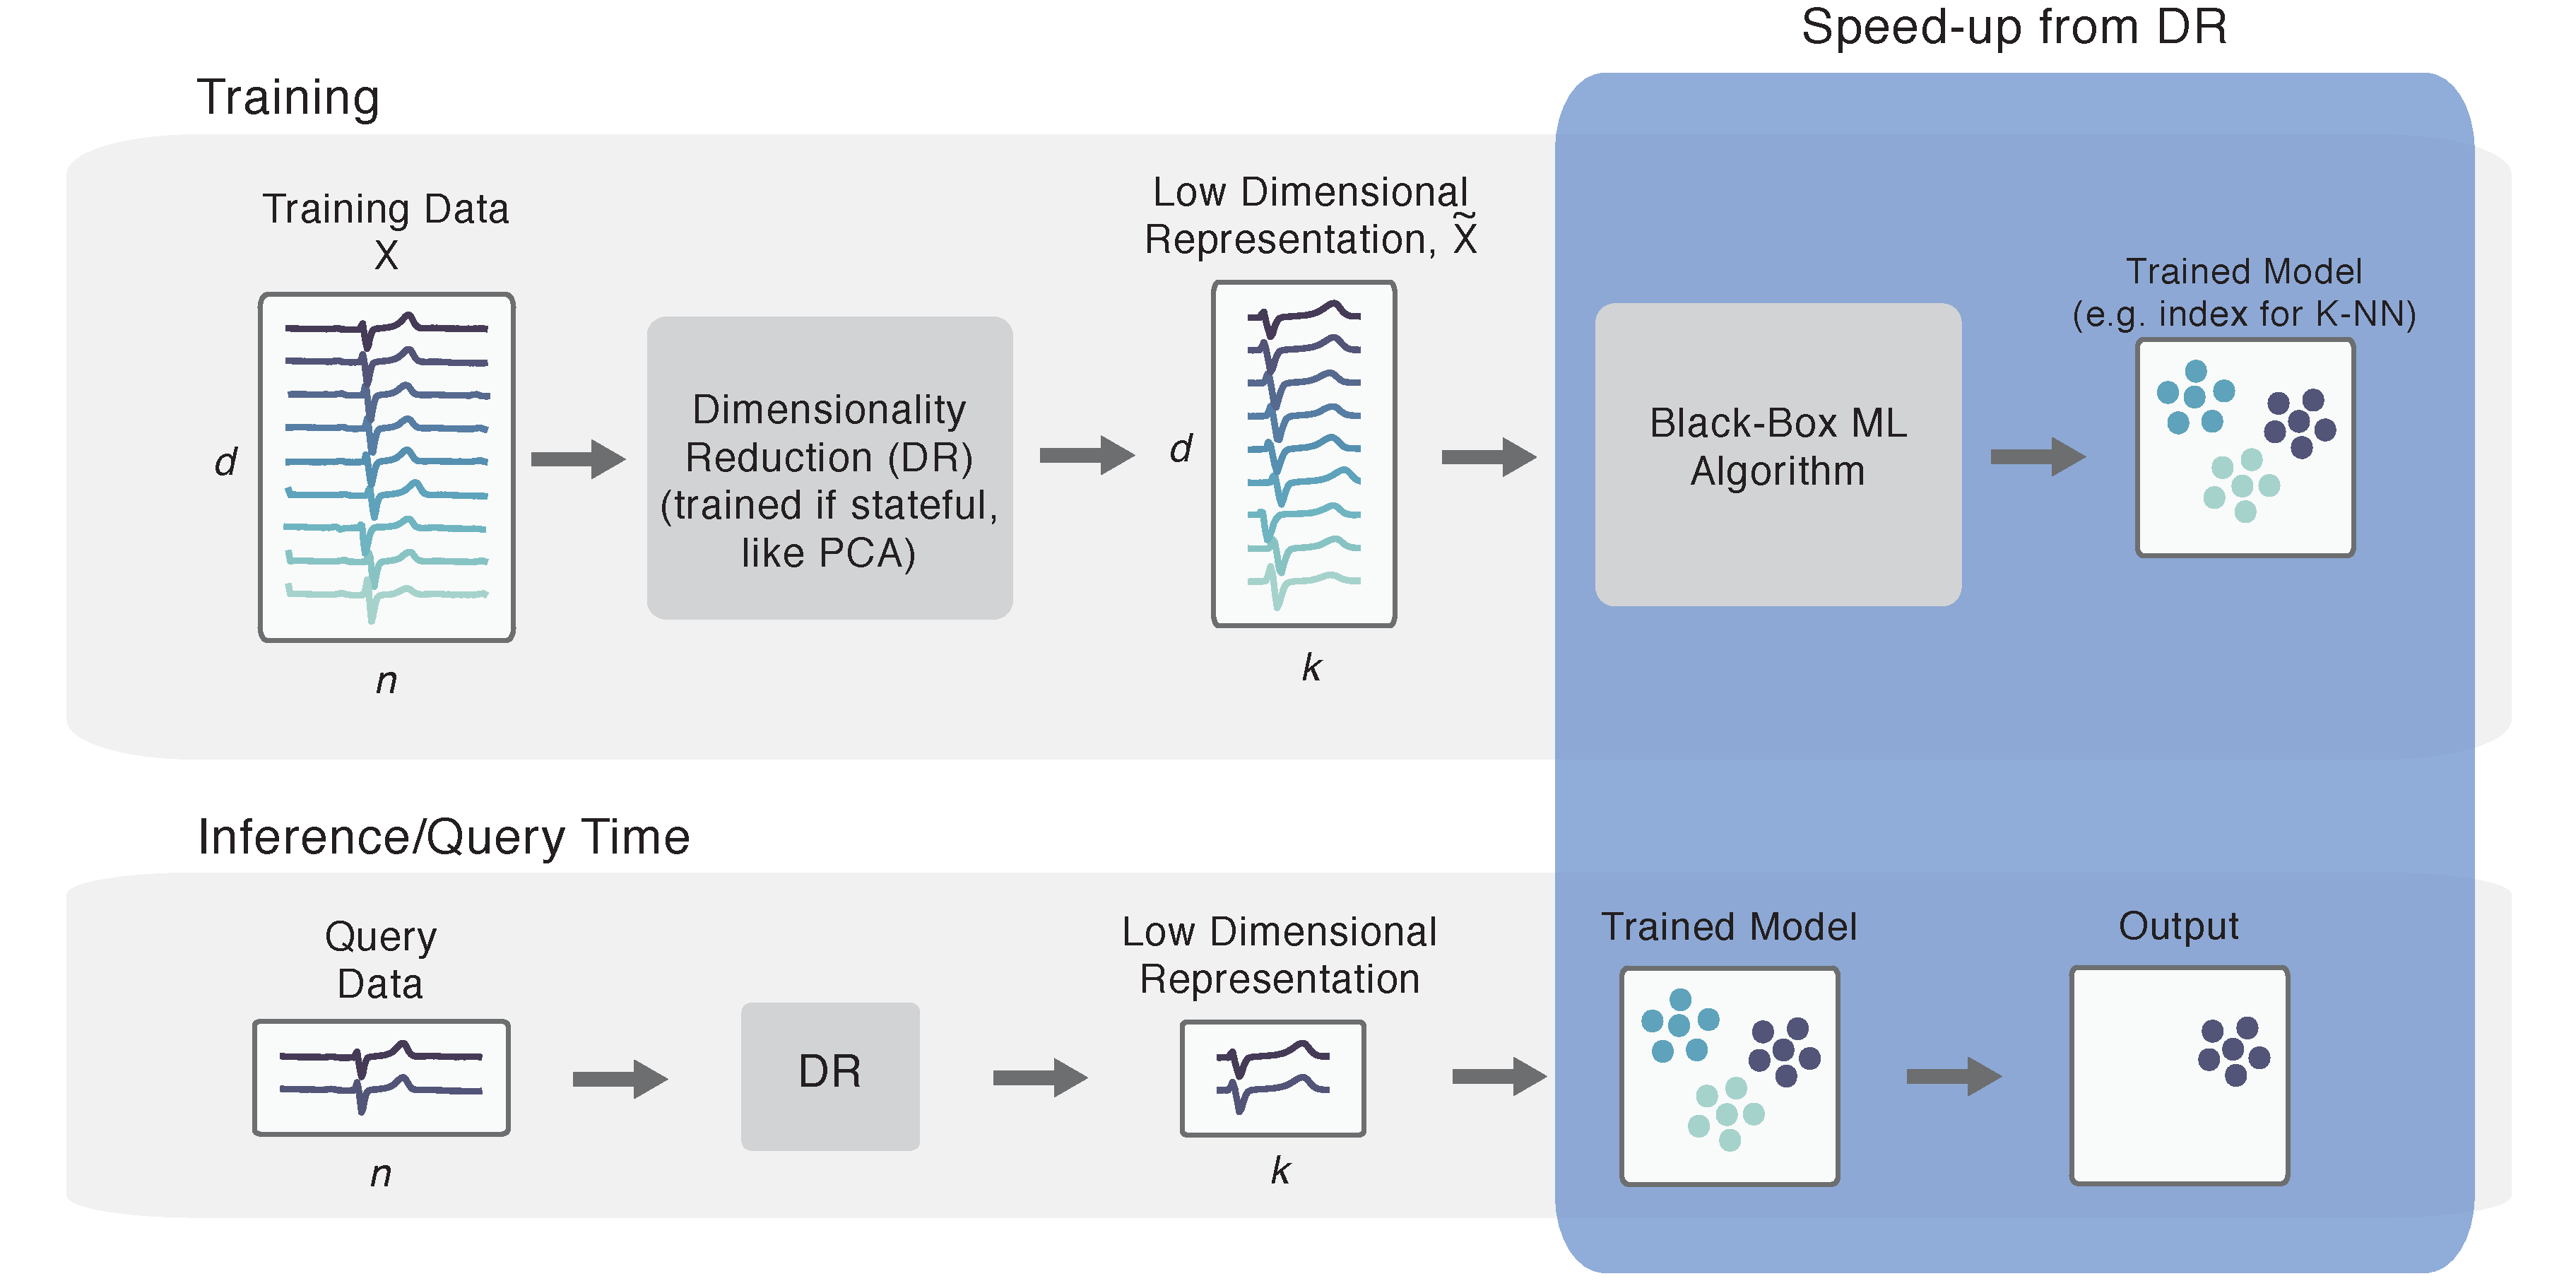
\includegraphics[width=\linewidth]{figs/pipeline.pdf}
\caption[]{Sample machine learning pipeline with dimensionality reduction. Spending time on DR provides downstream runtime speed-ups.}
\label{fig:pipeline}
\end{figure}

To this end, we develop DROP, a system that performs whole-workload runtime optimization by dynamically identifying the amount of sampling required for stochastic PCA.
DROP takes a high-dimensional dataset,\footnote{Our primary focus \red{for performance evaluation is a case study on time series similarity search,} given the amount of study in the database community~\cite{keogh-study} and the resurgence of interest in time series analytics systems~\cite{macrobase,macrobase-cidr,trill-signal}. We provide a preliminary generalizability analysis in Section~\ref{sec:experiments}.}  property to preserve (e.g., pairwise Euclidean distance to 5\%), and optional runtime model expressing downstream workload performance as a function of dimensionality (e.g., for k-Nearest Neighbors [k-NN], runtime is linear in dimensionality). 
DROP returns a low-dimensional transformation for the input using as few samples as needed to minimize the projected overall workload runtime while satisfying quality constraints.

\begin{figure}
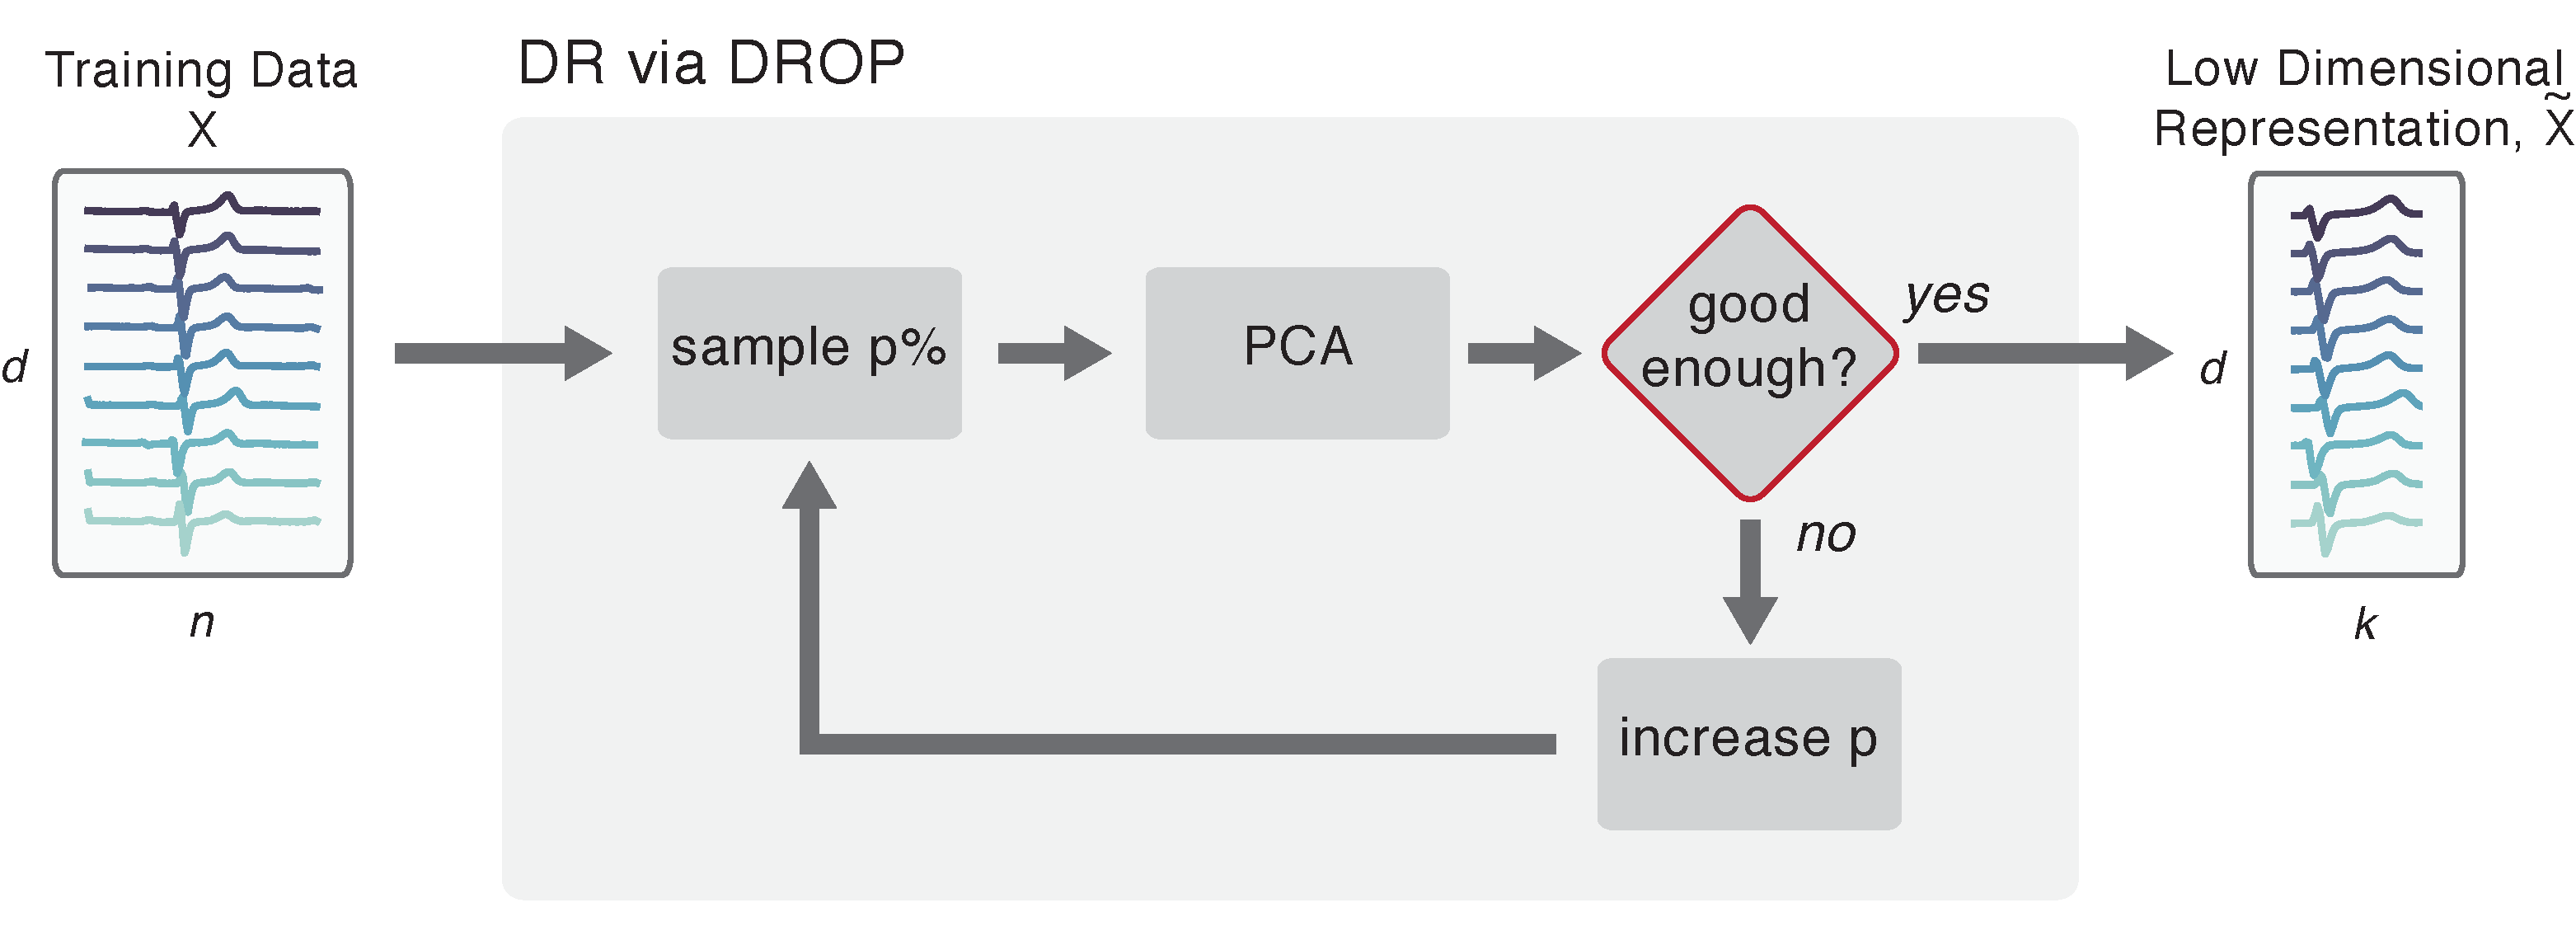
\includegraphics[width=\linewidth]{figs/basic.pdf}
\caption[]{DROP is a workload-aware DR operator compatible with standard ML pipelines. The challenge DROP solves is when to stop training (``good enough?")}
\label{fig:basic}
\end{figure}

%%%%%%

To achieve this functionality, DROP addresses the question of how much to sample the input dataset via data-dependent progressive sampling and online progress estimation at runtime.  
DROP performs PCA on a small sample to obtain a candidate transformation, then progressively increases the number of samples until termination (see Figure~\ref{fig:basic}). 
To identify the termination point that minimizes the overall runtime, DROP must overcome three challenges:

First, given the results of PCA on a data sample, DROP must \emph{evaluate the quality} of the current candidate transformation.
Popular analytics and data mining tasks often require approximate preservation of metrics such as average pairwise distances between data points~\cite{time-series-dm,dm-book}, which are costly to compute.
Thus, DROP adapts confidence intervals for fast estimation of the input metric to preserve.


Second, DROP must \emph{estimate the marginal benefit of sampling additional datapoints} for another iteration.
When running PCA on a series of progressively larger samples, later samples will incur higher computational cost but may return lower-dimensional transformations. 
To navigate this trade-off between end-to-end runtime and transformation quality, DROP uses the results obtained from previous iterations to build a predictive performance model for future iterations.


Finally, given the current quality and expected marginal benefit of the next iteration, DROP must \emph{optimize end-to-end runtime}.
While an application-agnostic approach would iterate until successive iterations yield no benefit to quality, many analytics operators such as k-Nearest Neighbors are tolerant of error~\cite{gemini}, so it is frequently advantageous to trade a slightly higher-dimensional basis for faster pre-processing (DR).
To address this challenge, the system performs workload-specific optimization to minimize the expected runtime of the complete end-to-end analytics pipeline.


\begin{comment}

PCA is guaranteed to find the optimal linear transformation with respect to $\mathcal{L}_2$ reconstruction error, popular analytics and data mining tasks (e.g., k-NN~\cite{time-series-dm}, k-means~\cite{dm-book},  kernel density estimation~\cite{wand}) instead require approximate preservation of metrics such as average pairwise distances between data points.
To overcome this challenge, DROP adapts confidence intervals (either via closed-form or, if unavailable, via bootstrapping) for fast estimation of the input metric to preserve.


Since PCA is guaranteed to find the optimal linear transformation with respect to $\mathcal{L}_2$ reconstruction error, we could consider estimating the transformation quality using this quantity.
However, many popular analytics and data mining tasks (e.g., k-NN~\cite{time-series-dm}, k-Means~\cite{dm-book},  Kernel Density Estimation~\cite{wand}) do not use reconstruction error, and instead require approximate preservation of metrics such as average pairwise distances between data points.
A transformation that minimizes reconstruction error is not guaranteed to preserve the pairwise distance by the same amount.
Moreover, na\"ively computing pairwise distances as required for k-NN is prohibitively expensive, with quadratic runtime.
To overcome this challenge, the system adapts an approach pioneered for deterministic queries in the context of online aggregation: treat quality metrics as aggregation functions and use confidence intervals (either via closed-form or, if unavailable, via bootstrapping) for fast estimation.
This approach allows DROP to accurately estimate representation quality while avoiding the overhead of exact computation.

Second, DROP must \emph{estimate the marginal benefit of continuing to sample} for another iteration.
When running PCA on a series of progressively larger samples, later samples will incur higher computational cost but may in turn return lower-dimensional transformations. 
To navigate this trade-off between end-to-end runtime and transformation quality, the system performs online progress estimation, using the results obtained from previous iterations to build a predictive performance model for future iterations.
%This allows DROP to quantify the expected benefit of continued sampling.

Finally, given the current quality and expected marginal benefit of the next iteration, DROP must \emph{optimize end-to-end runtime} to determine whether to terminate.  
The system must evaluate if the expected marginal benefit to dimensionality arising from continuing to iterate would reduce total runtime.
While an application-agnostic approach would iterate until successive iterations yield no benefit to quality, many analytics operators such as k-Nearest Neighbors are tolerant of error~\cite{gemini}, so it is frequently advantageous to trade a slightly higher-dimensional basis for faster pre-processing (DR).
To address this challenge, the system performs workload-specific optimization to minimize the expected runtime of the complete end-to-end analytics pipeline.
\end{comment}

\begin{comment}
A simple, application-agnostic approach to addressing this problem would iterate until until successive iterations yield no benefit to quality, thus converging to the lowest-dimensional metric-preserving transformation.
However, as we have hinted, many time-series analytics operators such as k-Nearest Neighbors are tolerant of approximation error~\cite{gemini}, and it is frequently advantageous to trade a slightly higher-dimensional basis for faster pre-processing. In these settings, running to convergence is often wasteful.
To address this challenge, DROP performs a workload-specific optimization, utilizing a provided (or profiled) application-specific runtime model and performs online optimization  to minimize the expected runtime of the complete end-to-end analytics pipeline.
\end{comment} 

We view DROP as a pragmatic combination of recent theoretical advances in dimensionality reduction and classic techniques from approximate query processing, and a useful system for performing end-to-end workflow optimization.
We make the following contributions in this work:
\begin{itemize}

\item We show the data sample required to perform accuracy-achieving PCA is often small (as little as $1\%$), and data-dependent sampling can enable \red{$91\times$} speedup compared to PCA via singular value decomposition (SVD). 
%We show that as little as $2\%$ of time series data suffices to preserve pairwise distances within $2\%$, providing a $55.6\times$ reduction in dimension.
  %this came from the oracle numbers--used 0.002 and then looked at table
  
\item We propose DROP, an online optimizer for DR that uses information about downstream analytics tasks to perform efficient stochastic PCA.
%. DROP uses information about downstream analytics tasks to utilize as few samples as required to minimize the overall workload runtime, while satisfying constraints on the reduction quality.

\item We present techniques based on progressive sampling, approximate query processing, online progress estimation, and cost based optimization to enable up to \red{$5\times$} faster end-to-end execution over PCA via SVD.% and up to $3\times$ faster end-to-end execution than alternative techniques on real analytics pipelines.
\end{itemize}




\section{Related Work}
\label{sec:relwork}
\label{sec:relatedwork}

\minihead{Dimensionality Reduction} DR is a
classic operation~\cite{dr-survey1,dr-survey2,trefethen,nonlinear-dr} that is
well studied in the
database~\cite{keogh-indexing,local-dr,charu-ss,dynamic-ss}, data
mining~\cite{sax,paa}, statistics and machine
learning~\cite{alecton,shamir}, and theoretical CS~\cite{bernstein,pca-stoc} communities.

Recent breakthroughs in the theoretical statistics community provided new algorithms for PCA that promise substantial scalability improvements without compromising result quality~\cite{alecton,tropp,re-new, tropp}. 
%Foremost among these techniques are advanced stochastic methods~\cite{re-new,shamir}, and techniques for randomized SVD~\cite{tropp}.
%While we default to the latter for use by DROP's PCA operator, DROP's modular architecture makes it simple to use any method in its place, including recent systems advances in scalable PCA~\cite{ppca-sigmod}.
%As a proof of concept of our method, we provide implementations of full SVD-based PCA, power iteration, as well as Oja's method. 
To the best of our knowledge, advanced methods for PCA
have not been empirically compared head-to-head with conventional
DR approaches such as Piecewise Approximate
Averaging~\cite{paa}.%, especially on real datasets. 
In addition, DROP
\emph{combines} these methods with row-level sampling to provide benefits similar to using stochastic methods for PCA.

%This setting differs from that of Moving Window (or Rolling) PCA in that the these methods assume overlap among the data samples, whereas here our samples are independently drawn from the same underlying data distribution~\cite{mwpca}.

%\red{
%\minihead{Time Series Indexing}
%While DROP is intended as a general purpose DR operator for downstream workloads, there exists a vast body of literature specific to time series indexing for similarity search. 
%While these techniques, such as iSAX2+ (and related methods)~\cite{sax,isax,isaxorig,hotsax}, SSH~\cite{ssh}, and Coconut~\cite{coconut} are highly optimized for the bulk-load and repeated query use case, DROP provides a more flexible, downstream-operator aware method. 
%}

\minihead{Approximate Query Processing} 
Inspired by approximate query processing engines~\cite{barzan-keynote}
as in online aggregation~\cite{onlineagg}, DROP performs progressive
sampling.  In contrast
with more general data dimensionality estimation
methods~\cite{dr-estimation}, DROP optimizes for
$TLB$. As we illustrated in \S\ref{sec:experiments}, this
strategy confers substantial runtime improvements.
While DROP performs simple uniform sampling, the literature contains a wealth of techniques for various biased sampling techniques~\cite{surajit-sample, surajit-2}.
Finally, DROP performs online progress estimation to minimize the
end-to-end analytics cost function. This is analogous to query
progress estimation~\cite{qpi1} and performance
prediction~\cite{mr-predict} in database and data
warehouse settings and has been exploited in approximate query
processing engines such as BlinkDB~\cite{blinkdb}. 

\minihead{Scalable \red{ Workload-Aware, }Complex Analytics} DROP is an operator
for analytics dataflow pipelines. Thus, DROP is
as an extension of recent results on integrating complex
analytics function including model training~\cite{bismarck,mcdb,mlbase} and
data exploration~\cite{scorpion,canopy,kraska-viz} operators into analytics engines. 
%\red{In particular, DROP is especially related to recent work in integrating workload-aware cost models to complex subscription forecasting models~\cite{forecasting} so as to reduce subscriber notification overhead.}

\section{Problem Statement and Background}
\label{sec:background}

In this section, we  provide background on dimensionality reduction (DR), and then define our problem of workload-aware dimensionality reduction (DR). Finally, we revisit a widely cited empirical comparison of DR techniques from VLDB 2008~\cite{keogh-study} \red{that we use as a case study to validate} that Principal Component Analysis (PCA) can outperform classic techniques, but at a high computational cost.

\subsection{Dimensionality Reduction}
\label{sec:defs}

DR refers to finding a low-dimensional representation of a dataset that preserves properties of interest, such as data point similarity~\cite{dr-survey1,dr-survey2}. Formally, consider a data matrix $X \in \mathbb{R}^{\mvar \times \dvar}$, where each row $i$ corresponds to data point $x_i \in \mathbb{R}^\dvar$, with $\mvar > \dvar$.  
DR computes a transformation function ($T: \mathbb{R}^\dvar \rightarrow \mathbb{R}^k$) that maps each $x_i$ to a new basis as $\tilde{x}_i \in \mathbb{R}^k$ where $k \leq \dvar$, resulting in a new data matrix $T(X) = \tilde{X} \in \mathbb{R}^{\mvar \times k}$.

\subsubsection*{Principal Component Analysis (PCA)}
\label{sec:pca}
PCA is a linear DR technique that identifies a new orthogonal basis for a dataset that captures its directions of highest variance.
Of all linear transformations, this basis minimizes reconstruction error in a mean square sense. 
Classically implemented PCA uses a Singular Value Decomposition (SVD) routine~\cite{trefethen}.

\begin{comment} 
\begin{algorithm}
\begin{algorithmic}[1]
\Statex \textbf{Inputs:}  
\Statex $X \in \mathbb{R}^{m_1 \times d}$: training data matrix 
\Statex $Y \in \mathbb{R}^{m_2 \times d}$: data matrix to transform 
\Statex $k \in \mathbb{Z}_+$: desired dimensionality of transformed data
\Statex \textsc{SVD-T}: any truncated SVD algorithm  
\Statex
\Statex \hrule
\Function{fit}{$X$}:
	\State $\bar{X} = \text{columnMeans}(X)$
	\State $C_X = X - \bar{X}$
		\Comment{$C_X \in \mathbb{R}^{m_1 \times d}$}
	\State \textbf{Store: } $\bar{X}, C_A$
\EndFunction

\Function{transform}{$Y, k, $ \textsc{SVD-T}}:
	\State $U, \Sigma, V^T$ = \textsc{SVD-T}$(C_X, k)$
		\Comment{$V \in \mathbb{R}^{d \times k}$}
	\State $C_Y = Y - \bar{X}$
		\Comment{$C_Y \in \mathbb{R}^{m_2 \times d}$} 
	\State \textbf{Store: } $T = V$ 
			\Comment{Cache for repeated use} \\
	\Return $C_YT$
		%\Comment{$C_BV \in \mathbb{R}^{M_2 \times k}$} 
\EndFunction

\end{algorithmic}
\caption{PCA via truncated SVD}
\label{alg:PCA-inc}
\end{algorithm}

%discuss advanced techniques
As described in Section~\ref{related}, several theoretical advances provide accelerated means of of efficiently computing PCA over large-scale data beyond the na\"ive SVD-based approach.
These methods operate on samples of input data, and---in theory---confer substantial runtime benefits when in fact a low-dimensional basis exists (i.e., the spectrum of eigenvalues has a large drop).
However, there are two main challenges in utilizing these approaches.
First, it is unclear when to stop sampling data points when using stochastic or mini-batch methods, including state-of-the-art momentum techniques that achieve accelerated convergence rates~\cite{CDS}.
This is because convergence of these techniques (e.g., the magnitude of the gradient in stochastic gradient methods) does not correspond directly to preservation of metrics of interest.
Second, these techniques typically rely the target reduced dimension ($k$) to be specified a priori, but the suitable $k$ for the task at hand is rarely known a priori for a given dataset. The choice of $k$ can dramatically affect runtimes and convergence rates, making the target dimensionality an important, yet difficult to obtain parameter. 

Thus, even with advanced techniques, it is unclear \emph{how much computation is required} to obtain acceptable low dimensional representations, and \emph{how low a dimension is considered acceptable} for specific application constraints. 
We describe how DROP overcomes these challenges in [forward ref sampling], and show how answering these questions enables improvements over previous techniques when evaluated in an end-to-end context.  
\end{comment}

\subsection{DR \red{for Repeated-Query Workloads}}

In workloads such as similarity search, clustering, \red{or classification}, ML models are periodically trained over historical data, and are \emph{repeatedly queried} as incoming data arrives or new query needs arise (see Fig~\ref{fig:pipeline}). 
Indexes built over this data can improve the efficiency of this repeated query workload in exchange for a preprocessing overhead.
DR with a multidimensional index structure is a classic way of achieving this, and is the basis for popular similarity search procedures and extensions in the data mining and machine learning communities~\cite{keogh-indexing,local-dr,charu-ss,dynamic-ss,dm-book,humming-index,decade,search}; a metric-preserving transformation reduces input dimensionality, and an index is built in this new space for subsequent queries.


\subsubsection*{\red{DR in Similarity Search}}
\red{Similarity search is a common repeated-query workload performed over a variety of data types including images, documents and time series~\cite{keogh-study,lsh}, which we use as a running case study given its popularity and the large amount of research in the space.
The Tightness of Lower Bounds ($TLB$) is typically the metric preserved by DR in this setting~\cite{keogh-study}, as it measures how well a \emph{contractive} DR transformation (i.e. distances in the transformed space are less than or equal to those in the original) preserves pairwise Euclidean distances. This can be used to identify the quality of a low dimensional transformation without performing the downstream similarity search task:}
\begin{equation}
\label{eq:tlb}
TLB = \frac{2}{\mvar(\mvar-1)}\sum_{i<j}\frac{\| \tilde{x}_i -  \tilde{x}_j \|_2 }{\| x_i -  x_j\|_2 }.
\end{equation}


\subsection{Problem: Workload-Aware DR}
\label{subsec:wadr}

In end-to-end analytics tasks, we wish to minimize the combined runtime of DR and downstream applications. 
DR is a fixed cost (i.e., in index construction for similarity search), while each query (i.e., nearest neighbor query) over the dataset incurs a marginal cost that is dependent on DR quality: lower-dimensional data points result in faster queries. 

In workload-aware dimensionality reduction, we perform DR to minimize overall workload runtime. As input, we consider a set of data points, a desired level of metric preservation ($B$; default $TLB$, e.g., $TLB \geq .99$) and, optional downstream runtime as a function of dimensionality ($\mathcal{C}_\mvar(\dvar)$ for an $\mvar\times \dvar$ data matrix).  
We use this information to efficiently return a DR function that satisfies the metric constraint with a configurable degree of confidence.
More formally, denoting DR runtime as $R$, we define the optimization problem:
\begin{problem}
\label{def:opt}
  Given $X \in \mathbb{R}^{\mvar \times \dvar}$, $TLB$ constraint $B \in 
  (0, 1]$, confidence $c$, and workload runtime function $\mathcal{C}_\mvar:\mathbb{Z}_{+} \rightarrow \mathbb{R}_{+}$, find $k$ and transformation
  matrix $T_k \in \mathbb{R}^{\dvar \times k}$ that minimizes $R + \mathcal{C}_\mvar(k)$
  such that $TLB(XT_k) \geq B$ with confidence $c$.
\end{problem}

We assume the downstream runtime model $\mathcal{C}_\mvar(\dvar)$ is monotonically increasing in $\dvar$ as the premise of DR for efficient analytics relies on downstream tasks running faster on lower dimensional data.
Absent this, we default to execution until convergence (i.e, until $k$ plateaus) as described in Section~\ref{sec:sampling}, and demonstrate the cost of doing so in Section~\ref{sec:experiments}.

The more time spent on DR ($R$), the smaller the transformation ($k$), thus the lower the workload runtime.
To minimize $R + \mathcal{C}_\mvar(k)$, we must determine how much time to spend on DR to minimize end-to-end runtime.


\subsection{Case Study: PCA Speed vs. Quality}

While improved quality provides faster repeated query execution (as seen in Section~\ref{sec:experiments}), the cost of DR via PCA dominates this speedup, encouraging the use of faster, lower-quality alternatives~\cite{keogh-study}. 
This motivates our study of downstream-workload-aware, stochastic, sampling-based PCA methods.

To briefly quantify this trade-off, we augment a widely-cited time series similarity search DR study from VLDB 2008~\cite{keogh-study} by evaluating PCA---which the authors did not benchmark due to it being ``untenable for large data sets" despite providing ``optimal linear dimensionality reduction."
We compare PCA via SVD to baseline techniques based on both runtime and DR performance with respect to $TLB$ over the largest datasets from~\cite{keogh-study}. 
We use two of their fastest methods as our baselines since they show the remainder exhibited ``very little difference'': Fast Fourier Transform (FFT) and Piecewise Aggregate Approximation (PAA).
We verify that PCA offers more effective dimensionality reduction than alternative techniques for time series similarity search, but with a large computational overhead. 


\minihead{TLB Performance Comparison}
We compute the minimum dimensionality ($k$) achieved by each technique subject to a $TLB$ constraint. 
On average across the datasets, PCA provides bases that are $2.3\times$ and $3.7\times$  smaller than PAA and FFT for $TLB = 0.75$, and $2.9\times$ and $1.8\times$ smaller for $TLB = 0.99$.
While the margin between PCA and alternatives is dataset-dependent, PCA almost always preserves $TLB$ with a lower dimensional representation.

%\section{Additional End-to-End Plots}
%\input{endendplots}

\minihead{Runtime Performance Comparison} 
PCA implemented via out-of-the-box SVD is on average over \red{$26\times$ (up to $56\times$)} slower than PAA and over \red{$4.6\times$ (up to $9.7\times$)} times slower than FFT when computing the smallest $TLB$-preserving basis.
This substantiates the observation that classic PCA is incredibly slow compared to alternatives~\cite{keogh-study}. 



%\section{Sample-Based Computation}
\label{sec:sampling}

%Stochastic PCA methods that iterate over small data samples either $i)$ execute for a pre-specified number of iterations or $ii)$ execute until convergence to the solution provided by classical PCA.
%To our knowledge, these existing termination conditions are not suitable when considering users' willingness to trade quality for downstream workload runtime.
%However, using these methods as a starting point,
We \red{augment our case study to} show that running PCA on data samples does not sacrifice DR quality, but that the number of samples required varies per dataset.
We then show how progressively increasing the sampling rate can help dynamically identify how much to sample a given dataset.

\subsection{Feasibility of Sampling}
Many real-world \red{datasets} are intrinsically low-dimensional, as evidenced by their rapid falloff in their eigenvalue spectrum.
A data sample thus captures much of the dataset's ``interesting'' behavior, so fitting a model over such a sample will generalize well. We verify this phenomenon by varying the target $TLB$ and examining the minimum number of samples required to obtain a $TLB$-preserving transform with output dimension $k$ equal to input dimension $\dvar$.

On average, across the considered UCR time series datasets, a sample of under $0.64\% (\text{up to } 5.5\%)$ of the input is sufficient for a $TLB$ of $0.75$, and under $4.15\% (\text{up to } 38.6\%)$ is sufficient for a $TLB$ of $0.99$.  
When this proportion is known a priori, we obtain up to \red{$91\times$ speedup} compared to a na\"ive implementation of PCA via SVD---with no algorithmic improvement. 


\subsection{Incremental, Progressive Sampling}
Sampling benefit is dataset-dependent; we must identify how large a sample suffices to compute high-quality transforms.
Figure~\ref{fig:progressive} shows how the dimensionality required to attain a given $TLB$ changes when we vary dataset and proportion of data sampled.
Increasing the number of samples provides lower dimensional transformations for the same quality.
However, this decrease in dimension plateaus as the number of samples increases.
Thus, we must determine when the downstream value of decreased dimension is overpowered by the cost of additional DR---that is, whether to sample to convergence (evaluated in Section~\ref{subsec:lesion}) or terminate early (e.g., at $0.3$ proportion of data sampled for SmallKitchenAppliances). 


\begin{figure}
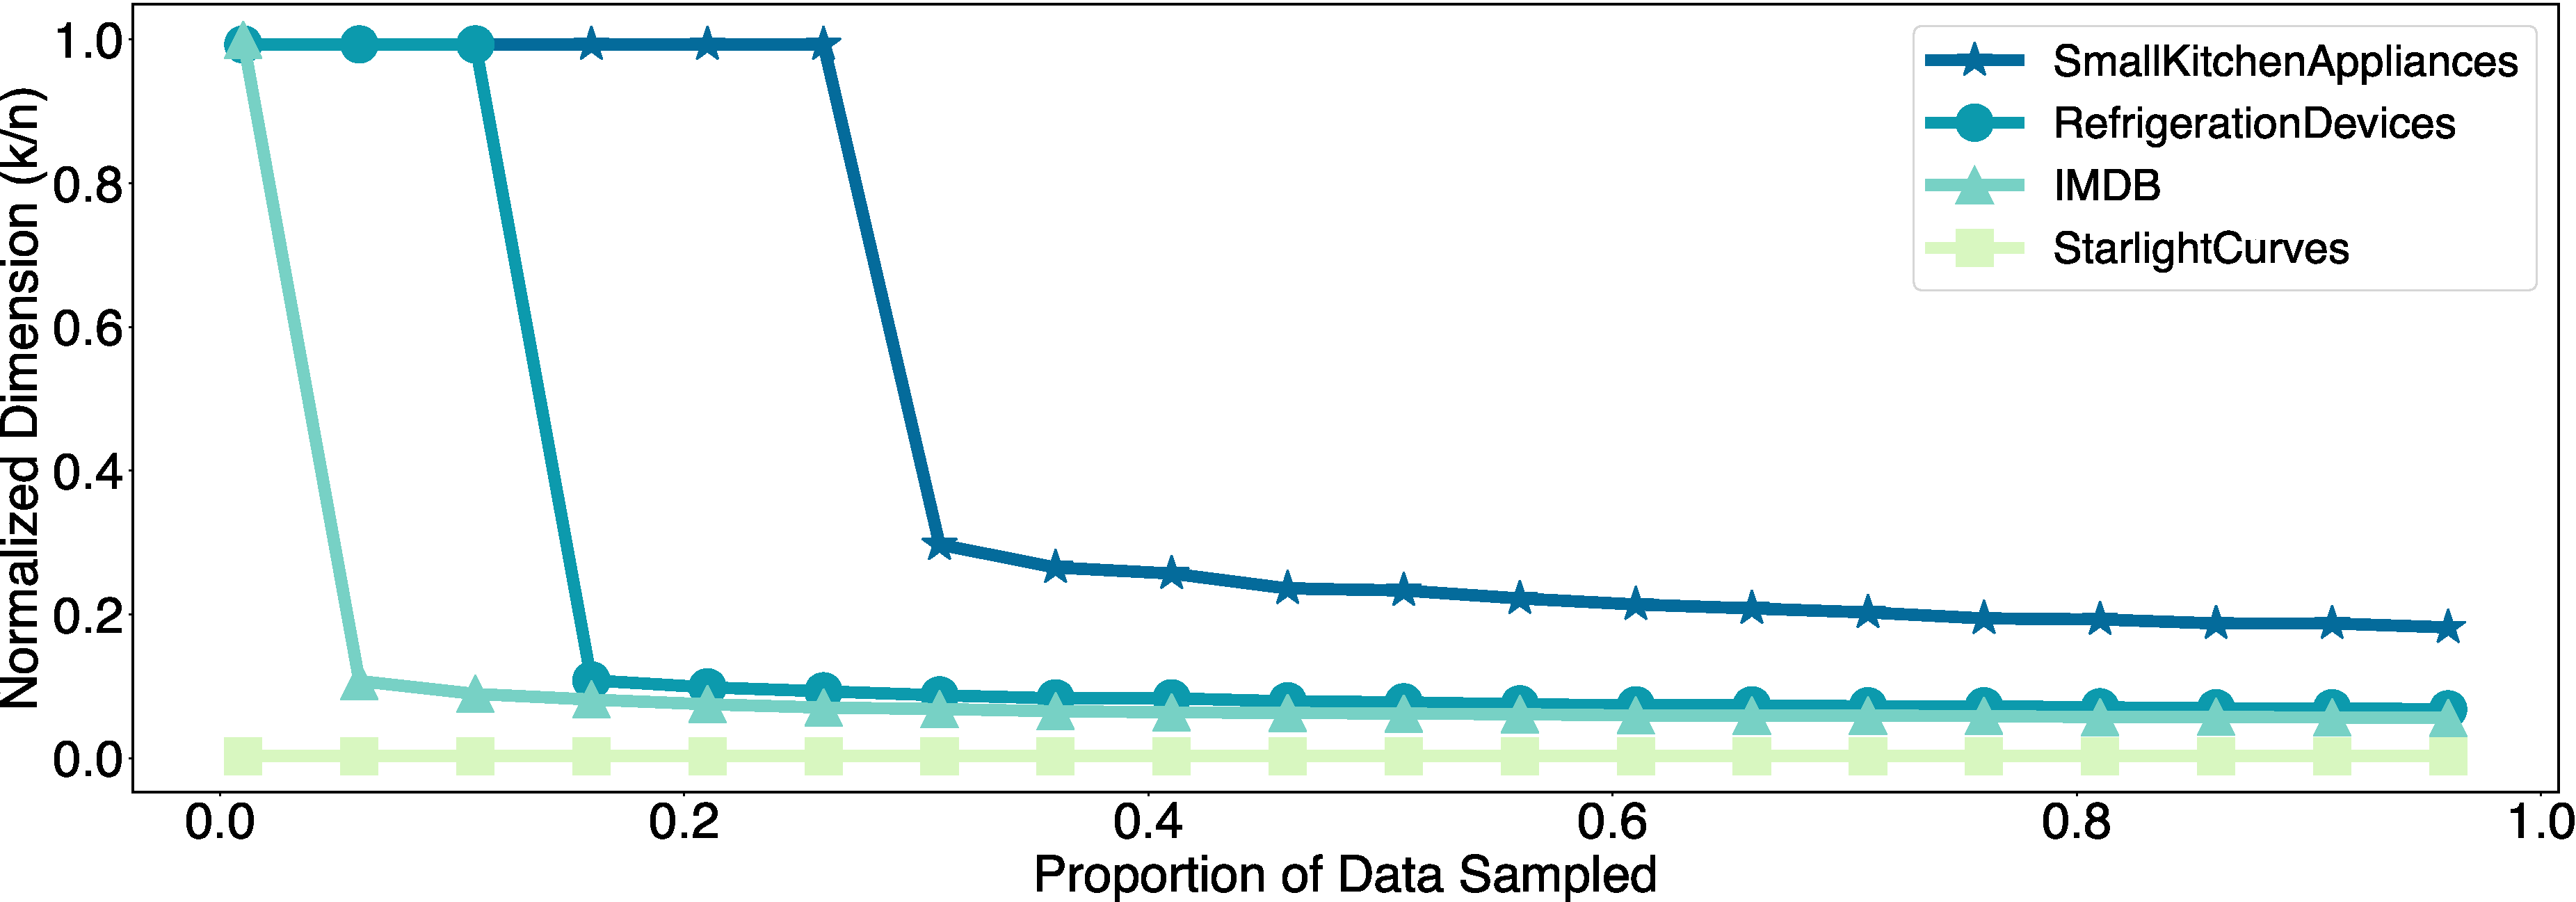
\includegraphics[width=\linewidth]{figs/progressive.pdf}
\caption[]{ Improvement in representation size for  $TLB = 0.80$ across three datasets. Higher sampling rates improve quality until reaching a state equivalent to running PCA over the full dataset ("convergence")}
\label{fig:progressive}
\end{figure}





\section{DROP: Workload Optimization}
\label{sec:algo}

In this section, we introduce DROP, a system that performs workload-aware DR via progressive sampling and online progress estimation.
DROP takes as input a target dataset, metric to preserve (default, target $TLB$), and an optional downstream runtime model.
DROP then uses sample-based PCA to identify and return a low-dimensional representation of the input that preserves the specified property while minimizing estimated workload runtime (Figure 2, Alg.~\ref{alg:DROP}).

%DROP answers a crucial question that stochastic PCA techniques have traditionally ignored: how long should these methods run? 

\begin{comment}
Notation used is in Table~\ref{table:inputs}.

\begin{table}
\centering
\small
\caption{\label{table:inputs} 
 DROP algorithm notation and defaults}
{\renewcommand{\arraystretch}{1.2}
\begin{tabular}{|c|l l|}
\hline 
Symbol & Description (\emph{Default}) & Type\tabularnewline
\hline
$X$  & Input dataset                          & $\mathbb{R}^{\mvar \times \dvar}$ \tabularnewline
$\mvar$  & Number of input data points            & $\mathbb{Z}_{+}$\tabularnewline
$\dvar$  & Input data dimension                   & $\mathbb{Z}_{+}$ \tabularnewline
$B$  & Target $TLB$ preservation      		 & $0 < \mathbb{R} \leq 1 $ \tabularnewline
$\mathcal{C}_\mvar(\dvar)$  & Downstream runtime function (\textit{k-NN runtime})       & $\mathbb{Z}_{+} \to \mathbb{R}_{+}$\tabularnewline
$R$  & Total DROP runtime       & $\mathbb{R}_{+}$ \tabularnewline
$c$ & Confidence level for $TLB$ preservation (\textit{$95 \%$})          & $\mathbb{R}$  \tabularnewline
$T_k$  & DROP output $k$-dimensional transformation &$\mathbb{R}^{\dvar \times k}$ \tabularnewline
$i $ & Current DROP iteration        & $\mathbb{Z}_+$  \tabularnewline

\hline 
\end{tabular}
}
\end{table}
\end{comment}

\begin{figure}
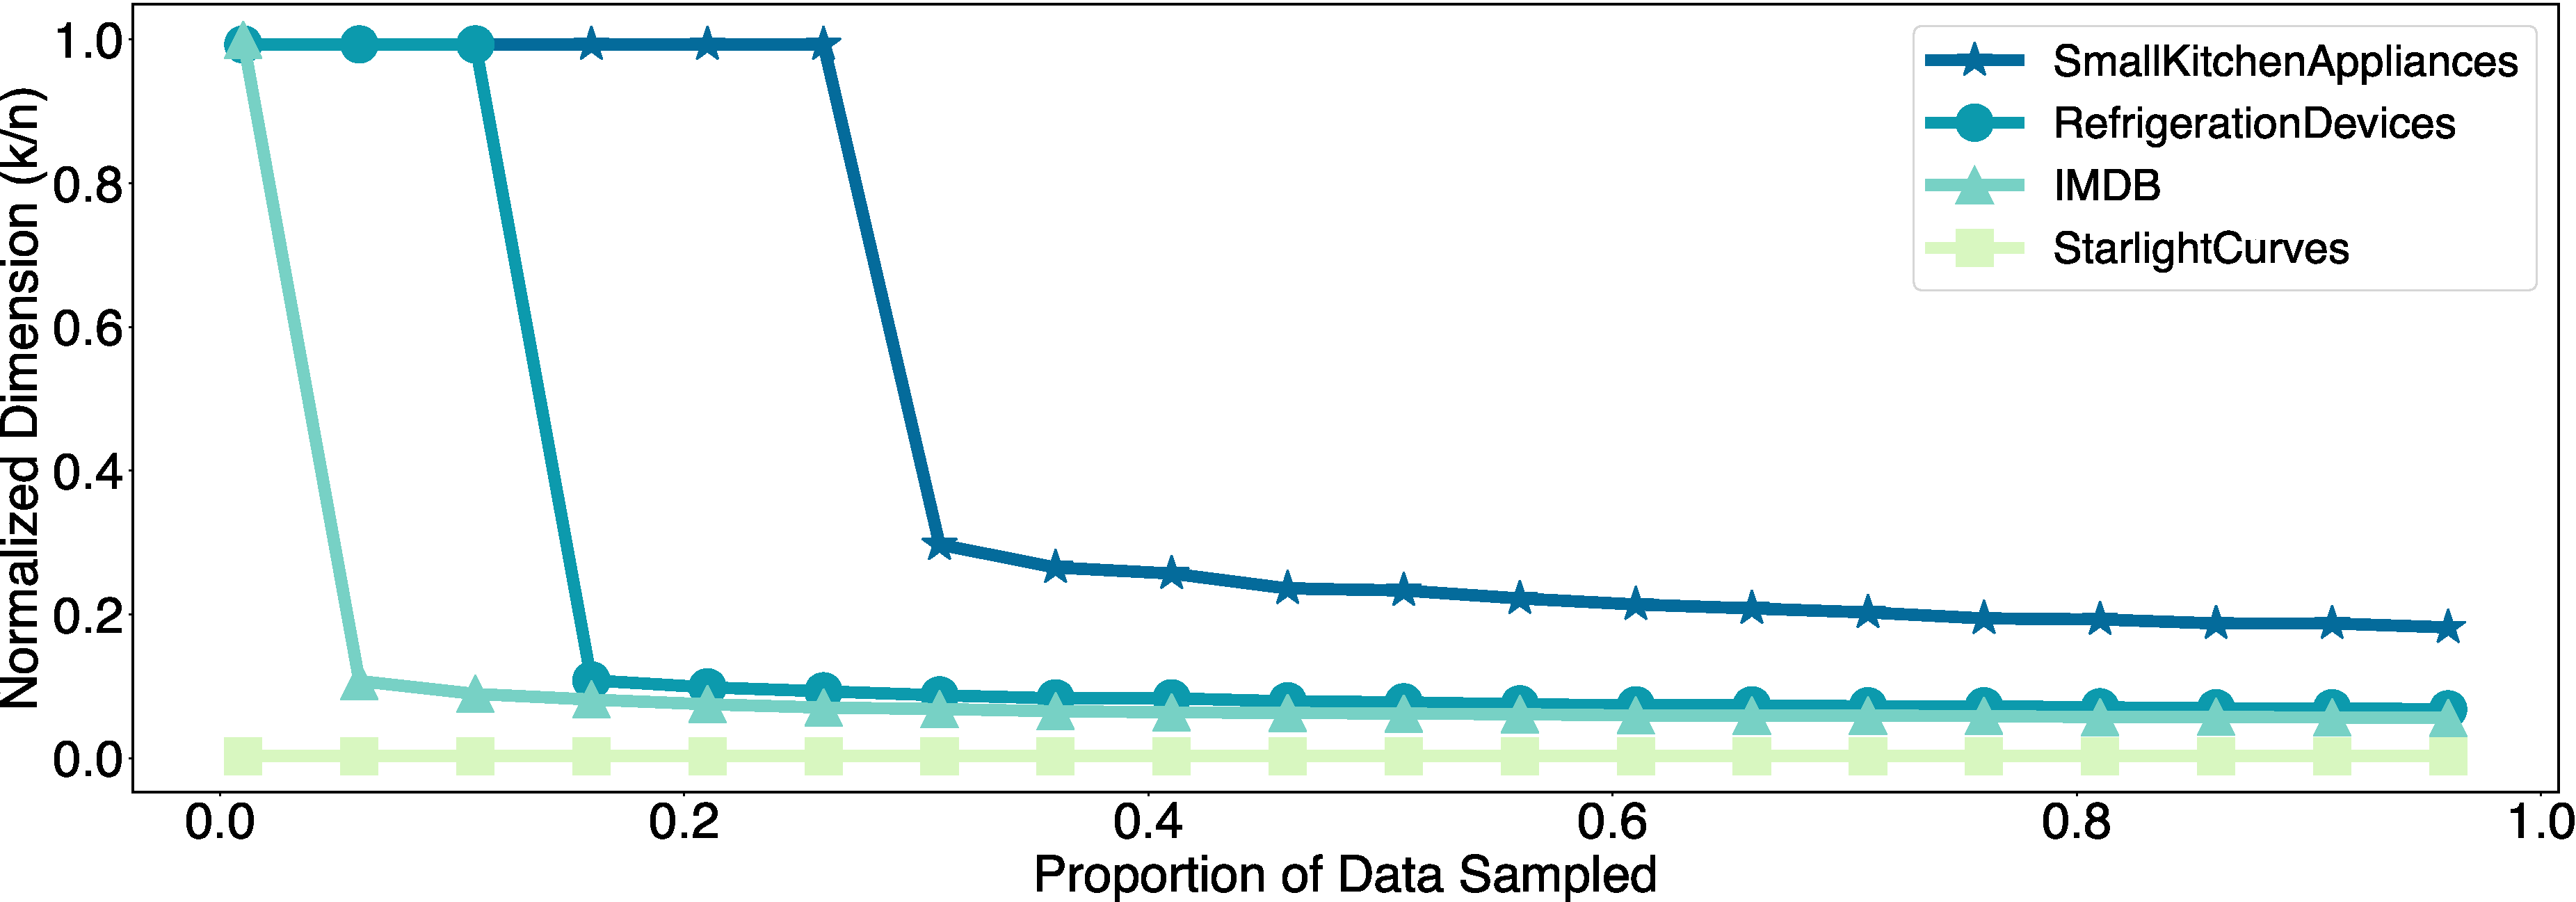
\includegraphics[width=\linewidth]{figs/progressive.pdf}
\caption[]{ Reduction in dimensionality for  $TLB = 0.80$ with progressive sampling. Dimensionality decreases until reaching a state equivalent to running PCA over the full dataset ("convergence").}
\label{fig:progressive}
\end{figure}

\subsection{DROP Algorithm}
\label{subsec:arch}
%DROP is a system that performs workload-aware dimensionality reduction, optimizing the combined runtime of downstream tasks and DR as defined in Problem~\ref{def:opt}.
DROP operates over a series of data samples, and determines when to terminate via \red{a} four-step procedure at each iteration: %progressive sampling, transformation evaluation, progress estimation, and cost-based optimization:

%To power this pipeline, DROP combines database and machine learning techniques spanning online aggregation (\S\ref{subsec:teval}), progress estimation (\S\ref{subsec:pest}), progressive sampling (\S\ref{subsec:psample}), and PCA approximation (\S\S\ref{subsec:pcaroutine},\ref{subsec:reuse}).

%We now provide a brief overview of DROP's sample-based iterative architecture before detailing each.

\begin{comment}
\item Progressive Sampling (\S\ref{subsec:psample}): DROP draws a data sample, performs PCA over it, and uses of a novel reuse mechanism across iterations (\S\ref{subsec:reuse}).

\item Transform Evaluation (\S\ref{subsec:teval}): DROP evaluates the above by identifying the size of the smallest metric-preserving transformation that can be extracted. 

\item Progress Estimation (\S\ref{subsec:pest}): Given the size of the smallest metric-preserving transform and the time required to obtain this transform, DROP estimates the size and computation time of continued iteration.

\item Cost-Based Optimization (\S\ref{subsec:opt}): DROP optimizes over DR and downstream task runtime to determine if it should terminate.
\end{comment}

\minihead{Step 1: Progressive Sampling (\S\ref{subsec:psample})}

\noindent DROP draws a data sample, performs PCA over it, and uses of a novel reuse mechanism across iterations (\S\ref{subsec:reuse}).

\minihead{Step 2: Transform Evaluation (\S\ref{subsec:teval})} 

\noindent DROP evaluates the above by identifying the size of the smallest metric-preserving transformation that can be extracted. 

\minihead{Step 3: Progress Estimation (\S\ref{subsec:pest})} 

\noindent Given the size of the smallest metric-preserving transform and the time required to obtain this transform, DROP estimates the size and computation time of continued iteration.

\minihead{Step 4: Cost-Based Optimization (\S\ref{subsec:opt})} 

\noindent DROP optimizes over DR and downstream task runtime to determine if it should terminate.

\subsection{Progressive Sampling}
\label{subsec:psample}

Inspired by stochastic PCA methods (\S\ref{sec:relatedwork}), DROP uses sampling to tackle workload-aware DR. 
Many real-world \red{datasets} are intrinsically low-dimensional; a small data sample is sufficient to characterize dataset behavior. 
To verify, we extend our case study (\S\ref{sec:RQW}) by computing how many uniformly selected data samples are required to obtain a $TLB$-preserving transform with $k$ equal to input dimension $\dvar$.
On average, a sample of under $0.64\%$ $(\text{up to } 5.5\%)$ of the input is sufficient for $TLB = 0.75$, and under $4.2\%$ $(\text{up to } 38.6\%)$ is sufficient for $TLB=0.99$.  
If this sample rate is known, we obtain up to \red{$91\times$ speedup} over PCA via SVD.%---with no algorithmic improvement. 

However, this benefit is dataset-dependent, and unknown a priori.
We thus turn to progressive sampling (gradually increasing the sample size) to identify how large a sample suffices.
Figure~\ref{fig:progressive} shows how the dimensionality required to attain a given $TLB$ changes when we vary dataset and proportion of data sampled.
Increasing the number of samples (which increases PCA runtime) provides lower $k$ for the same $TLB$.
However, this decrease in dimension plateaus as the number of samples increases.
Thus, while progressive sampling allows DROP to tune the amount of time spent on DR, DROP must determine when the downstream value of decreased dimension is overpowered by the cost of DR---that is, whether to sample to convergence or terminate early (e.g., at $0.3$ proportion of data sampled for SmallKitchenAppliances). 


Concretely, DROP first repeatedly chooses a subset of data and computes a $\dvar$-dimensional transformation via PCA on the subsample, and then proceeds to determine if continued sampling is beneficial to end-to-end runtime.
We consider a simple uniform sampling strategy: each iteration, DROP samples a fixed percentage of the data.
 
 
 
 
 
%Exploring data-dependent and weighted sampling schemes that are dependent on the current basis is an exciting area for future work. 
%While we considered a range of alternative sampling strategies, uniform sampling strikes a balance between computational and statistical efficiency. 
%Data-dependent and weighted sampling schemes that are dependent on the current basis may decrease the total number of iterations required by DROP, but may require expensive reshuffling of data at each iteration~\cite{coresets}. 

%DROP provides configurable strategies for both base number of samples and the per-iteration increment, in our experimental evaluation in \S\ref{sec:experiments}, we consider a sampling rate of $1\%$ per iteration.
%We discuss more sophisticated additions to this base sampling schedule in the extended manuscript.

\begin{algorithm}[t!]
\begin{algorithmic}[1]
\small
\Statex \textbf{Input:}  $X$: data; $B$: target metric preservation level; $\mathcal{C}_\mvar$: cost of downstream operations
\Statex \textbf{Output:} $T_k$: $k$-dimensional transformation matrix
\Statex
\Statex \hrule
\Function{drop}{$X,  B, \mathcal{C}_\mvar$}:
	\State Initialize: $i = 0; k_0 = \infty$ 
		\Comment{iteration and current basis size}
	\Do
		\State i$\texttt{++}$, \textsc{clock.restart}
		\State $X_i$ = \textsc{sample}($X, \textsc{sample-schedule}(i)$) \label{eq:sample}
			\Comment{\S~\ref{subsec:psample}}
		\State $T_{k_i}$ = \textsc{compute-transform}($X, X_i,  B$) \label{eq:evaluate}
			\Comment{\S~\ref{subsec:teval}}
		\State $r_i = \textsc{clock.elapsed}$	
			\Comment{$R = \sum_i r_i$}
		\State $\hat{k}_{i+1}, \hat{r}_{i+1} $ = \textsc{estimate}($k_i, r_i$) \label{eq:estimate}
			\Comment{\S~\ref{subsec:pest}}
	\doWhile{\textsc{optimize}($\mathcal{C}_\mvar,k_i,r_i,\hat{k}_{i+1}, \hat{r}_{i+1}$)} \label{eq:optimize}
		\Comment{\S~\ref{subsec:opt}}
	\\\Return{$T_{k_i}$}
\EndFunction
\end{algorithmic}
\caption{DROP Algorithm}
\label{alg:DROP}
\end{algorithm}



\subsection{Transform Evaluation}
\label{subsec:teval}
DROP must accurately and efficiently evaluate this iteration's performance with respect to the metric of interest \red{over the entire dataset}. 
%To do so, DROP adapts an approach for deterministic queries in online aggregation: treating quality metrics as aggregation functions and using confidence intervals for fast estimation. 
%We first discuss this approach in the context of $TLB$, then discuss how to extend this approach to alternative metrics at the end of this section.
We define this iteration's performance as the size of the lowest dimensional $TLB$-preserving transform ($k_i$) that it can return. 
There are two challenges in performance evaluation.
First, the lowest $TLB$-achieving $k_i$ is unknown a priori. 
Second, brute-force $TLB$ computation would dominate the runtime of computing PCA over a sample. 
We now describe how to solve these challenges.

\subsubsection{Computing the Lowest Dimensional Transformation}

Given the $\dvar$-dimensional transformation from step 1, to reduce dimensionality, DROP must determine if a smaller dimensional $TLB$-preserving transformation can be obtained and return the smallest such transform. 
Ideally, the smallest $k_i$ would be known a priori, but in practice, this is not true---thus, DROP uses the $TLB$ constraint and two properties of PCA to automatically identify it.
%A na\"ive strategy would evaluate the $TLB$ for every combination of the $\dvar$ basis vectors for every transformation size, requiring $O(2^\dvar)$ evaluations. 
%Instead, DROP exploits two key properties of PCA to avoid this.

First, PCA via SVD produces an orthogonal linear transformation where the principal components  are returned in order of decreasing dataset variance explained.
As a result, once DROP has computed the transformation matrix for dimension $\dvar$, DROP obtains the transformations for all dimensions $k$ less than $\dvar$ by truncating the matrix to $\dvar \times k$ .
%PCA via SVD produces an orthogonal linear transformation where the first principal component explains the most variance in the dataset, the second explains the second most---subject to being orthogonal to the first---and so on.  

Second, with respect to $TLB$ preservation, the more principal components that are retained, the better the lower-dimensional representation in terms of $TLB$.  
This is because orthogonal transformations such as PCA preserve inner products. 
Therefore, an $\dvar$-dimensional PCA perfectly preserves $\ell_2$-distance between data points. 
As $\ell_2$-distance is a sum of squared (positive) terms, the more principal components retained, the better the representation preserves $\ell_2$-distance.

Using the first property, DROP obtains all low-dimensional transformations for the sample from the $\dvar$-dimensional basis.  
Using the second property, DROP runs binary search over these transformations to return the lowest-dimensional basis that attains $B$ (Alg.~\ref{alg:candidate}, l\ref{eq:basis}).
If $B$ cannot be realized with this sample, DROP omits further optimization steps and continues the next iteration by drawing a larger sample.

Additionally, computing the full $\dvar$-dimensional basis at every iteration may be wasteful. 
Thus, if DROP has found a candidate $TLB$-preserving basis of size $\dvar' < \dvar$ in prior iterations, then DROP only computes $\dvar'$ components at the start of the next iteration.
This allows for more efficient PCA computation for future iterations, as advanced PCA routines can exploit the $\dvar'$-th eigengap to converge faster (\S\ref{sec:relatedwork}).
% \red{This is because similar to a hold-out or validation set, $TLB$ evaluation is representative of the entire dataset, not just the current sample (see Alg.~\ref{alg:candidate} L5). 
%Thus, sampling additional training datapoints enables DROP to better learn global data structure and perform at least as well as over a smaller sample.}


% stop here!

\subsubsection{Efficient $TLB$ Computation}

Given a transformation, DROP must determine if it preserves the desired $TLB$.
Computing pairwise $TLB$ for all data points requires $O(\mvar^2\dvar)$ time, which dominates the runtime of computing PCA on a sample.
However, as the $TLB$ is an average of random variables bounded from 0 to 1, DROP can use sampling and confidence intervals to compute the $TLB$ to arbitrary confidences.

Given a transformation, DROP iteratively refines an estimate of its $TLB$ (Alg.~\ref{alg:candidate}, l\ref{eq:eval}) by \red{incrementally sampling an increasing number of} pairs from the input data (Alg.~\ref{alg:candidate}, l\ref{eq:paircheck}), transforming each pair into the new basis, then measuring the distortion of $\ell_2$-distance between the pairs, providing a $TLB$ estimate to confidence level $c$ (Alg.~\ref{alg:candidate}, l\ref{eq:tlbeval}). 
If the confidence interval's lower bound is greater than the target $TLB$, the basis is a sufficiently good fit; if its upper bound is less than the target $TLB$, the basis is not a sufficiently good fit. 
If the confidence interval contains the target $TLB$,  \red{ DROP cannot determine if the target $TLB$ is achieved. 
Thus, DROP automatically samples additional pairs to refine its estimate.
%in practice, and especially for our initial target time series datasets, DROP rarely uses more than 500 pairs on average in its $TLB$ estimates (often using far fewer)
}

To estimate the $TLB$ to confidence $c$, DROP uses the Central Limit Theorem: computing the standard deviation of a set of sampled pairs' $TLB$ measures and applying a confidence interval to the sample according to the $c$.
%For low variance data, DROP evaluates a candidate basis with few samples from the dataset \red{as the confidence intervals shrink rapidly}. 

The techniques in this section are presented in the context of $TLB$, but can be applied to any downstream task and metric for which we can compute confidence intervals and are monotonic in number of principal components retained.

\begin{comment}
\red{For instance, DROP can operate while using all of its optimizations when using any $L^p$-norm.}
\red{Euclidean similarity search} is simply one such domain that is a good fit for PCA: when performing DR via PCA, as we increase the number of principal components, a clear positive correlation exists between the percent of variance explained and the $TLB$ regardless of data spectrum.
We demonstrate this correlation in the experiment below, where we generate three synthetic datasets with predefined spectrum (right), representing varying levels of structure present in real-world datasets. 
The positive correlation is evident (left) despite the fact that the two do not directly correspond ($x=y$ provided as reference). 
This holds true for all of the evaluated real world datasets.

\vspace{.2cm}
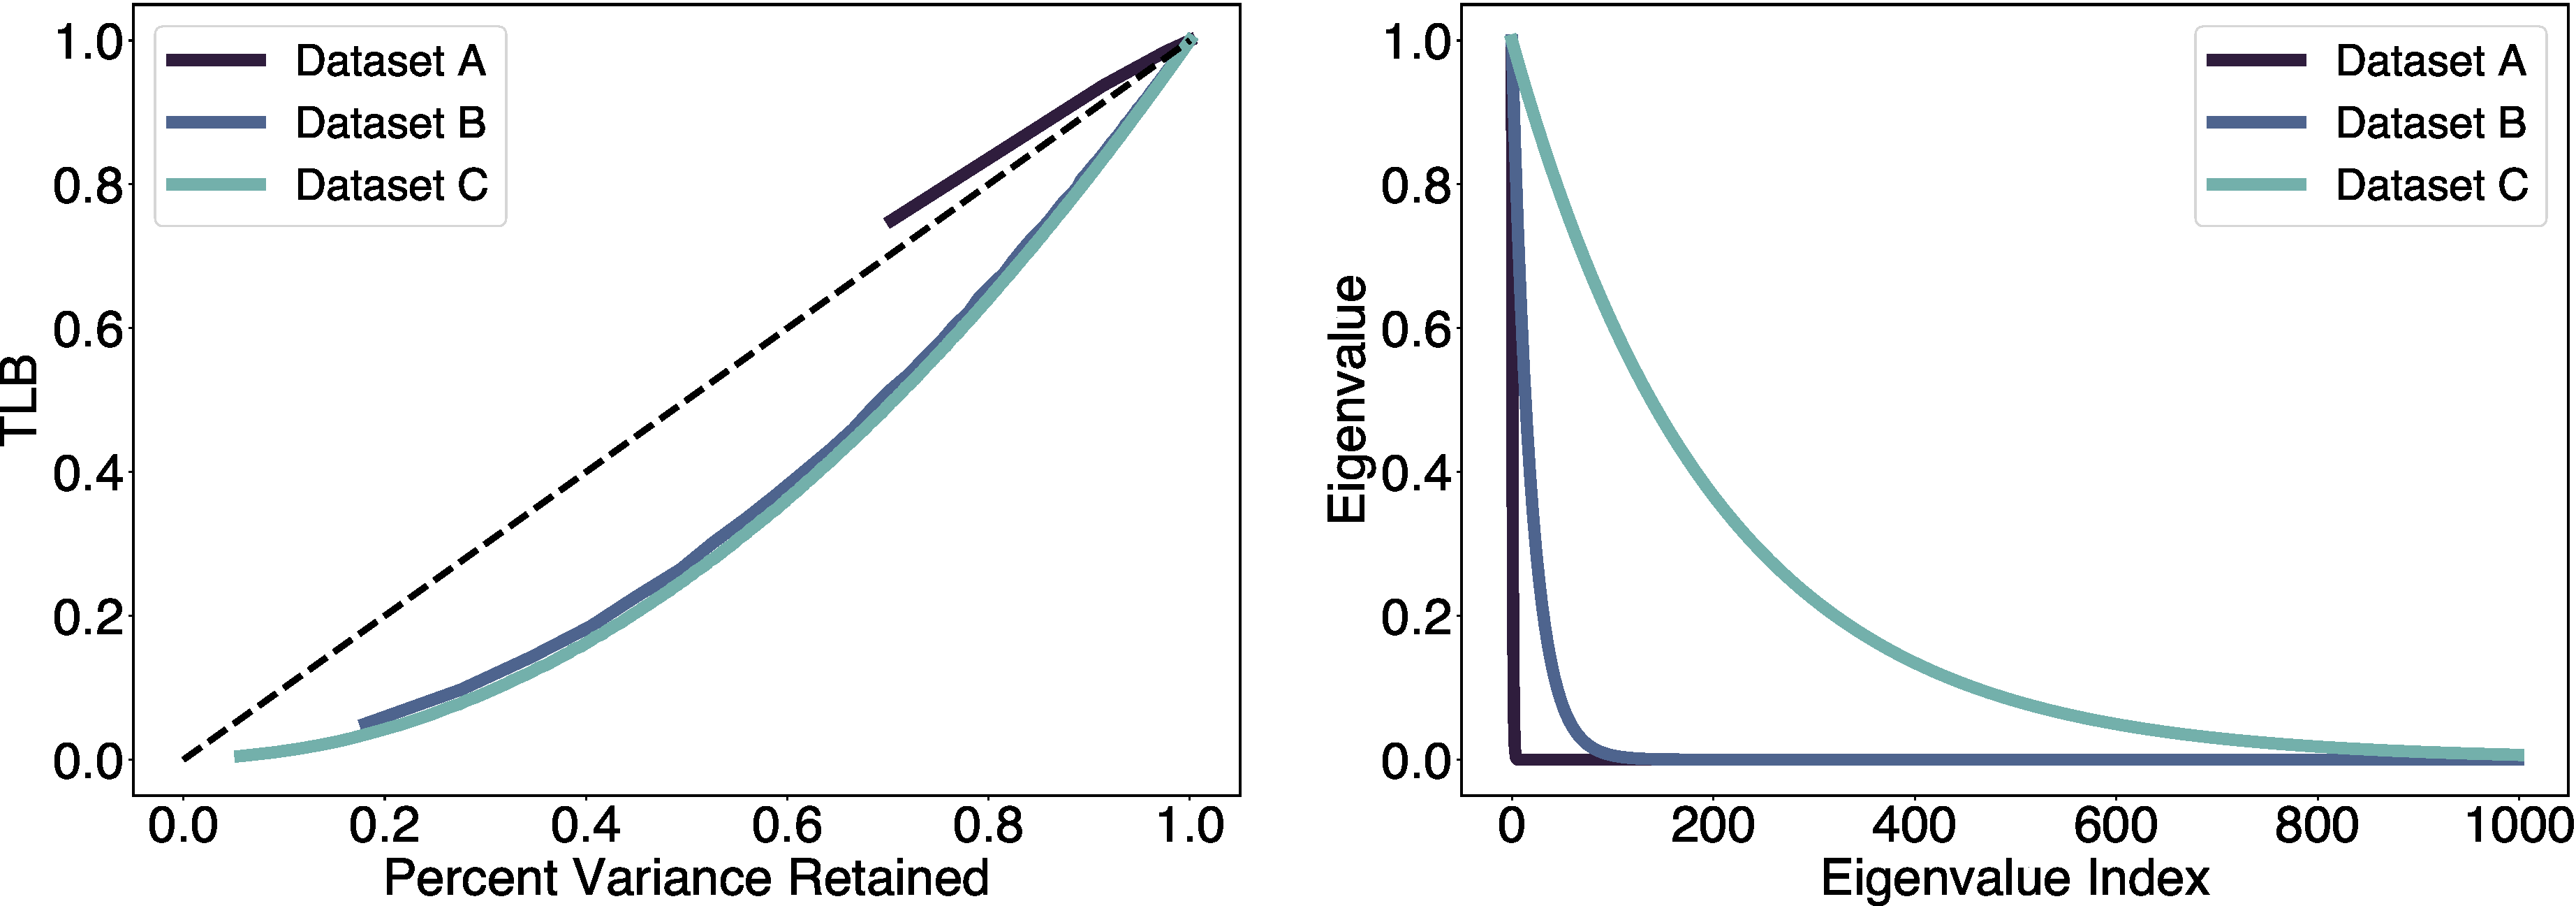
\includegraphics[width= .9\linewidth]{figs/tlb-pca.pdf}

For alternative preservation metrics, we can utilize closed-form confidence intervals~\cite{stats-book,ci1,onlineagg}, or bootstrap-based methods~\cite{bootstrap1,bootstrap2}, which incur higher overhead but can be more generally applied.
\end{comment}

\begin{algorithm}
\begin{algorithmic}[1]
\small
\Statex \textbf{Input:}  
\Statex $X$: sampled data matrix
\Statex $B$: target metric preservation level; default $TLB = 0.98$
\Statex  \hrule 
\Function{compute-transform}{$X, X_i B$}: \label{eq:basis}
	\State \textsc{pca.fit}$(X_i)$
			\Comment{fit PCA on the sample}
	\State Initialize: high $= k_{i-1}$; low $=0$; $k_i= \frac{1}{2}$(low + high); $B_i = 0$
	\While{(low $!=$ high)}
		\State $T_{k_i}, B_i  = \textsc{evaluate-tlb}( X, B, k_i)$
		\If{$B_i \leq B$}  low $= k_i + 1$ 
		\Else  \hspace{0pt} high $= k_i $
		\EndIf
		\State $k_i = \frac{1}{2}$(low + high)
	\EndWhile
	\State $T_{k_i} = $ cached $k_i$-dimensional PCA transform\\
	\Return $T_{k_i}$
\EndFunction
\Statex 
\Function{evaluate-tlb}{$X, B, k$}: \label{eq:eval}
	\State numPairs $= \frac{1}{2}\mvar(\mvar-1)$
	\State $p = 100$
		\Comment{number of pairs to check metric preservation}
	\While{($p < $ numPairs)}
		\State $B_i, B_{lo}, B_{hi} = $ \textsc{tlb}($ X, p, k$)
			 \label{eq:paircheck}
		\If{($B_{lo} > B$ or $B_{hi} < B$)}   \textbf{break}
		\Else \hspace{0pt} pairs $\times$= $ 2$
		\EndIf
	\EndWhile
	\\\Return $B_i$	
\EndFunction
\Statex 
\Function{tlb}{$X, p, k$}: \label{eq:tlbeval}
	\State \textbf{return } mean and 95\%-CI of the $TLB$ after transforming $p$ $d$-dimensional pairs of points from $X$ to dimension $k$. The highest transformation computed thus far is cached to avoid recomputation of the transformation matrix.
\EndFunction

\end{algorithmic}
\caption{Basis Evaluation and Search}
\label{alg:candidate}
\end{algorithm}


\subsection{Progress Estimation}
\label{subsec:pest}
%Given a low dimensional $TLB$-achieving transformation from the evaluation step, DROP must identify the dimensionality $k_i$ and runtime ($r_i$) of the transformation that would be obtained from an additional DROP iteration.
%We refer to this as the $progress estimation$ step.

Recall that the goal of workload-aware DR is to minimize $R + \mathcal{C}_\mvar(k)$ such that $TLB(XT_k) \geq B$, with $R$ denoting total DR (i.e., DROP's) runtime, $T_k$ the $k$-dimensional $TLB$-preserving transformation of data $X$ returned by DROP, and $\mathcal{C}_\mvar(k)$ the workload cost function. 
Therefore, given a $k_i$-dimensional transformation $T_{k_i}$ returned by the evaluation step of DROP's $i^{\text{th}}$ iteration, DROP can compute the value of this objective function by substituting its elapsed runtime for $R$ and $T_{k_i}$ for $T_k$.  
We denote the value of the objective at the end of iteration $i$ as $obj_i$. 

To decide whether to continue iterating to find a lower dimensional transform, we show in  \S\ref{subsec:opt} that DROP must estimate $obj_{i+1}$. To do so, DROP must estimate the runtime required for iteration $i+1$ (which we denote as $r_{i+1}$, where $R=\sum_i r_i$ after $i$ iterations) and the dimensionality of the $TLB$-preserving transformation produced by iteration $i+1$, $k_{i+1}$. 
DROP cannot directly measure $r_{i+1}$ or $k_{i+1}$ without performing iteration $i+1$, thus performs online progress estimation. Specifically, DROP performs online parametric fitting to compute future values based on prior values for $r_{i}$ and $k_i$ (Alg.~\ref{alg:DROP}, l\ref{eq:estimate}). 
By default, given a sample of size $m_i$ in iteration $i$, DROP performs linear extrapolation to estimate $k_{i+1}$ and $r_{i+1}$. The estimate of $r_{i+1}$, for instance, is:

\vspace{-.4cm}
\begin{equation*}
\hat{r}_{i+1} = r_i + \frac{r_i - r_{i-1}}{m_i - m_{i-1}} (m_{i+1} -  m_i).
\end{equation*}

\begin{comment}
\red{
DROP's use of a basic first-order approximation is motivated by the fact that when adding a small number of data samples each iteration, both runtime and resulting lower dimension do not change drastically (i.e., see Fig.~\ref{fig:progressive} after a feasible point is achieved). 
While linear extrapolation acts as a proof-of-concept for progress estimation, the architecture can incorporate more sophisticated functions as needed (\S\ref{sec:relwork}).
}
\end{comment}

\subsection{Cost-Based Optimization}
\label{subsec:opt}

DROP must determine if continued PCA on additional samples will improve overall runtime. 
%We refer to this as the $cost-based optimization$ step. 
Given predictions of the next iteration's runtime ($\hat{r}_{i+1}$) and dimensionality ($\hat{k}_{i+1}$), DROP uses a greedy heuristic to estimate the optimal stopping point.
If the estimated objective value is greater than its current value ($obj_i < \widehat{obj}_{i+1}$), DROP will terminate. 
If DROP's runtime is convex in the number of iterations, we can prove that this condition is the optimal stopping criterion via convexity of composition of convex functions. 
This stopping criterion leads to the following check at each iteration (Alg.\ref{alg:DROP}, l\ref{eq:optimize}): 

\vspace{-.4cm}
\begin{align}
  obj_i &< \widehat{obj}_{i+1} \nonumber \\
  \mathcal{C}_\mvar(k_i) + \sum_{j=0}^i r_j &< \mathcal{C}_\mvar(\hat{k}_{i+1}) + \sum_{j=0}^{i} r_j + \hat{r}_{i+1} \nonumber \\
  % \mathcal{C}_\mvar(k_i)  &< \mathcal{C}_\mvar(\hat{k}_{i+1}) + \hat{r}_{i+1}  \nonumber \\
  \mathcal{C}_\mvar(k_i) - \mathcal{C}_\mvar(\hat{k}_{i+1}) &< \hat{r}_{i+1}  \label{eq:check}
\end{align}

DROP terminates when the projected time of the next iteration exceeds the estimated downstream runtime benefit. 
%Absent $\mathcal{C}_d$, we default to execution until convergence (i.e, $k$ plateaus), and show the cost of doing so in \S\ref{sec:experiments}.


\begin{comment}
\red{In the general case as the rate of decrease in dimension ($k_i$) is data dependent, thus convexity is not guaranteed. 
Should $k_i$ plateau before continued decrease, DROP will terminate prematurely. 
This occurs during DROP's first iterations if sufficient data to meet the $TLB$ threshold at a dimension lower than $\dvar$ has not been sampled (SmallKitchenAppliances in Fig.~\ref{fig:progressive}).
Thus, optimization is only enabled once a feasible point is attained, as we prioritize accuracy over runtime (i.e., $0.3$ for SmallKitchenAppliances).
We show the implications of this decision in DROP in \S\ref{subsec:arch}.%, and in the streaming setting in the extended manuscript.
}
\end{comment}

\subsection{Choice of PCA Subroutine}
\label{subsec:pcaroutine}

The most straightforward means of implementing PCA via SVD in DROP is computationally inefficient compared to DR alternatives (\S\ref{sec:background}).  
DROP computes PCA via a randomized SVD algorithm from~\cite{tropp} (SVD-Halko).
Alternative efficient methods for PCA exist (i.e., PPCA, which we also provide), but we found that SVD-Halko is asymptotically of the same running time as techniques used in practice, is straightforward to implement, is $2.5-28\times$ faster than our baseline implementations of SVD-based PCA, PPCA, and Oja's method, and does not require hyperparameter tuning for batch size, learning rate, or convergence criteria.  
%While SVD-Halko is not as efficient as other techniques with respect to communication complexity as in~\cite{ppca-sigmod}, or convergence rate as in~\cite{re-new}, these techniques can be easily substituted for SVD-Halko in DROP's architecture.
%%%%We demonstrate this by implementing multiple alternatives in \S\ref{subsec:pcaexp}.
%%%%\red{Further, we also demonstrate that this implementation is competitive with the widely used SciPy Python library~\cite{scipy}}.

\begin{comment}
\begin{algorithm}[t]
\begin{algorithmic}
\State \textbf{Input:}  \\
$H$: concatenation of previous transformation matrices \\
$T$: new sample's transformation \\
 points to sample per iteration; default 5\% \\
 
\\ \hrule

\Function{distill}{$H, T$}:
	\State $H \gets [H | T]$
		\Comment{Horizontal concatenation to update history}
	\State $U, \Sigma, V^\intercal \gets \textsc{SVD}(H)$ 
				\Comment{$U$ is a basis for the range of $T$}
	\State $T \gets U[:,\textsc{num-columns(T)}]$
	\\\Return{$T$}
\EndFunction
\end{algorithmic}
\caption{Work Reuse}
\label{alg:reuse}
\end{algorithm} 
\end{comment}

\subsection{Work Reuse}
\label{subsec:reuse}

A natural question arises due to DROP's iterative architecture: can we combine information across each sample's transformations without computing PCA over the union of the data samples? 
Stochastic PCA methods enable work reuse across samples as they iteratively refine a single transformation matrix, but other methods do not.
%We propose an algorithm that allows reuse of previous work when utilizing arbitrary PCA routines with DROP.
DROP uses two insights to enable work reuse over any PCA routine.

First, given PCA transformation matrices $T_1$ and $T_2$, their horizontal concatenation $H = [T_1 | T_2]$ is a transformation into the union of their range spaces.
Second, principal components returned from running PCA on repeated data samples generally concentrate to the true top principal components for datasets with rapid spectrum drop off.
Work reuse thus proceeds as follows:
DROP maintains a transformation history consisting of the horizontal concatenation of all transformations to this point, computes the SVD of this matrix, and returns the first $k$ columns as the transformation matrix. 

Although this requires an SVD computation, computational overhead is dependent on the size of the history matrix, not the dataset size.
This size is proportional to the original dimensionality $\dvar$ and size of lower dimensional transformations, which are in turn proportional to the data's intrinsic dimensionality and the $TLB$ constraint.
As preserving \emph{all history} can be expensive in practice, 
DROP periodically shrinks the history matrix using DR via PCA. 
We validate the benefit of using work reuse---up to \red{15\%} on real-world data---in \S\ref{sec:experiments}.



\section{Experimental Evaluation}
\label{sec:experiments}

We evaluate DROP's efficiency along three dimensions: runtime, accuracy, and extensibility. We demonstrate that (1) DROP outperforms PAA and FFT in end-to-end, repetitive-query workloads, (2) DROP's optimizations each contribute to performance,  and (3) DROP extends beyond time series.

\begin{comment}
\begin{enumerate}[itemsep=0.5em]
\item{DROP outperforms PAA and FFT in end-to-end, repetitive-query workloads (\S\ref{subsec:runtime}).}	
\item{DROP's optimizations for sampling, downstream task and work reuse contribute to performance (\S\ref{subsec:lesion}).}
\item{DROP's DR runtime scales with intrinsic dimensionality, independently of data size (\S\ref{subsec:scale}).}
\item{DROP extends beyond our time series case study (\S\ref{subsec:nonts}).}	
\end{enumerate}
\end{comment}

\subsection{Experimental Setup}
\label{subsec:setup}
\minihead{Implementation} We implement DROP as an in-memory, batch-oriented feature transformation dataflow operator in Java using \red{the multi-threaded Matrix-Toolkits-Java (MTJ) library~\cite{mtj} and netlib-java~\cite{netlib} linked against Intel MKL~\cite{mkl} for compute-intensive linear algebra operations. 
We use multi-threaded JTransforms~\cite{jtransforms} for FFT, and implement multi-threaded PAA from scratch.}
%To provide an apples-to-apples comparison with our single-core PAA implementation, we disable multithreading in MTJ---enabling multi-core will equally improve all PCA-based methods across the board, including DROP, relative to PAA.
We use \red{the} Statistical Machine Intelligence and Learning Engine (SMILE) library~\cite{smile} for k-NN with different index structures\red{, and k-means}. 

\begin{comment}
\minihead{Environment} We use a server with \red{two Intel Xeon E5-2690v4 @ 2.60Ghz CPUs, each with 14 physical and 28 virtual cores (with hyper-threading). The server contains 512GB of RAM.}
We exclude data loading and parsing time.
\end{comment}

\minihead{Datasets} 
%To showcase DROP's performance in an end-to-end setting and contributions from each optimization, we use several real world datasets.
We first consider the UCR Time Series Classification Archive~\cite{ucr} for indexing experiments and lesion studies. 
We exclude datasets with fewer than 1 million entries, and fewer datapoints than dimensionality, leaving 14 datasets. 
%We also consider a larger, labeled earthquake dataset from XXX~\cite{quake}.

Due to the relatively small size of these time series datasets, we consider three additional datasets to showcase tangible wall-clock runtime improvements with DROP.
We use the standard MNIST hand-written digits dataset~\cite{mnist}, the FMA featurized music dataset~\cite{fma}, and a labeled sentiment analysis IMBD dataset~\cite{imdb}, which also demonstrates extensibility beyond time series data. 

\minihead{DROP Configuration} We use a runtime cost function for k-NN obtained via linear interpolation on data of varying dimension (implemented via cover trees~\cite{ctree}, K-D trees~\cite{kdtree},or brute force search in SMILE).
To evaluate the sensitivity to cost model, we also report on the effect of operating without a cost model (i.e., sample until convergence) in Section~\ref{subsec:lesion}.
We set $TLB$ constraints such that the accuracy of K-NN tasks remain unchanged before and after indexing via DR, corresponding to $B = 0.99$  for the UCR datasets.
Unless otherwise specified, we use a default sampling schedule that begins with and increases by $1\%$ of the input.
It is possible to optimize (and possibly overfit) this schedule for our target time series, but we provide a conservative, more general schedule.
%%%%We further discuss sampling schedules and properties that make a dataset amenable to DROP in Section~\ref{subsec:disc}. 

\minihead{Baselines} We report runtime, accuracy, and reduced dimension compared to FFT, PAA, PCA via SVD-Halko, and PCA via SVD. 
Each computes a transformation over the entire data, then performs binary search to identify the smallest dimensional basis that satisfies the target $TLB$. 
%%%%We further discuss choice of PCA subroutine in Section~\ref{subsec:pcaexp}. 

\minihead{Similarity Search/k-NN Setup} 
While many methods for similarity search exist, as in~\cite{keogh-study}, we consider k-NN in our evaluation as it is classically used and  interoperates with new use cases including one-shot learning and deep metric learning~\cite{knn1, knn2, knn3}.
%\red{Further, adopting k-NN (and, k-means in Section~\ref{subsec:nonts}), which is not a classically supported relational operator, as our target task demonstrates that simple runtime estimation routines can be extended to time-series-specific  operators.}
To evaluate DR performance when used with downstream indexes, we vary k-NN's multidimensional index structure: cover trees, K-D trees, or no index. 

End-to-end performance depends on the number of queries in the workload, and DROP is optimized for the repeated-query use case. 
Due to the small size of the UCR datasets, we choose a 1:50 ratio of data indexed to number of query points, and vary this index-query ratio in later microbenchmarks and experiments. 
We also provide a cost model for assessing the break-even point that balances the cost of a given DR technique against it's indexing benefits to each query point.


\begin{figure*}[t!]
\includegraphics[width=\linewidth]{figs/KNNraw-revision.pdf}
\caption[]{End-to-End DR and k-NN runtime (top three) and returned lower dimension (bottom) over the largest UCR datasets for three different indexing routines. DROP consistently returns lower dimensional bases than conventional alternatives (FFT, PAA), and is on average faster than PAA and FFT.}
\label{fig:knnAll}
\end{figure*}


\subsection{DROP Performance}
\label{subsec:runtime}


We evaluate DROP's performance compared to PAA and FFT using the time series case study. 

\minihead{k-NN Performance} We summarize DROP's results on an end-to-end 1-Nearest Neighbor classification in Figure~\ref{fig:knnAll}.
We display the end-to-end runtime of DROP, PAA, and FFT for each of the considered index structures: no index, K-D trees, cover trees. 
We display the size of the returned dimension for the no indexing scenario, as the other two scenarios return near \red{identical values.
This occurs as many of the datasets used in this experiment are small and possess low intrinsic dimensionality; DROP's cost model thus determines to quickly identify this dimensionality prior to termination. 
}
We do not display k-NN accuracy as all techniques meet the $TLB$ constraint, and achieve the same accuracy within $1\%$.

On average, DROP returns transformations that are $2.3\times$ and  $1.4\times$ smaller than PAA and FFT, translating to significantly smaller k-NN query time. 
End-to-end runtime with DROP is on average \red{$2.2\times$ and $1.4\times$ (up to $10\times$ and $3.9\times$)} faster than PAA and FFT, respectively, when using brute force linear search,  \red{$2.3\times$ and $1.2\times$ (up to $16\times$ and $3.6\times$)}  faster when using K-D trees, and \red{$1.9\times$ and $1.2\times$ (up to $5.8\times$ and $2.6\times$)} faster when using cover trees.
When evaluating Figure~\ref{fig:knnAll}, it becomes clear that DROP's runtime improvement is data dependent for both smaller datasets, and for datasets that do not possess a low intrinsic dimension (such as Phoneme, elaborated on in Section~\ref{subsec:lesion})
Determining if DROP is a good fit for a dataset is an exciting area for future work (\S\ref{subsec:disc}).

%We demonstrate in our lesion study in Section~\ref{subsec:lesion} that DROP also outperforms our baseline PCA via SVD implementation, as well as our SVD-Halko implementation. 

%When evaluating Figure~\ref{fig:knnAll}, it becomes clear that DROP's runtime improvement is data dependent for both smaller datasets, and for datasets that do not possess a low intrinsic dimension (such as Phoneme, elaborated on in Section~\ref{subsec:lesion}). 
%Thus, in the end of the evaluation section, we provide guidelines on how to determine if DROP is a good fit for a dataset. 

\minihead{Varying Index-Query Ratio}

DROP is optimized for highly structured data and a low index-query ratio, as in many streaming and/or high-volume data use cases.
If there are many more data points queried than used for training/constructing an index, DROP will outperform alternatives. 
A natural question that arises is in which scenarios is it beneficial to use DROP, and in which would a lower quality but faster reduction suffice. 
Domain experts are typically aware of the scale of their query workloads. 
However, we also provide a heuristic to answer this question given rough runtime and cardinality estimates of the downstream task at hand and the choice of alternative DR technique.

Let $x_d$ and $x_a$ be the per-query runtime of running a downstream task with the output of DROP and a given alternative method, respectively. 
Let $r_d$ and $r_a$ denote the amortized per-datapoint runtime of DROP and the alternative method, respectively. 
Let $n_i$ and $n_q$ the number of indexed and queried points. 
DROP is faster when $n_q x_d + n_i r_d < n_q x_a + n_i r_a$.

To verify, we obtained estimates of the above and compared DROP against FFT and PAA in lower-query-volume scenarios when running k-NN using cover trees, and display the results in Figure~\ref{fig:query}.
We first found that in the 1:1 index-query ratio setting, DROP should be slower than PAA and FFT, as observed. 
However, as we decrease the ratio, DROP becomes faster, with a break-even point of slightly lower than 1:3. 
We show that DROP does indeed outperform PAA \red{and FFT} in the 1:5 index-query ratio case, where it is is on average \red{$1.51\times$} faster than PAA and \red{$1.03\times$} faster than FFT. 
As the ratio decreases to 1:50, DROP is \red{$1.24\times$} faster than FFT and \red{$1.9\times$} faster than PAA.  


\begin{figure}
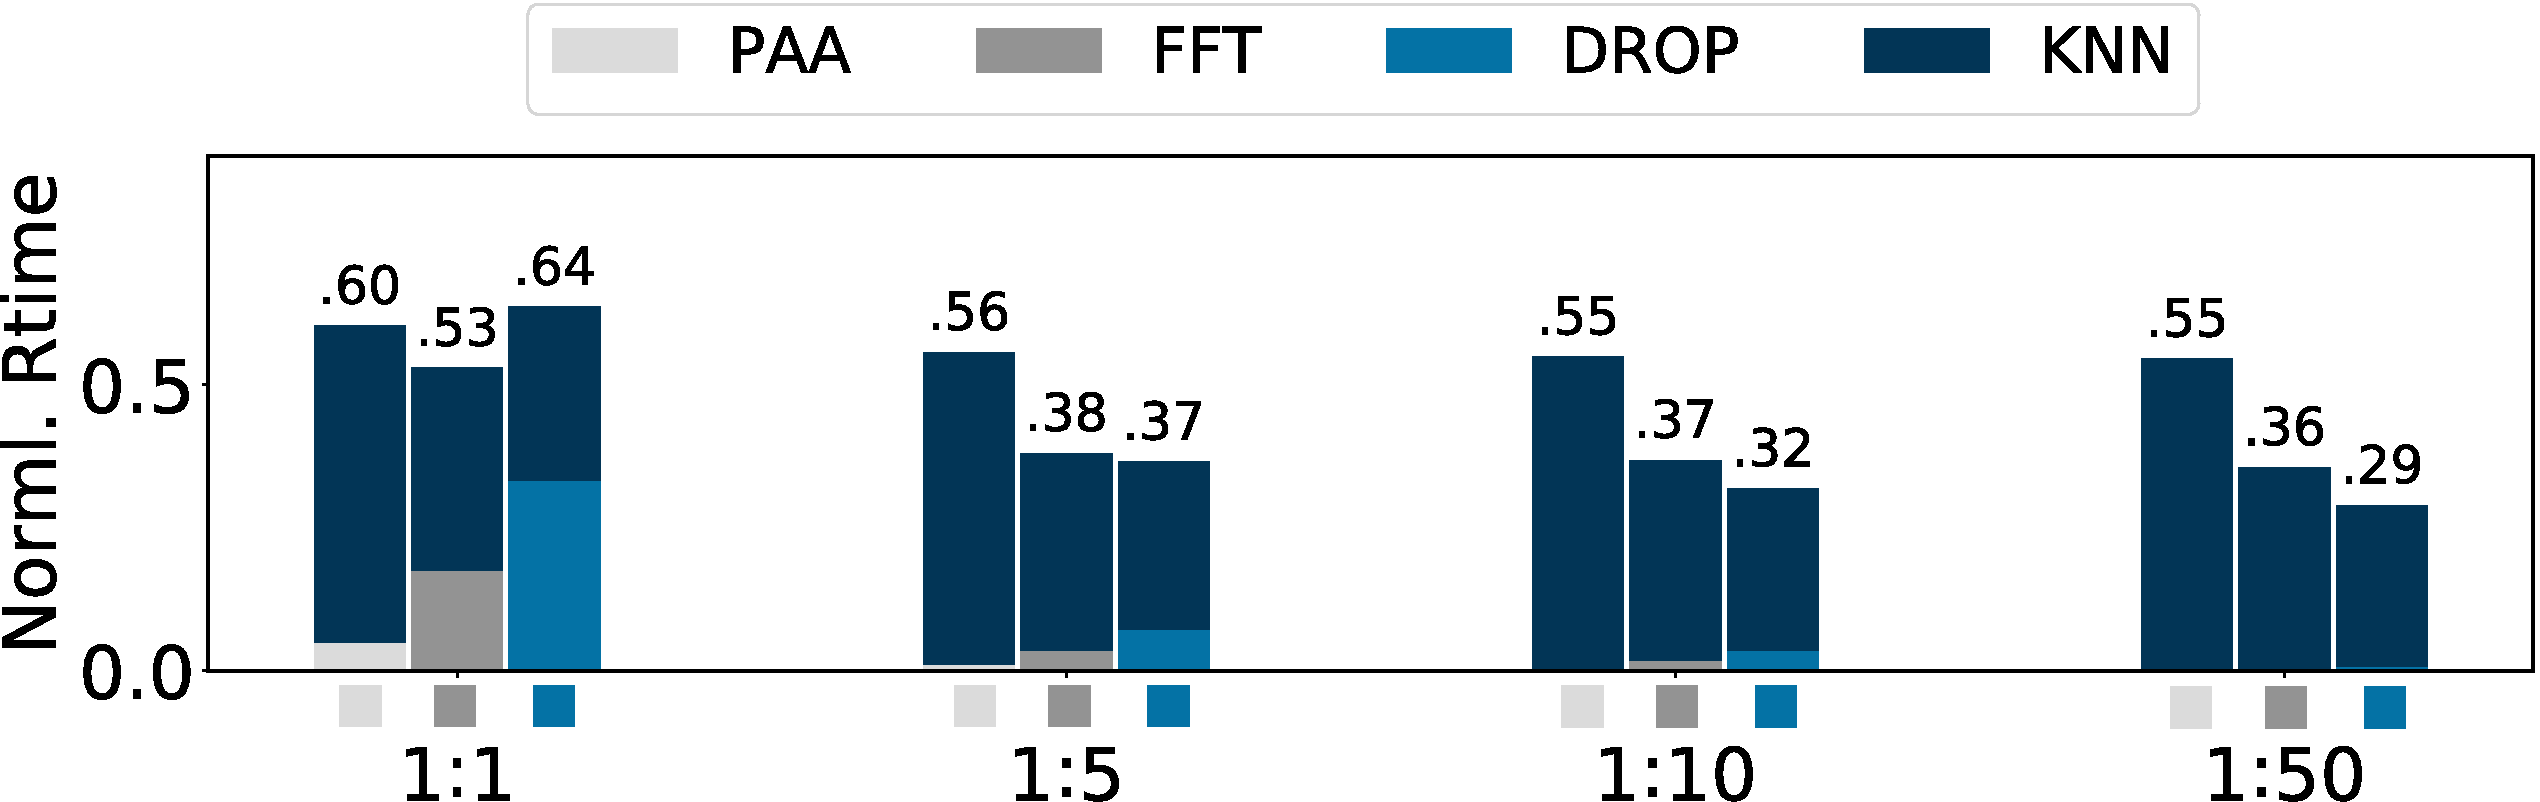
\includegraphics[width=\linewidth]{figs/query-rev.pdf}
\caption[]{Effect of decreasing the index-query ratio. As an index is queried more frequently, DROP's relative runtime benefit  increases.}
\label{fig:query}
\end{figure}

\red{
\minihead{Time Series Similarity Search Extensions}
Given the breadth of research in time series indexing, a natural question to ask is how DROP, a general operator for PCA, compares to state-of-the-art time series indexes. 
As a preliminary evaluation, we consider iSAX2+~\cite{isax}, a state-of-the-art indexing tool  in a 1:1 index-query ratio setting, using a publicly available Java implementation~\cite{isaxcode}. 
While these indexing techniques also optimize for the low index-query ratio setting, we find index construction to be a large bottleneck in these workloads. 
For iSax2+, index construction is on average $143\times$ (up to $389\times$) slower than DR via DROP, but is on average only $11.3\times$ faster than k-NN on the reduced space.  However, given high enough query workload, these specialized techniques will surpass DROP.


We also verify that DROP is able to perform well when using downstream similarity search tasks relying on alternative distance metrics, namely, Dynamic Time Warping (DTW)---a commonly used distance measure in the literature~\cite{isaxorig}. 
As proof-of-concept, we implement a 1-NN task using DTW with a 1:1 index-query ratio, and find that even with this high ratio, DROP provides on average $1.2\times$ and $1.3\times$ runtime improvement over PAA and FFT, respectively.
%As DTW is known to be incredibly slow~\cite{dtwslow}, it is unsurprising that DROP provides large runtime benefits for tasks using DTW without additional pruning---in terms of absolute runtime, DROP saves 2.8 minutes on the FordA dataset compared to PAA, and 2.2 minutes on the wafer dataset compared to FFT.


%Finally, as the considered time series are fairly short, we perform the same experiment over a standard gaussian random walk synthetic dataset~\cite{coconut,ssh} consisting of 50,000 time series of dimension 10,000. 
%Each time series is generated by, for each time step, generating a random value distributed via standard normal distribution, and adding it to the running sum of all previous time steps. 
%We find that DROP takes 4150ms to complete, whereas PAA and FFT take 5523ms (1.3$\times$ faster) and 15329ms (3.7$\times$ faster), respectively. 
}


\subsection{Lesion Study}
\label{subsec:lesion}


We perform a factor analysis of the incremental runtime and dimensionality contributions of each of DROP's components compared to baseline SVD methods. 
We only display the results of k-NN with cover trees; the results hold for the other indexes.
We use a 1:1 index-query ratio \red{with data inflated by 5$\times$} to better highlight the effects of each contribution to the DR routine, and display average results over the UCR datasets in Figure~\ref{fig:lesion}, excluding Phoneme.


\begin{figure}
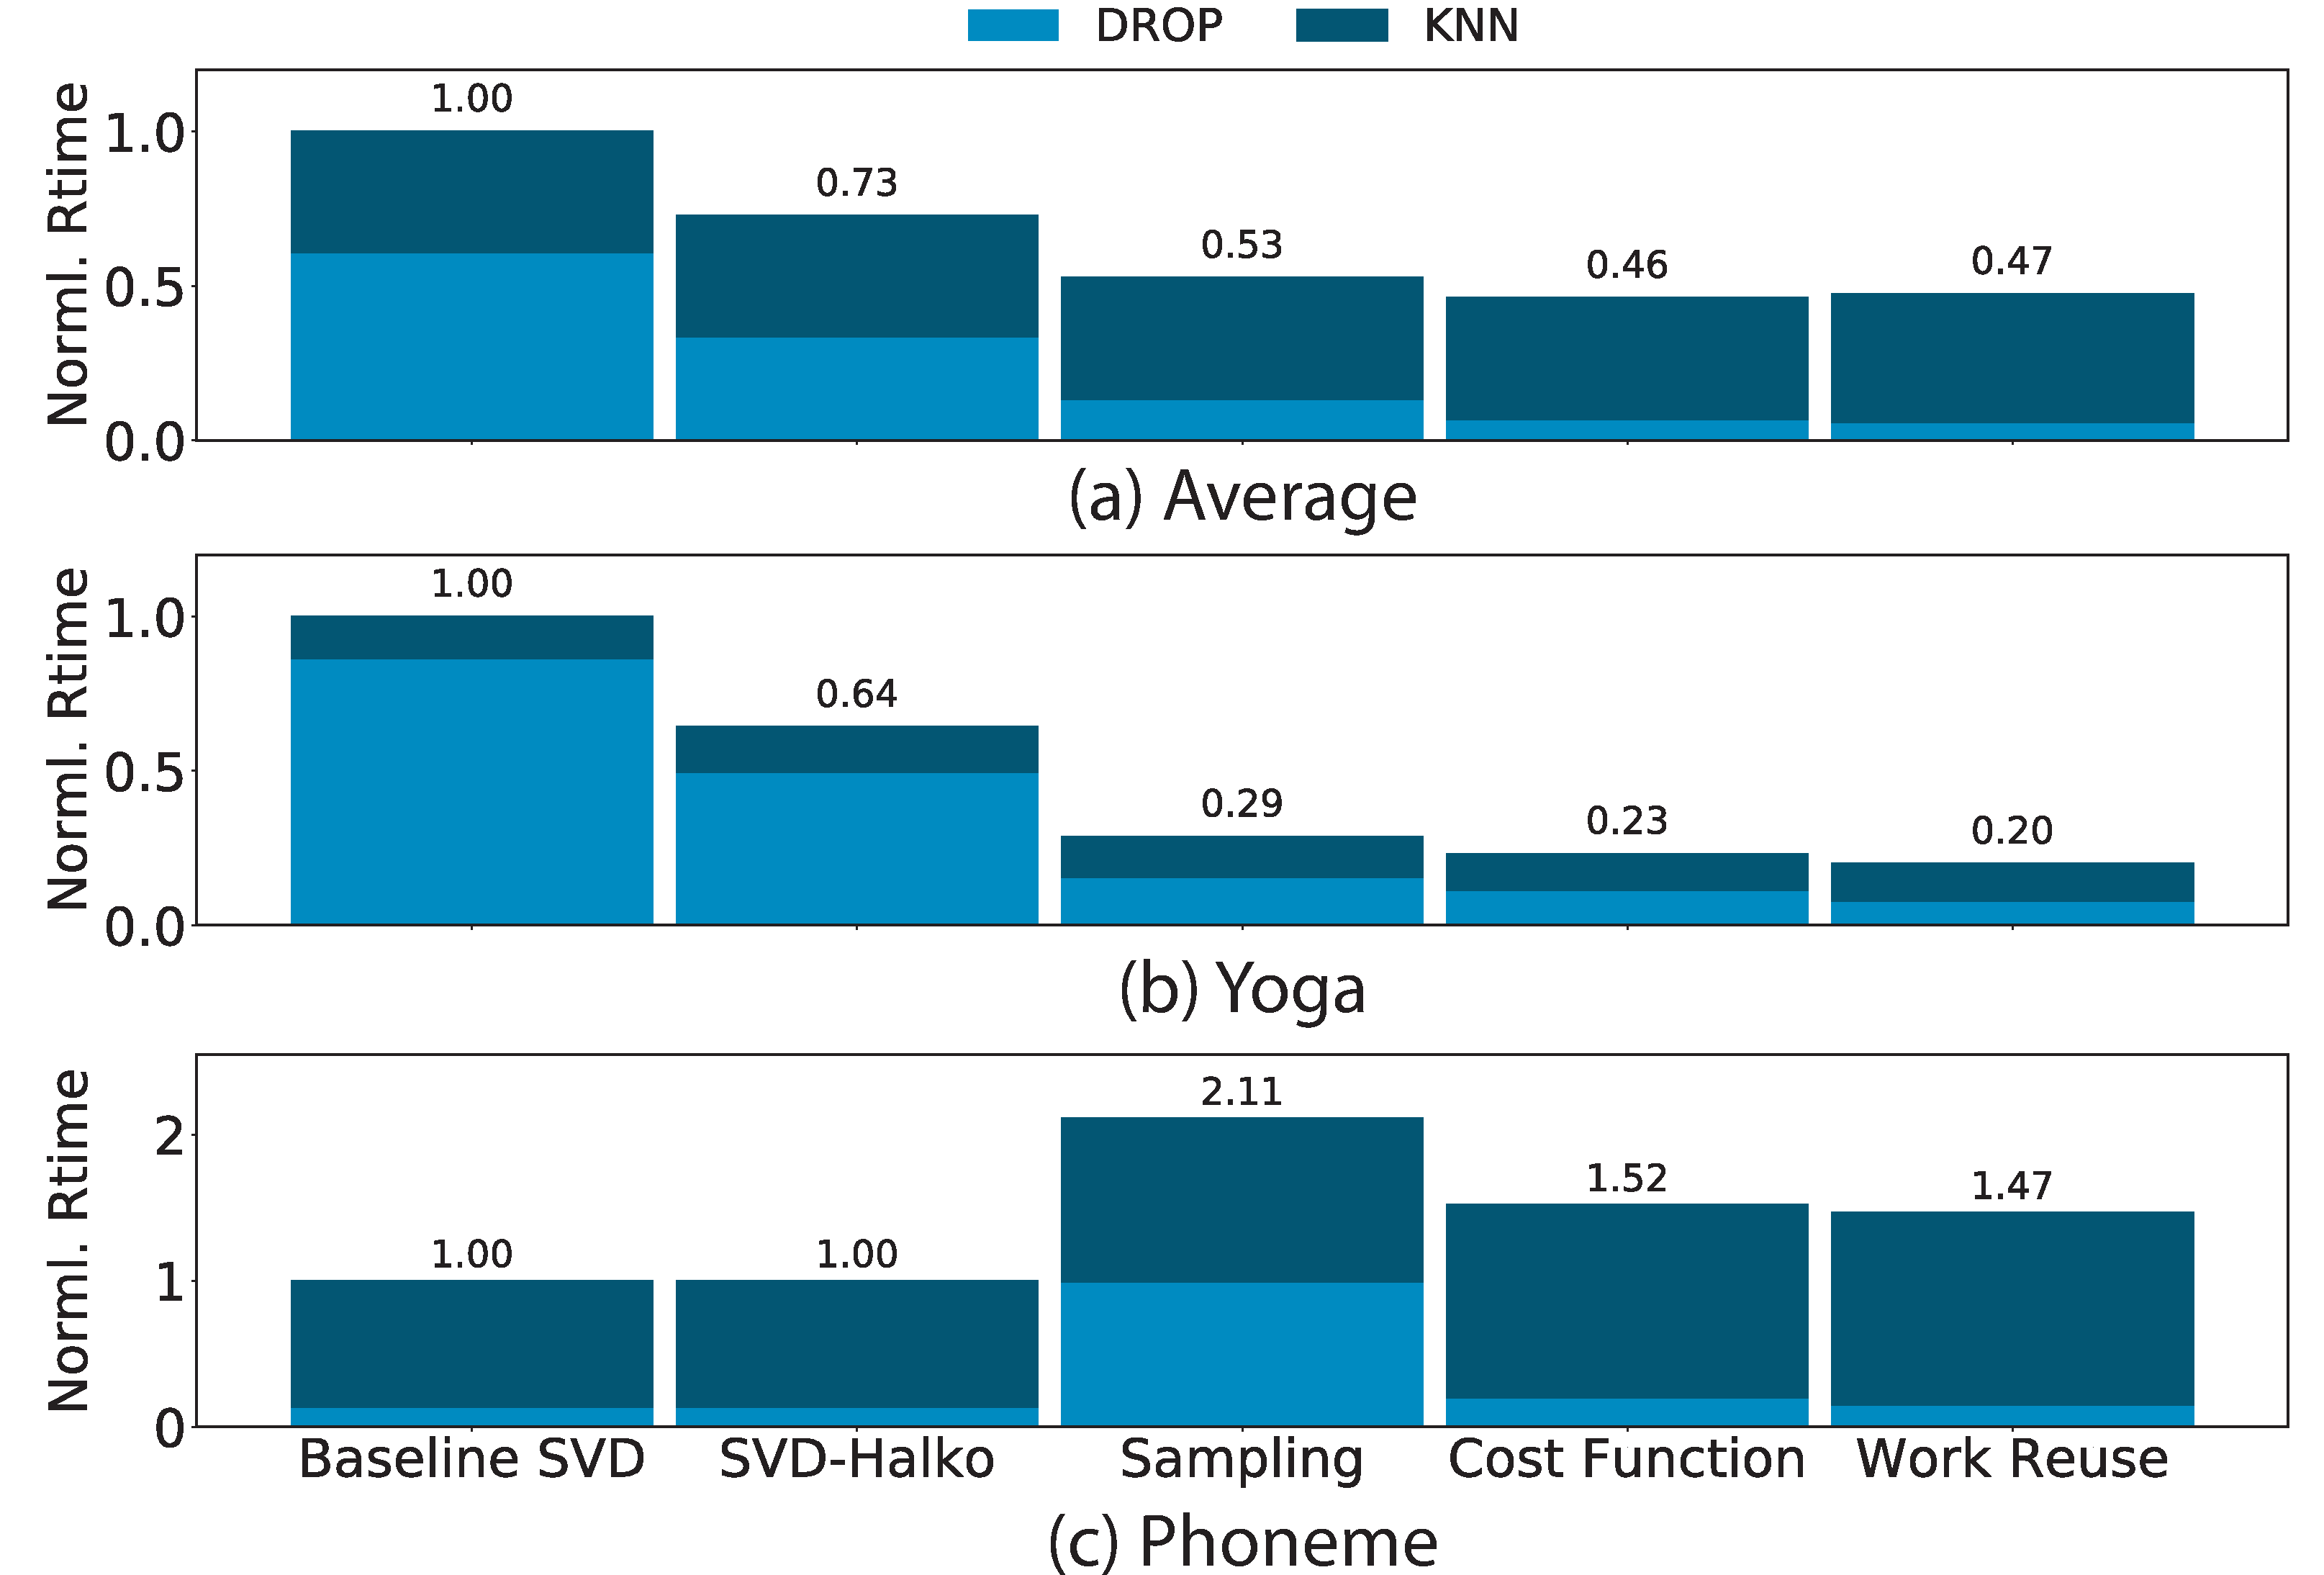
\includegraphics[width=\linewidth]{figs/lesion-all.pdf}
\caption[]{Lesion studies over the UCR datasets.}
\label{fig:lesion}
\end{figure}

Figure~\ref{fig:lesion} first demonstrates the boost from using SVD-Halko over a na\"ive implementation of PCA via SVD, which comes from not computing the full transformation a priori, incrementally binary searching as needed. 
It then shows the runtime boost obtained from running on samples until convergence, where DROP samples and terminates after the returned lower dimension from each iteration plateaus.
This represents the na\"ive sampling-until-convergence approach that DROP defaults to sans user-specified cost model.
We finally introduce cost based optimization and work reuse.
Each of these optimizations improves runtime, with the exception of work reuse, which has a negligible impact on average but disproportionately impacts certain datasets. 

\begin{comment}
\red{On average, DROP is $2.1\times$ faster (up to $41\times$) than PCA via SVD, and $1.6\times$ faster than SVD-Halko (up to $3.3\times$). DROP with cost-based optimization is faster than  sampling to convergence by $1.2\times$ on average, but this default strategy is still $1.4\times$ faster than SVD-Halko on average.}


\begin{comment}
\begin{figure}
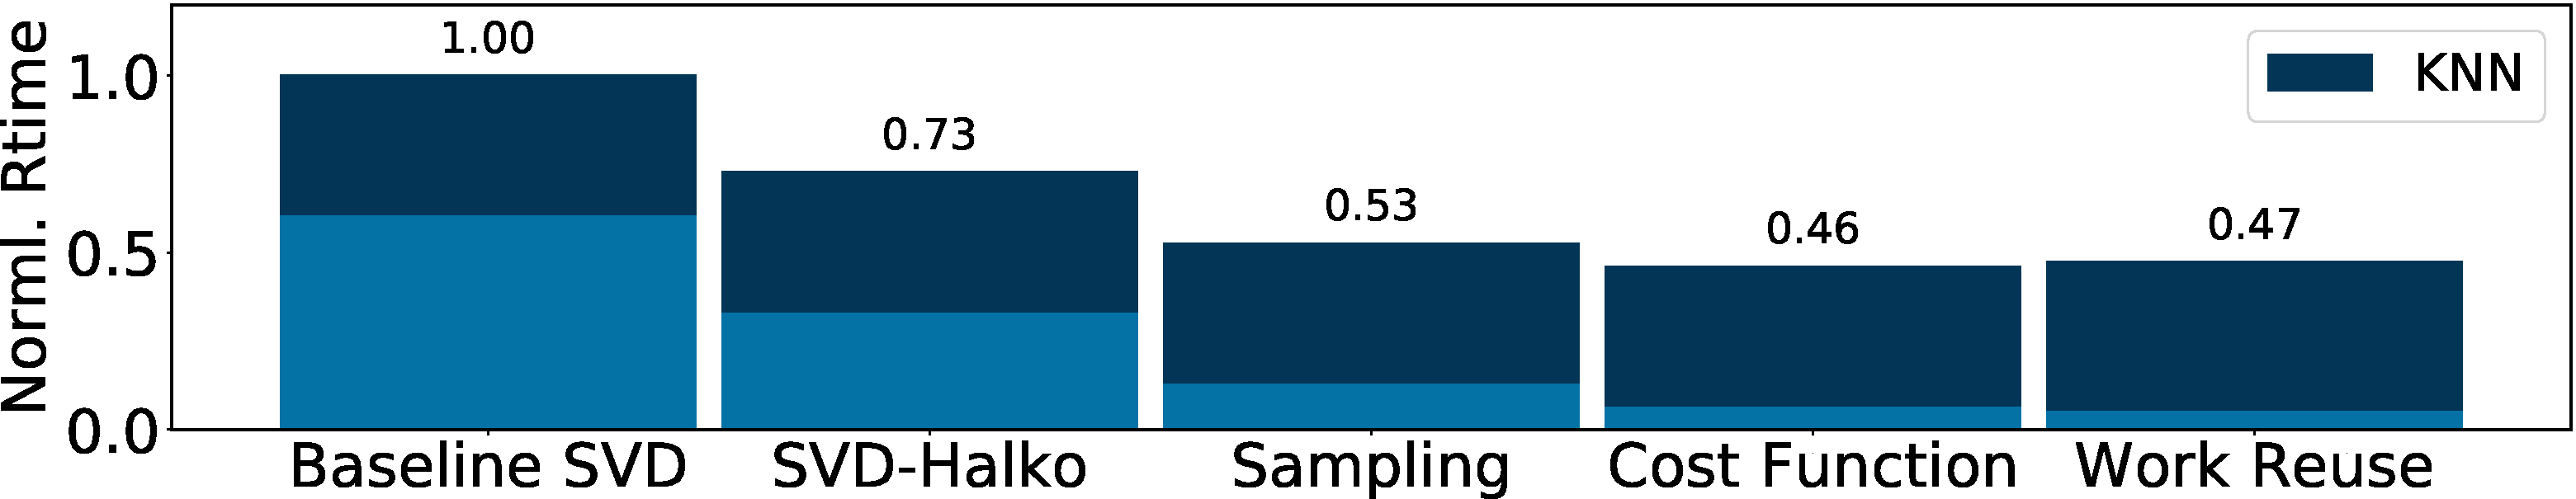
\includegraphics[width=\linewidth]{figs/lesion-rev.pdf}
\caption[]{Average result of lesion study over the UCR datasets.}
\label{fig:lesion}
\end{figure}

\begin{figure}
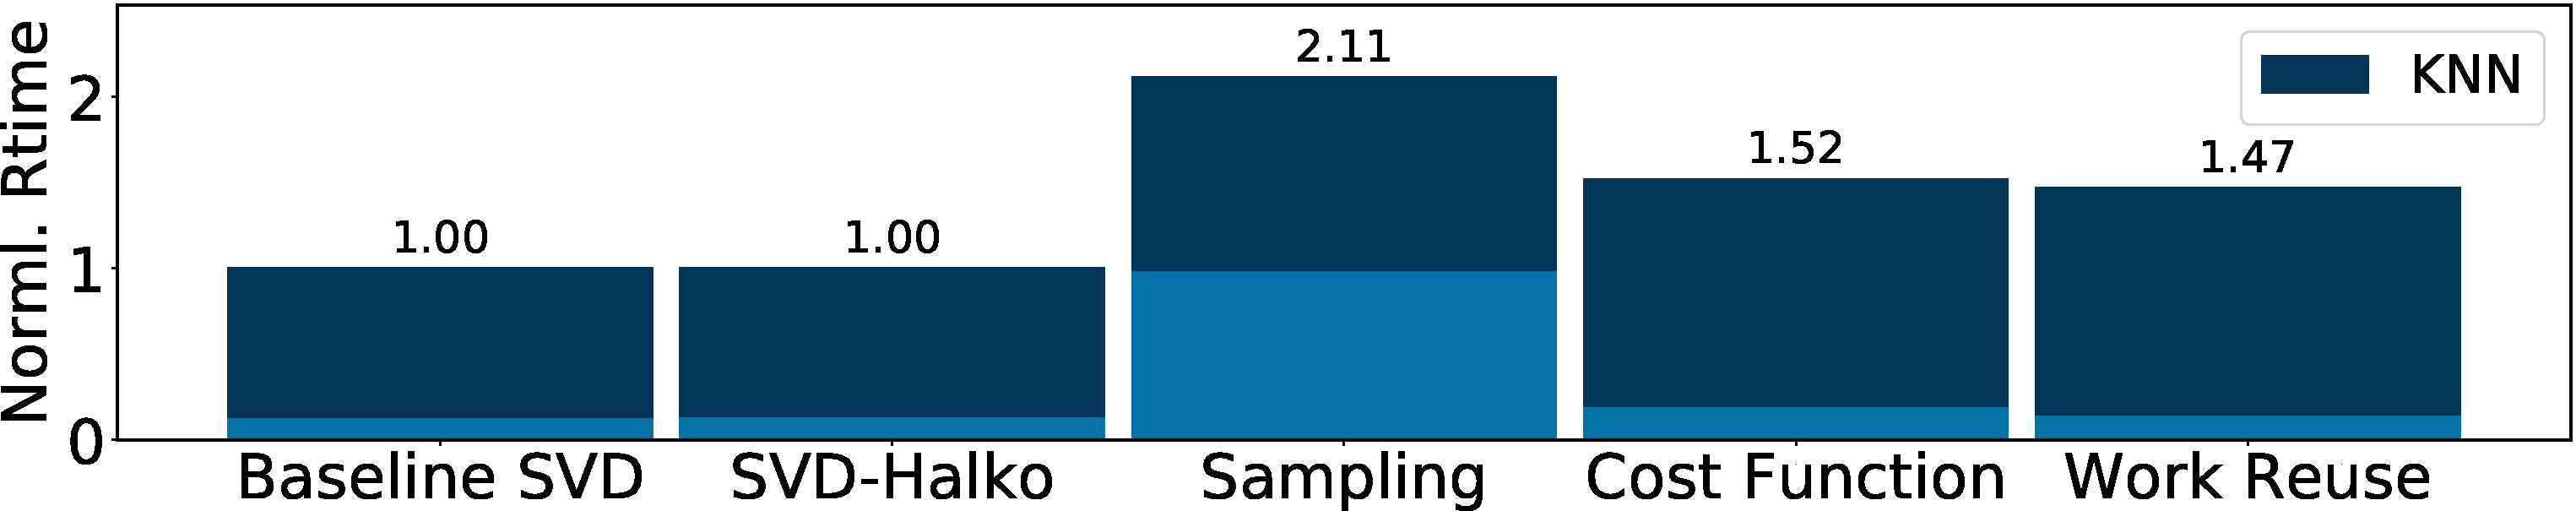
\includegraphics[width=\linewidth]{figs/phoneme-rev.pdf}
\caption[]{Lesion study of the UCR phoneme, a dataset with high intrinsic dimensionality, meaning sampling to convergence is orders of magnitude slower than a batch SVD. DROP's cost function enables it to terminate in advance, returning a higher dimensional basis to minimize reduce overall compute.}
\label{fig:phoneme_lesion}
\end{figure}

\begin{figure}
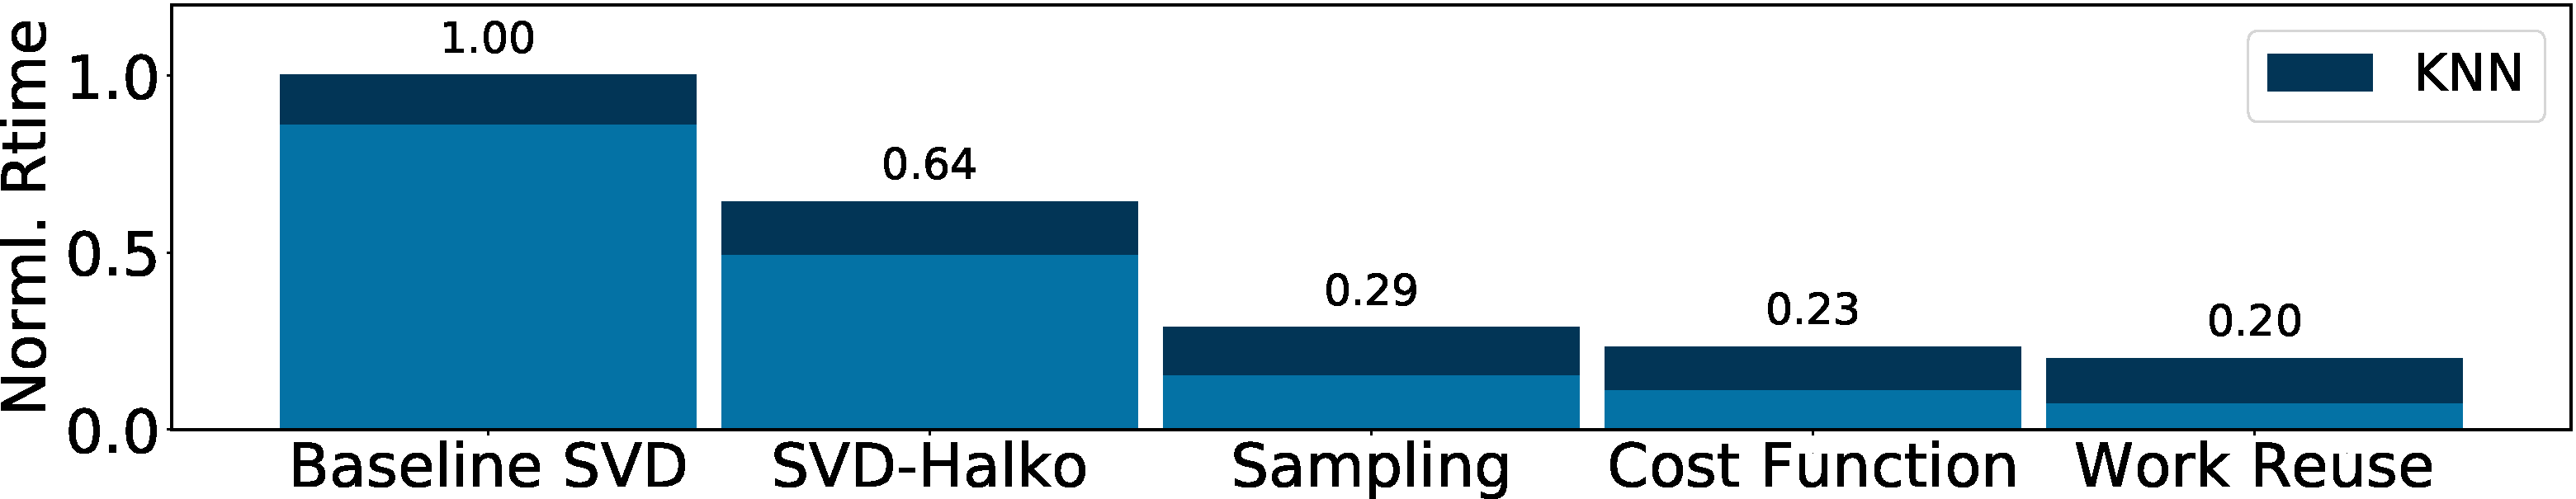
\includegraphics[width=\linewidth]{figs/yoga-rev.pdf}
\caption[]{Lesion study over the UCR yoga dataset. Work reuse provides a $15\%$ runtime improvement.}
\label{fig:yoga-lesion}
\end{figure}
\end{comment}

Work reuse typically only slightly affects end-to-end runtime as it is useful primarily when a large number of DROP iterations are required.
We also observe this behavior on certain small datasets with moderate intrinsic dimensionality, such as the yoga dataset in Figure~\ref{fig:lesion}b. 
Work reuse provides a $15\%$ improvement in addition to cost based optimization.

DROP's sampling operates on the premise that the dataset has data-point-level redundancy. 
However, datasets without this structure are more difficult to reduce the dimensionality of.
Phoneme is an example of one such dataset (Figure~\ref{fig:lesion}c).  
In this setting, DROP \red{incrementally examines a large proportion of data before enabling cost-based optimization,} resulting in a performance penalty.
%We discuss extensions to DROP to mitigate this in the extended version of this manuscript. 

%Section~\ref{subsec:disc}.%, and provide all lesion studies in the Appendix.



\begin{comment}
\subsection{Scalability}
\label{subsec:scale}
Data generated by automated processes such as time series often grows much faster in size than intrinsic dimensionality.
DROP can exploit this intrinsic dimensionality to compute PCA faster than traditional methods as it only processes an \emph{entire} dataset if a low intrinsic dimensionality does not exist. 

To demonstrate this, we fix intrinsic dimensionality of a synthetic dataset generated via random projections to 8 as we grow the number of datapoints from 5K to 135K. 
Hence, the sample size an algorithm requires to uncover this dataset's intrinsic dimensionality is constant regardless of the full dataset size. 
In this experiment, we enable DROP's fixed-size sampling schedule set to increase by 500 datapoints at each iteration. 
As Figure~\ref{fig:increasingdata} shows, DROP is able to find a 8-dimensional basis that preserves $TLB$ to $0.99$ within \red{145ms} for dataset sizes up to 135K data points, and is \red{$12\times$} faster than binary search with SVD-Halko. 
Runtime is near constant as dataset size increases, with small overhead due to sampling from larger datasets.
This near-constant runtime contrasts with PCA via SVD and SVD-Halko as they do not exploit the intrinsic dimensionality of the dataset and process all provided points, further illustrating the scalability and utility of sample-based DR.


\begin{figure}
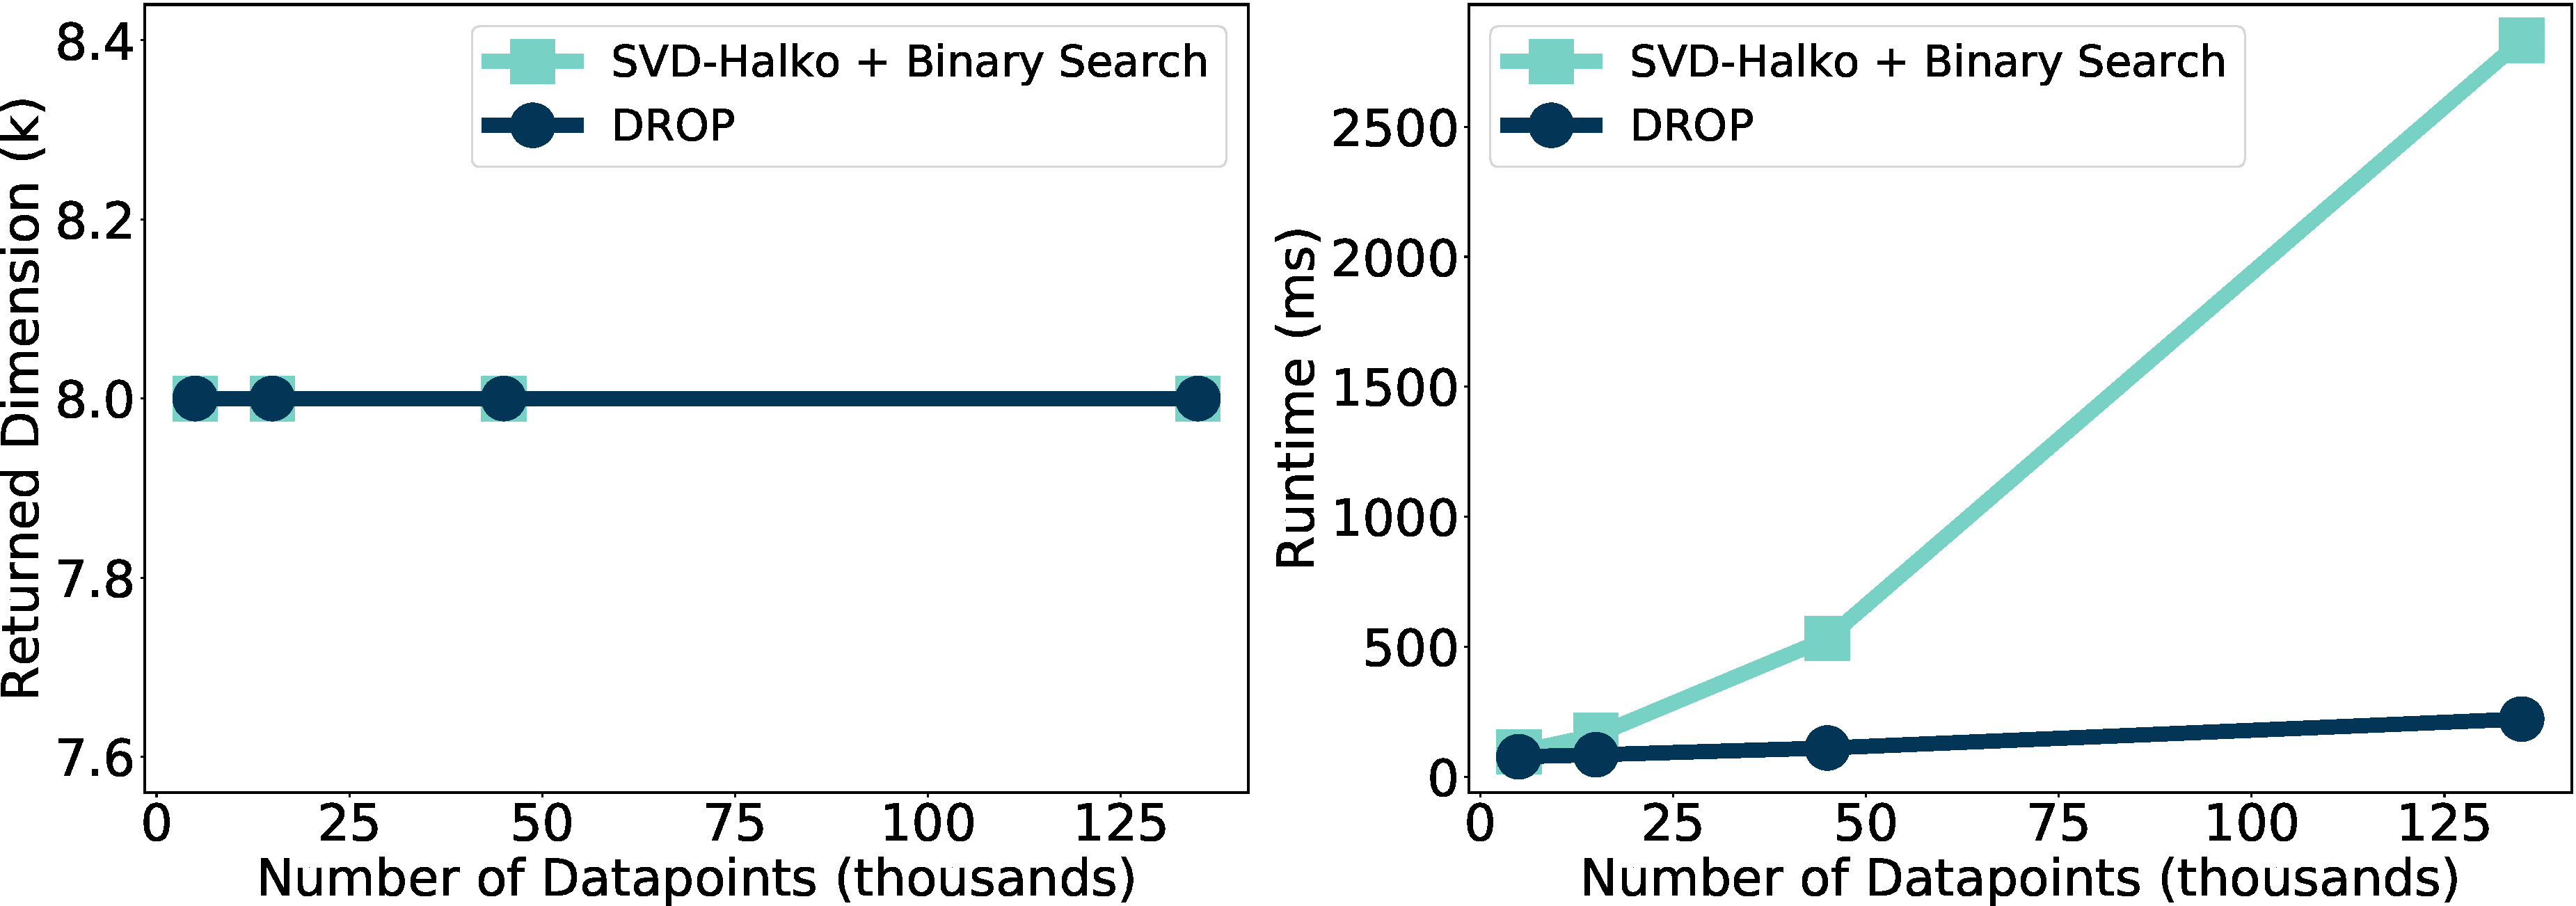
\includegraphics[width=\linewidth]{figs/increasing-revision.pdf}
\caption[]{Effect of dataset size on time and output dimension ($k$), with constant intrinsic data dimensionality of 8. DROP runtime with a fixed schedule remains near constant.}
\label{fig:increasingdata}
\end{figure}

\end{comment}


\begin{figure}
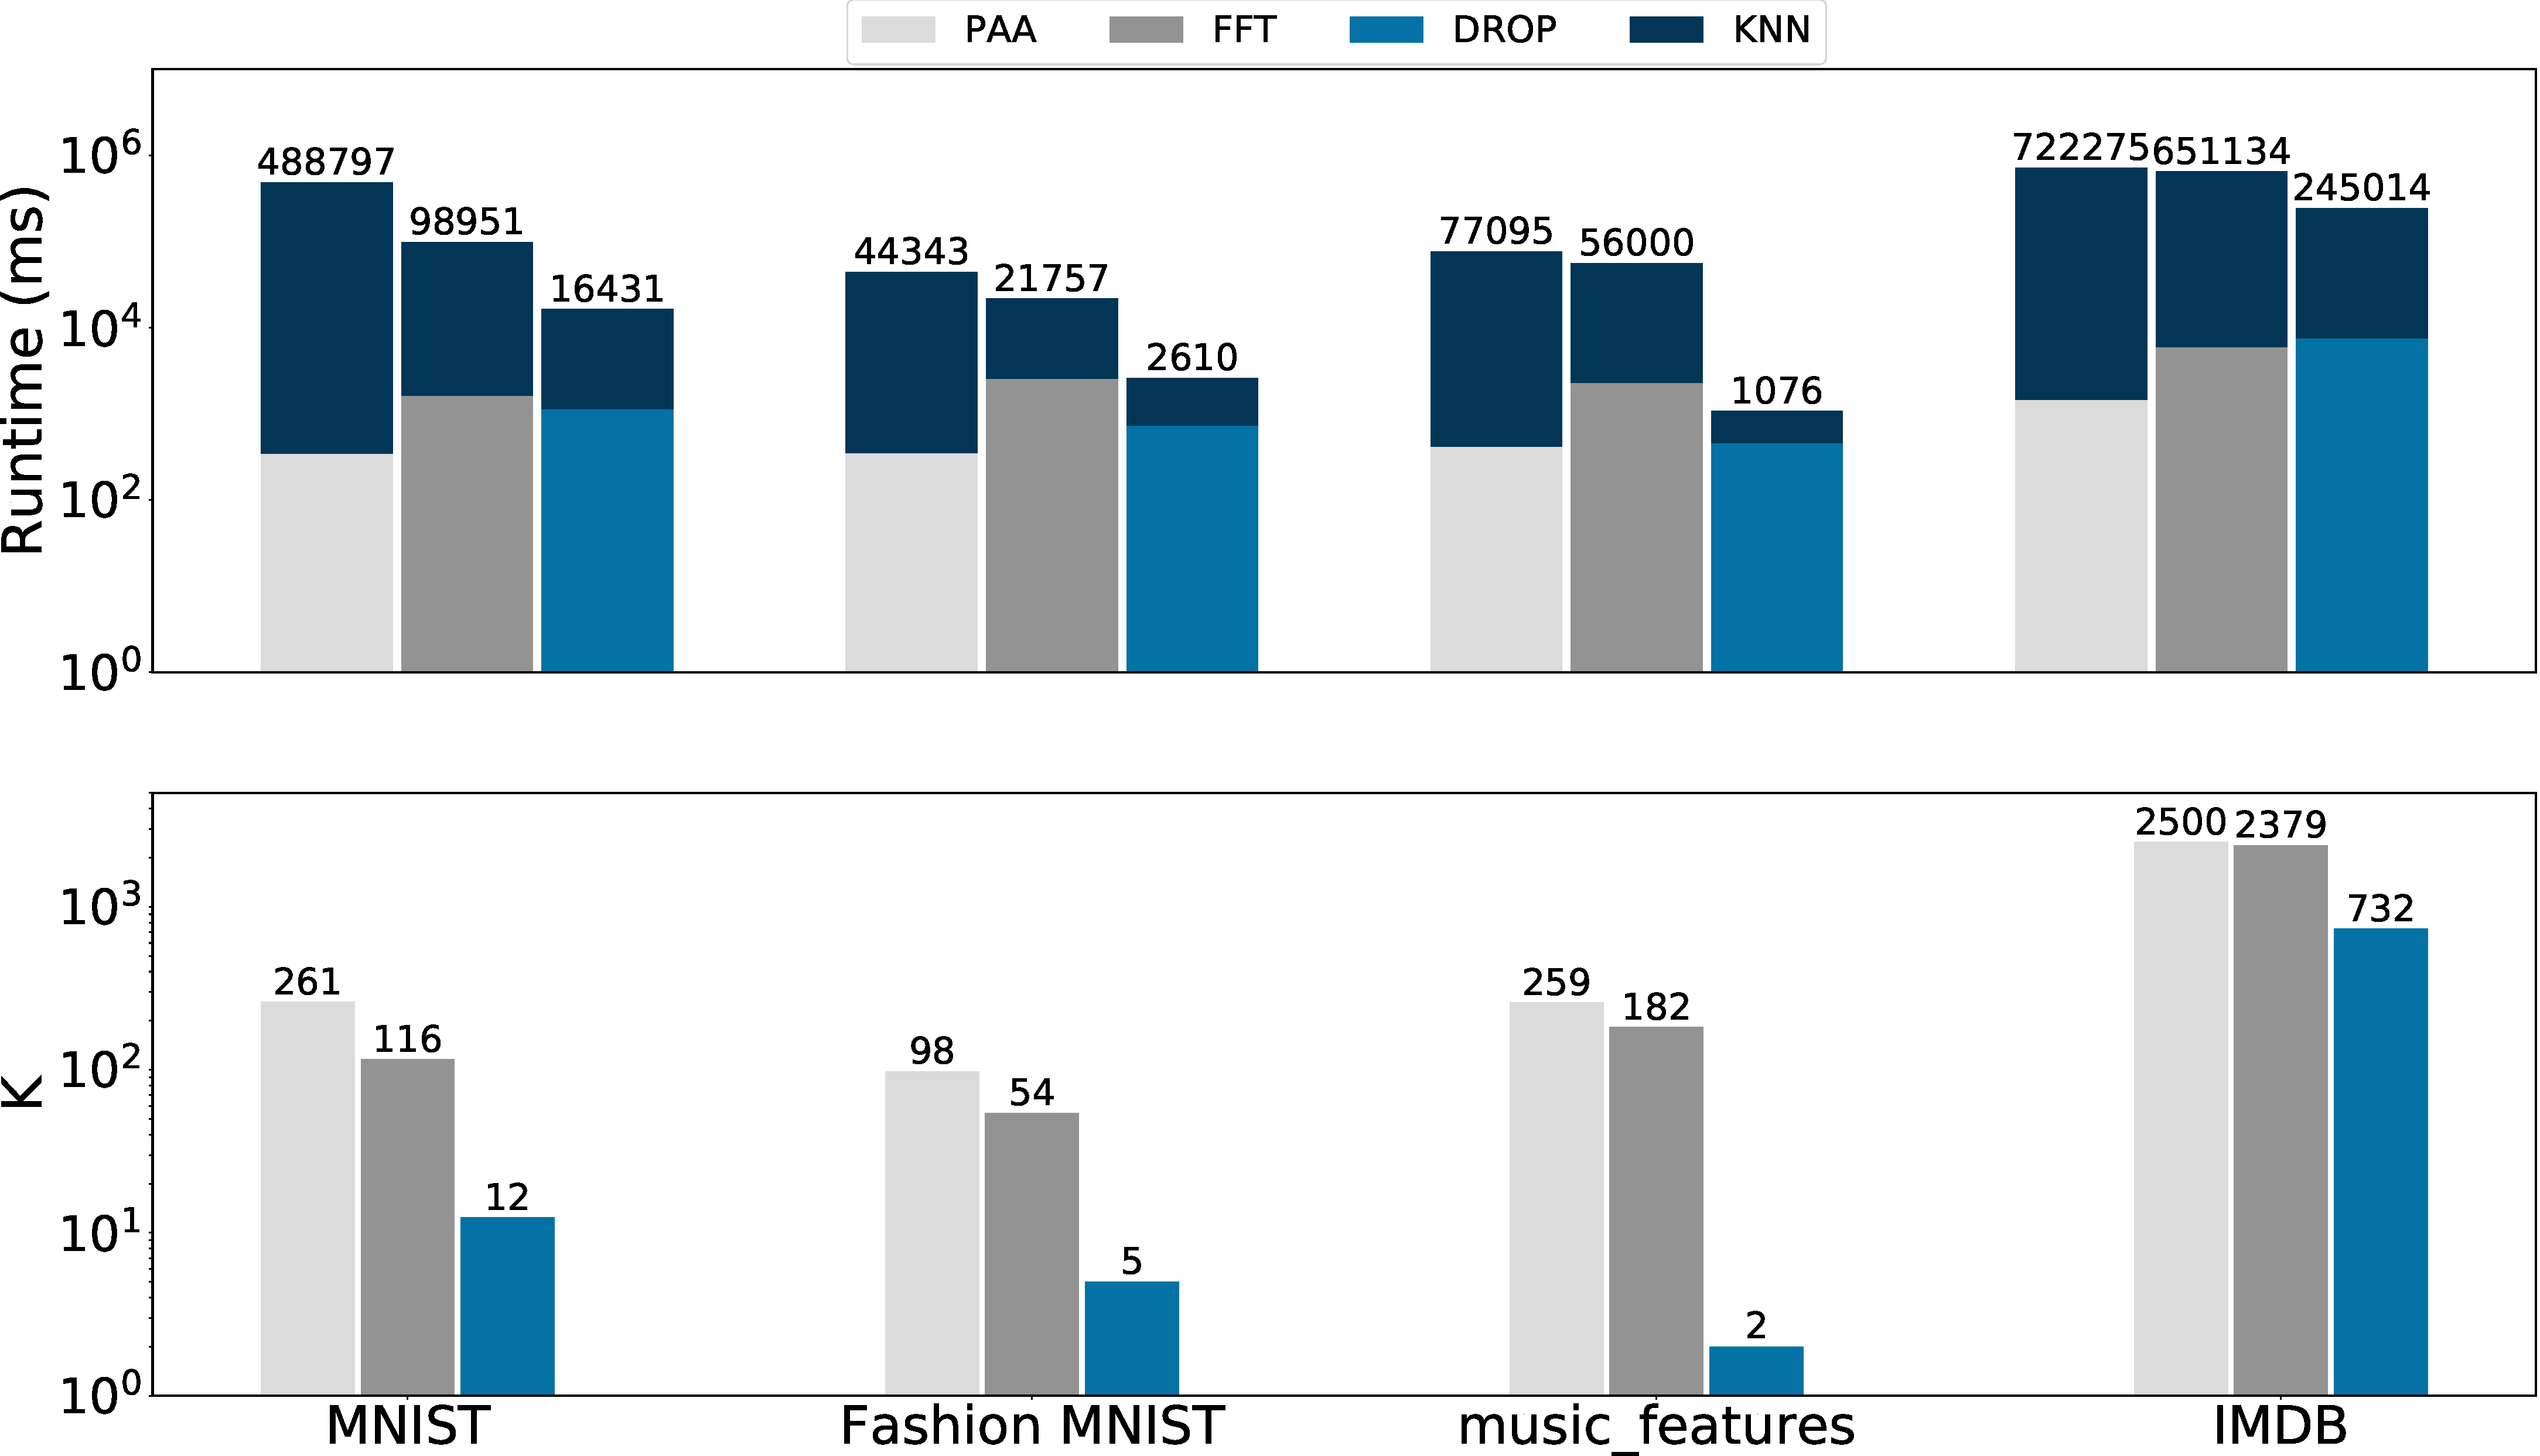
\includegraphics[width=\linewidth]{figs/nonts-revision.pdf}
\caption[]{End-to-End k-NN runtime (top) and returned dimension $k$ (bottom) over the entire MNIST dataset and the FMA featurized music dataset.}
\label{fig:beyond}
\end{figure}

\red{
\subsection{Beyond the Time Series Case Study}
\label{subsec:nonts}

We consider generalizability beyond our initial case study along two axes: data domain and downstream workload. These preliminary results show promise in extension to additional domains and target tasks.  

\subsubsection*{Data Domain}
We examine classification/similarity search workloads across  image classification, music analysis, and natural language processing. 
}
To better show the trade-off in DR and downstream workload, we repeat the k-NN retrieval experiments with a 1:1 index-query ratio.
We use the MNIST hand-written digit image dataset containing 70,000 images of dimension 784 (obtained by flattening each $28 \times 28$-dimensional image into a single vector~\cite{mnist}, combining both the provided training and testing datasets); FMA's featurized music dataset, providing  518 features across 106,574 music tracks; a bag-of-words representation of an IMDB sentiment analysis dataset across 25,000 movies with 5000 features~\cite{imdb}; \red{Fashion MNIST's 70,000 images of dimension 784~\cite{fashion}}.  
We present our results in Figure~\ref{fig:beyond}.
As the given datasets are larger than the ones presented in~\cite{ucr}, DROP's ability to find a $TLB$-preserving low dimensional basis is more valuable as this more directly translates to significant reduction in end-to-end runtime---up to \red{a 7.6 minute wall-clock improvement in MNIST, 42 second improvement in Fashion MNIST, 1.2 minute improvement in music features, and 8 minute improvement in IMDB compared to PAA. 
These wall-clock runtime effects will only be amplified as the index-query ratio decreases, to be more typical of the repeated-query setting. 
For instance, when we decrease the ratio to 1:5 on the music features dataset, DROP provides a 6.1 and 4.5 minute improvement compared to PAA and FFT, respectively. 
}

\red{
\subsubsection*{Downstream Workload}
To demonstrate the generalizability of both DROP's pipeline as well as black-box runtime cost-model estimation routines, we extend our pipeline to perform a k-means task over the MNIST digits dataset. 
We fit a new downstream workload runtime model as we did with k-NN, and operate under a 1:1 index-query ratio. 
In this workload, DROP terminates in 1488ms, which is 16.5$\times$ faster than PAA and 6.5$\times$ faster than FFT. 
}



\begin{comment}
\subsection{PCA Subroutine Evaluation}
\label{subsec:pcaexp}

PCA algorithms  are optimized for different purposes, with varying convergence, runtime, and communication complexity guarantees. 
DROP is agnostic to choice of PCA subroutine, and improvements to said routine provide complementary runtime benefits. 
\red{To implement DROP's default algorithm, we use MTJ and netlib-java linked against Intel MKL. 
Our SVD subroutine is competitive with the commonly used SciPy library~\cite{scipy} in Python linked against Intel MKL. 
We provide a plot of the runtimes over the UCR datasets (original, and number of datapoints inflated by $5\times$).

We also provide implementations of PCA via SMILE, Probabilistic PCA via SMILE's implementation, and PCA via (stochastic) Oja's method (not linked against Intel MKL) as a proof-of-concept of DROP's modularity, but they perform orders of magnitude slower than the optimized default.}



\begin{figure}
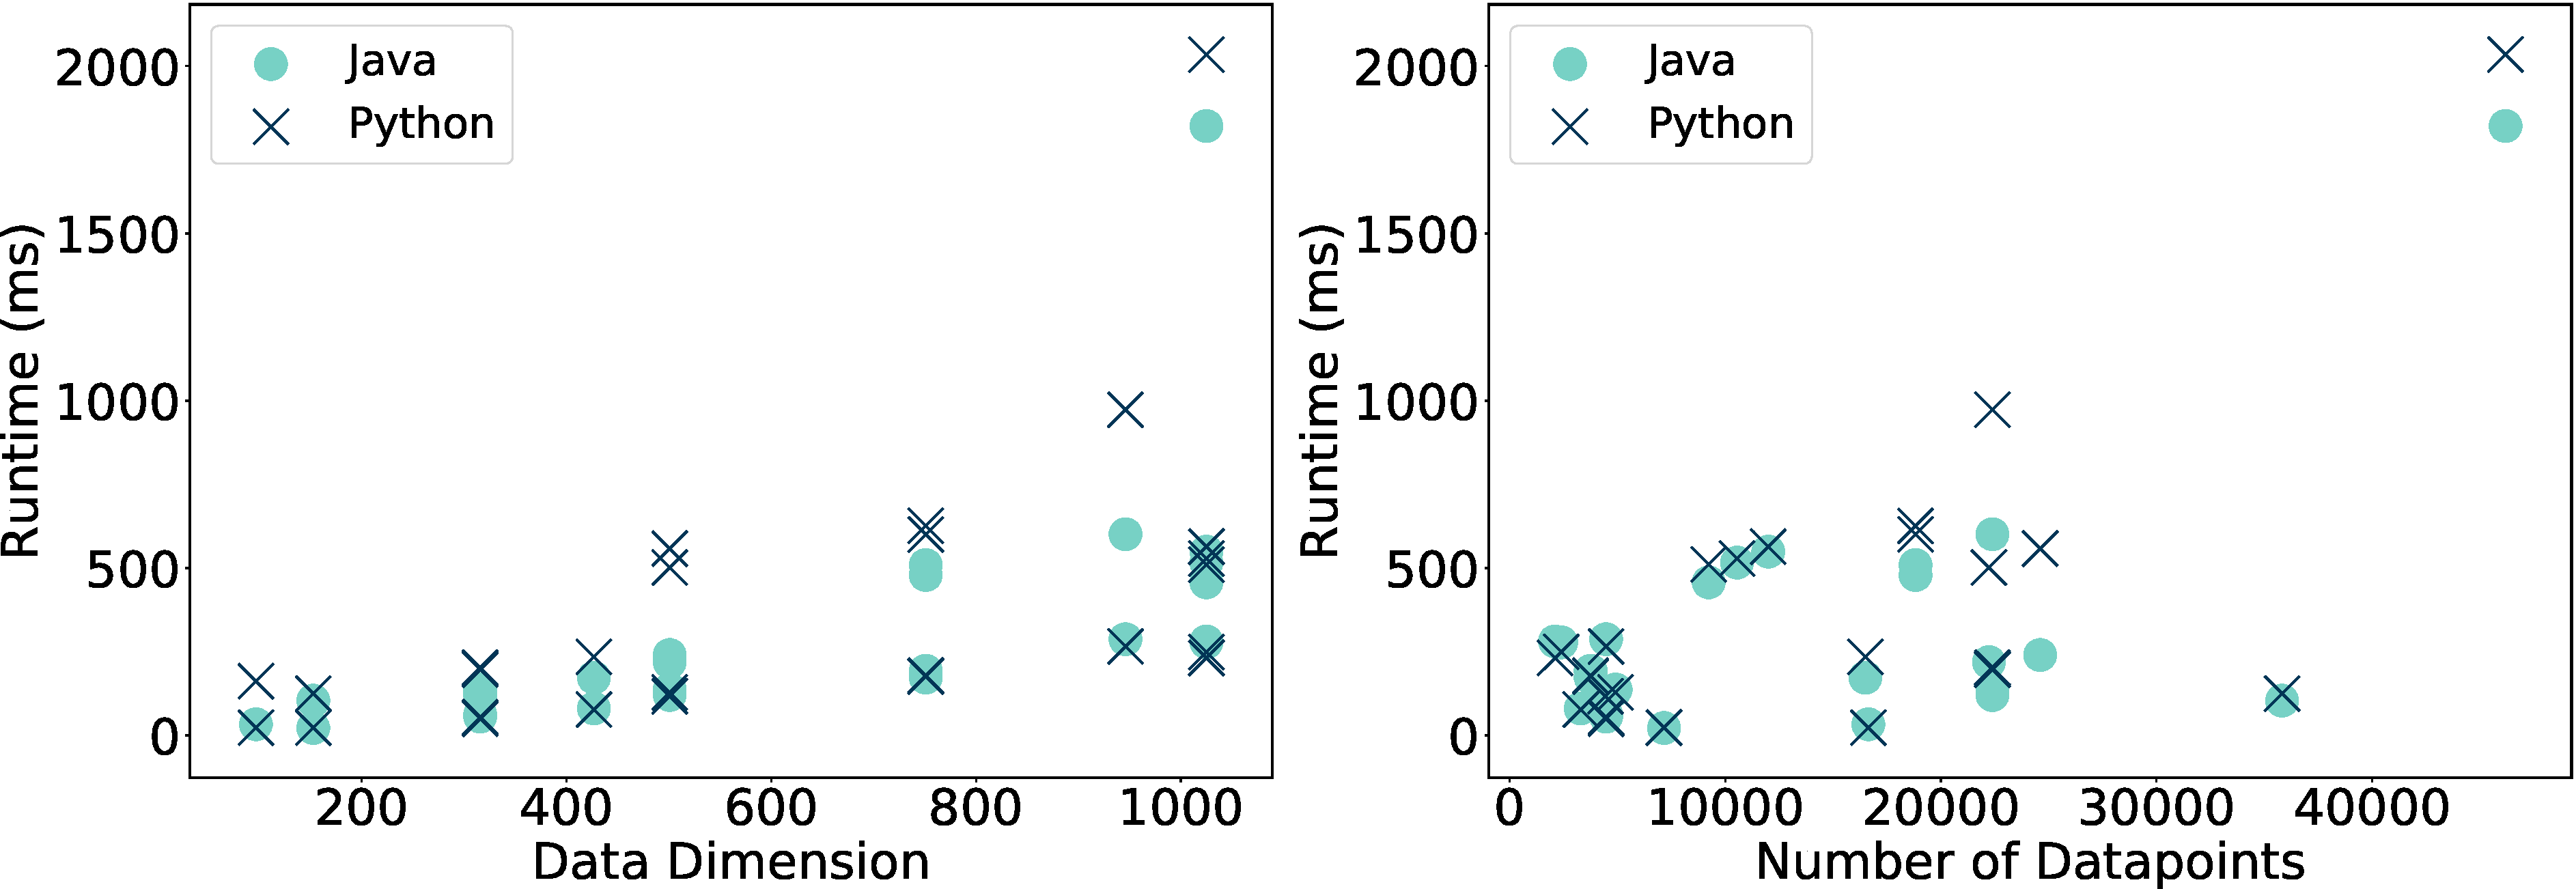
\includegraphics[width=\linewidth]{figs/runtime-revision.pdf}
\caption[]{Comparison of DROP's java PCA implementation with Python (SciPy) over the UCR datasets. }
\label{fig:pca_comp}
\end{figure}
\end{comment}






     

 

%\red{
\section{Future Work and Conclusions}
\label{subsec:disc}

%\subsection{Generalization}
%The techniques introduced via DROP can benefit any repeated-query setting where PCA is the method of choice, so long as users are willing to sacrifice small amounts of accuracy for improved running time and a metric of interest can be defined for the application (i.e., $TLB$ for similarity search, or loss function estimates for more general tasks). 
%For instance, examining a recent natural language processing application of PCA as a word vector post-processing step prior to downstream workloads~\cite{allbut} is exciting future work. 
%While having an exact runtime model is not common a priori, many common analytics workloads for clustering, classification, or regression, black-box techniques (as we used for k-NN and k-means) can be applied as downstream tasks can be performed as a series of matrix decompositions and multiplies (i.e., techniques that make use of gradient descent). 
%}
DROP provides a first step in bridging the gap between quality and efficiency in DR for downstream \red{analytics}.
However, there are several avenues to explore for future work, such as sophisticated sampling methods and streaming execution.

\subsection{Data-Aware Sampling}
%We demonstrated that workload-aware approximate PCA can provide large end-to-end speedups in \red{our time series case study} and for non-time series datasets with low intrinsic dimensionality.

DROP's efficiency is determined by the dataset's spectrum; MALLAT, with the sharpest drop-off, performs extremely well, and Phoneme, with a near uniform distribution, does not.
Datasets such as Phoneme perform poorly under the default configuration as we enable cost-based optimization after reaching a feasible point.
Thus, DROP spends a disproportionate time sampling (Fig.~\ref{fig:phoneme_lesion}). 
Extending DROP to more efficiently determine if a dataset is amenable to aggressive sampling is an exciting area of future work. 
For instance, recent theoretical results that use sampling to estimate spectrum, even when the number of samples are small in comparison to the input dimensionality~\cite{estspec}, can be run alongside DROP with minimal alteration.

%To combat this, we provide an alternate sampling schedule that aggressively increases the sampling rate to quickly reach a $TLB$-achieving state if DROP repeatedly fails to meet the target $TLB$. 

%\vspace{.2cm}
%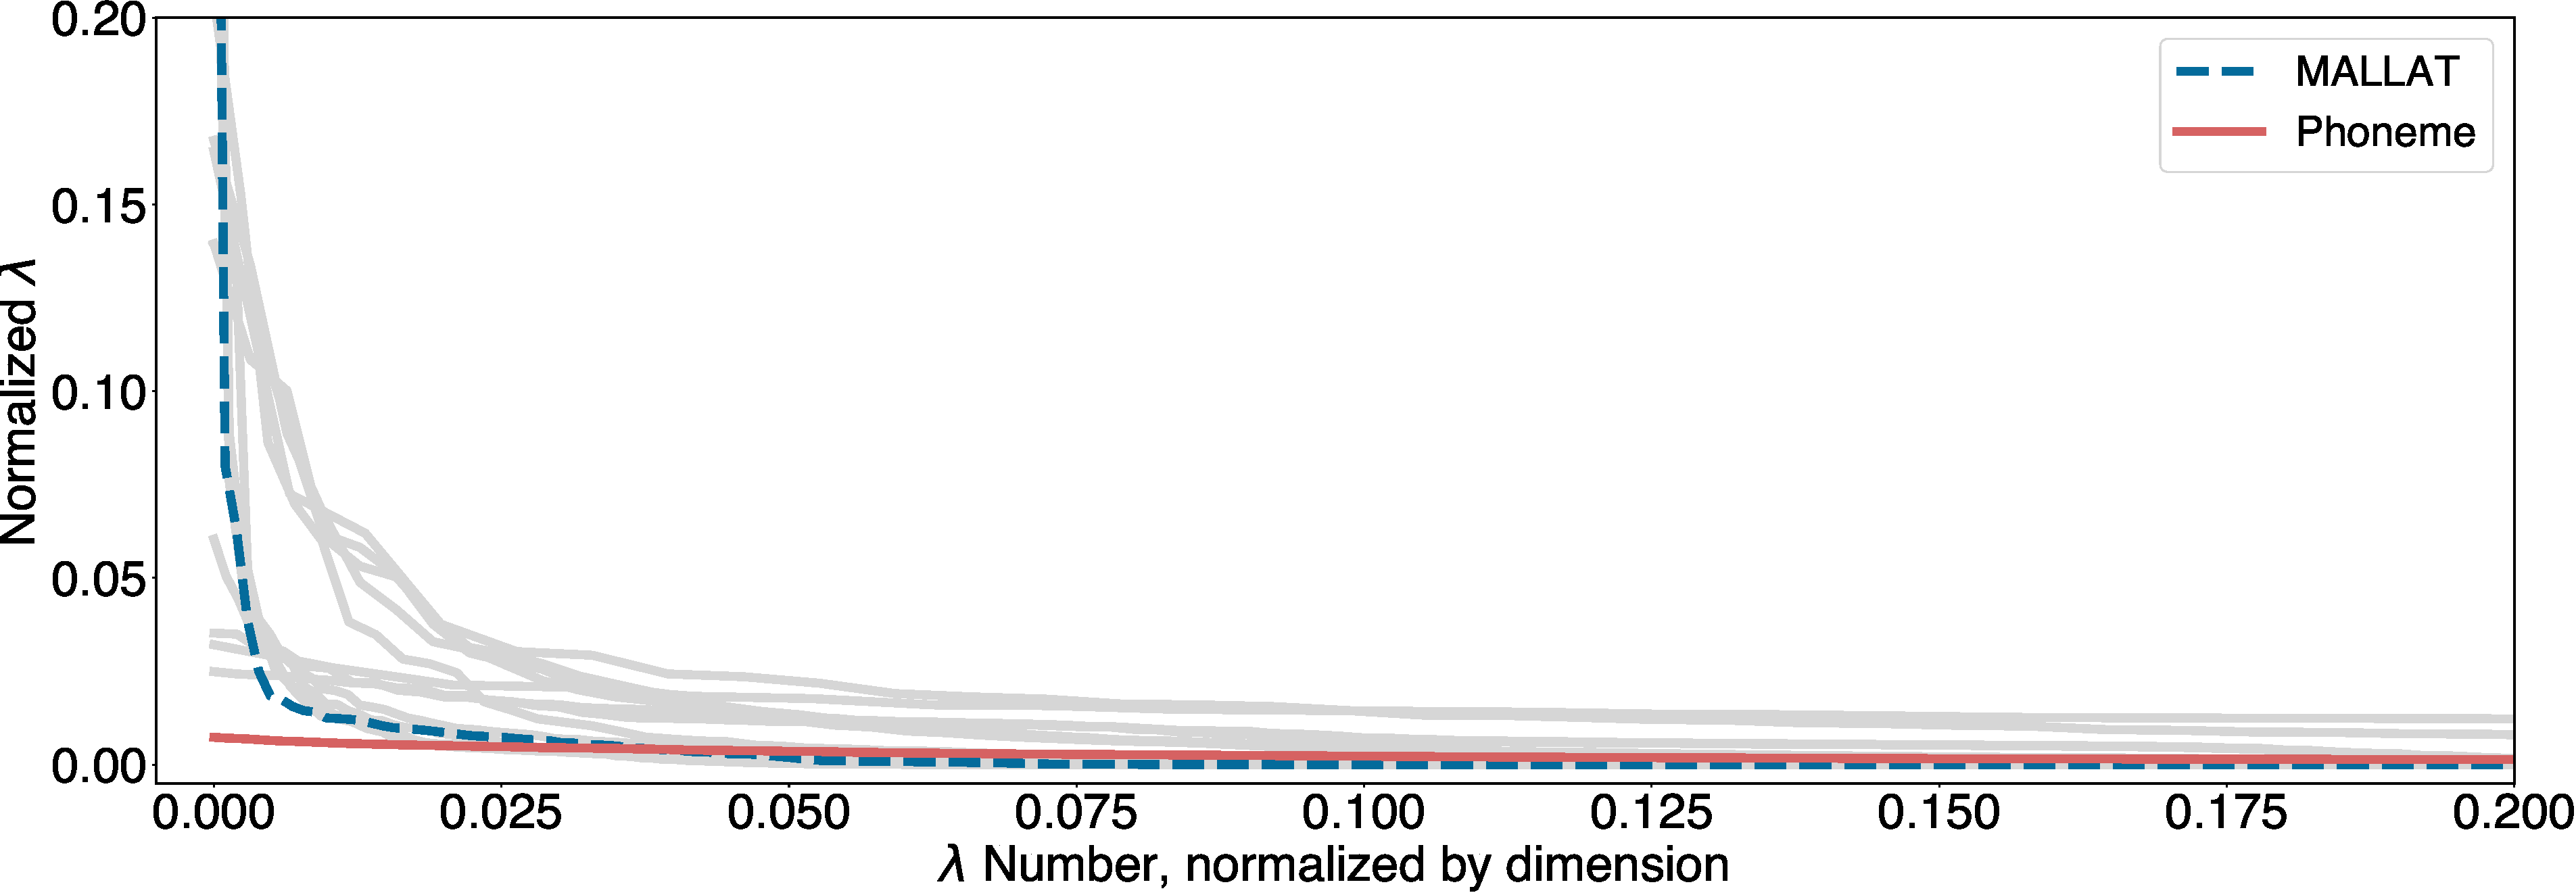
\includegraphics[width= .9\linewidth]{figs/spectrum-rev.pdf}

%\begin{figure}
%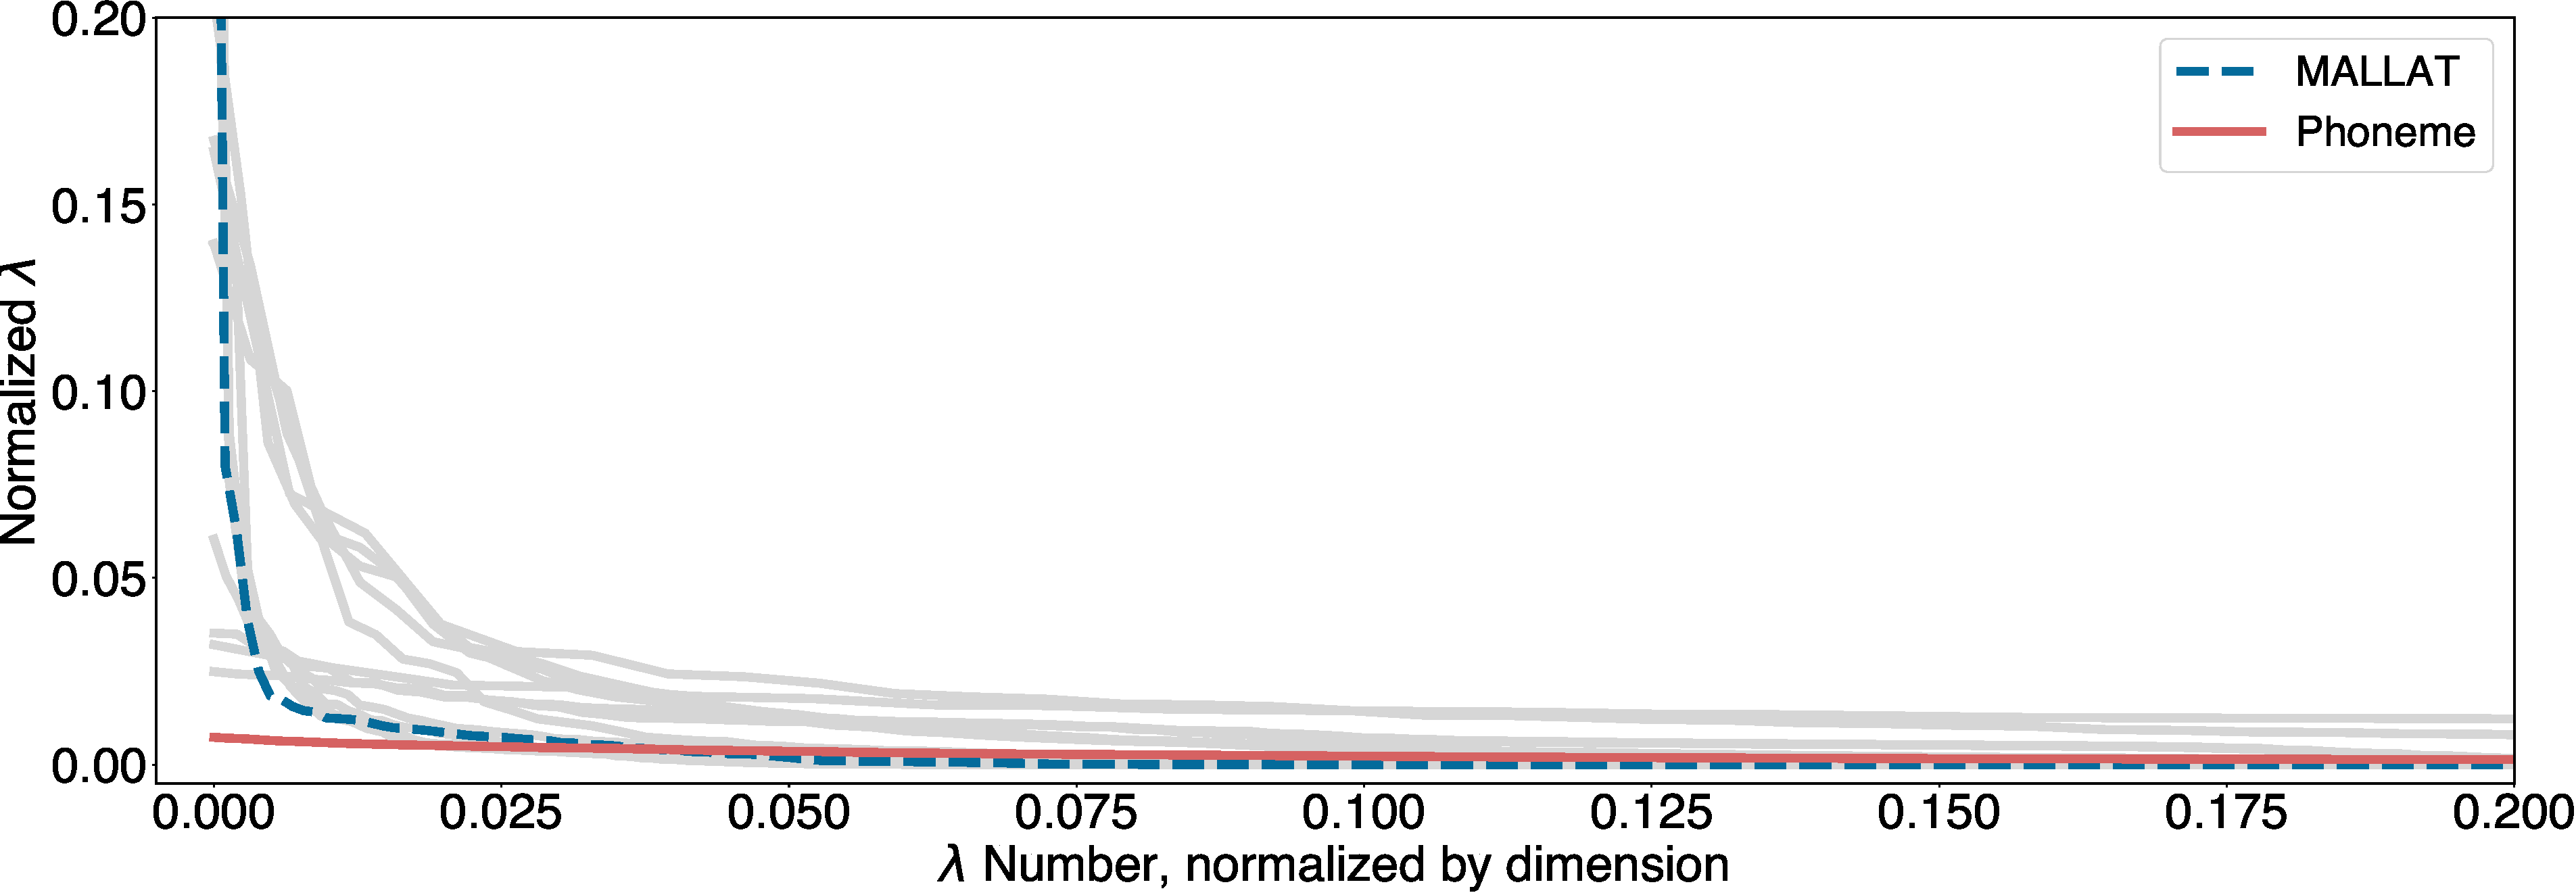
\includegraphics[width=\linewidth]{figs/spectrum-rev.pdf}
%\caption[]{Spectrum of UCR data highlighting MALLAT (performs well) and Phoneme (performs poorly).}
%\label{fig:spectrum}
%\end{figure}


\red{
\subsection{Streaming Execution}
\label{subsec:streaming}
%DROP can be extended to repeated-query scenarios that occur in a streaming context, where users wish to query incoming data against historical data.
%For instance, time series for similarity search are often generated as via systems that continuously monitor and obtain data from processes over a large span of time.
%Users wish to process this data as it arrives to identify anomalous or interesting behavior.
% (e.g., to identify repetitive seismic activity/earthquakes~\cite{quakes}).

Given a stationary input distribution, users can extract fixed-length sliding windows from the source and apply DROP's transformation over these segments as they arrive. 
Should the data distribution not be stationary over time, DROP can be be periodically retrained in one of two ways. 
First, DROP can use of the wide body of work in changepoint or feature drift detection~\cite{cp1, cp2} to determine when to retrain. 
Alternatively, DROP can maintain a reservoir sample of incoming data~\cite{reservoir}, tuned to the specific application, and retrain if the metric of interest no longer satisfies user-specified constraints. 
Due to DROP's default termination condition, cost-based optimization must be disabled until the metric constraint is achieved to prevent early termination.

}




%
\begin{comment}
\begin{figure}
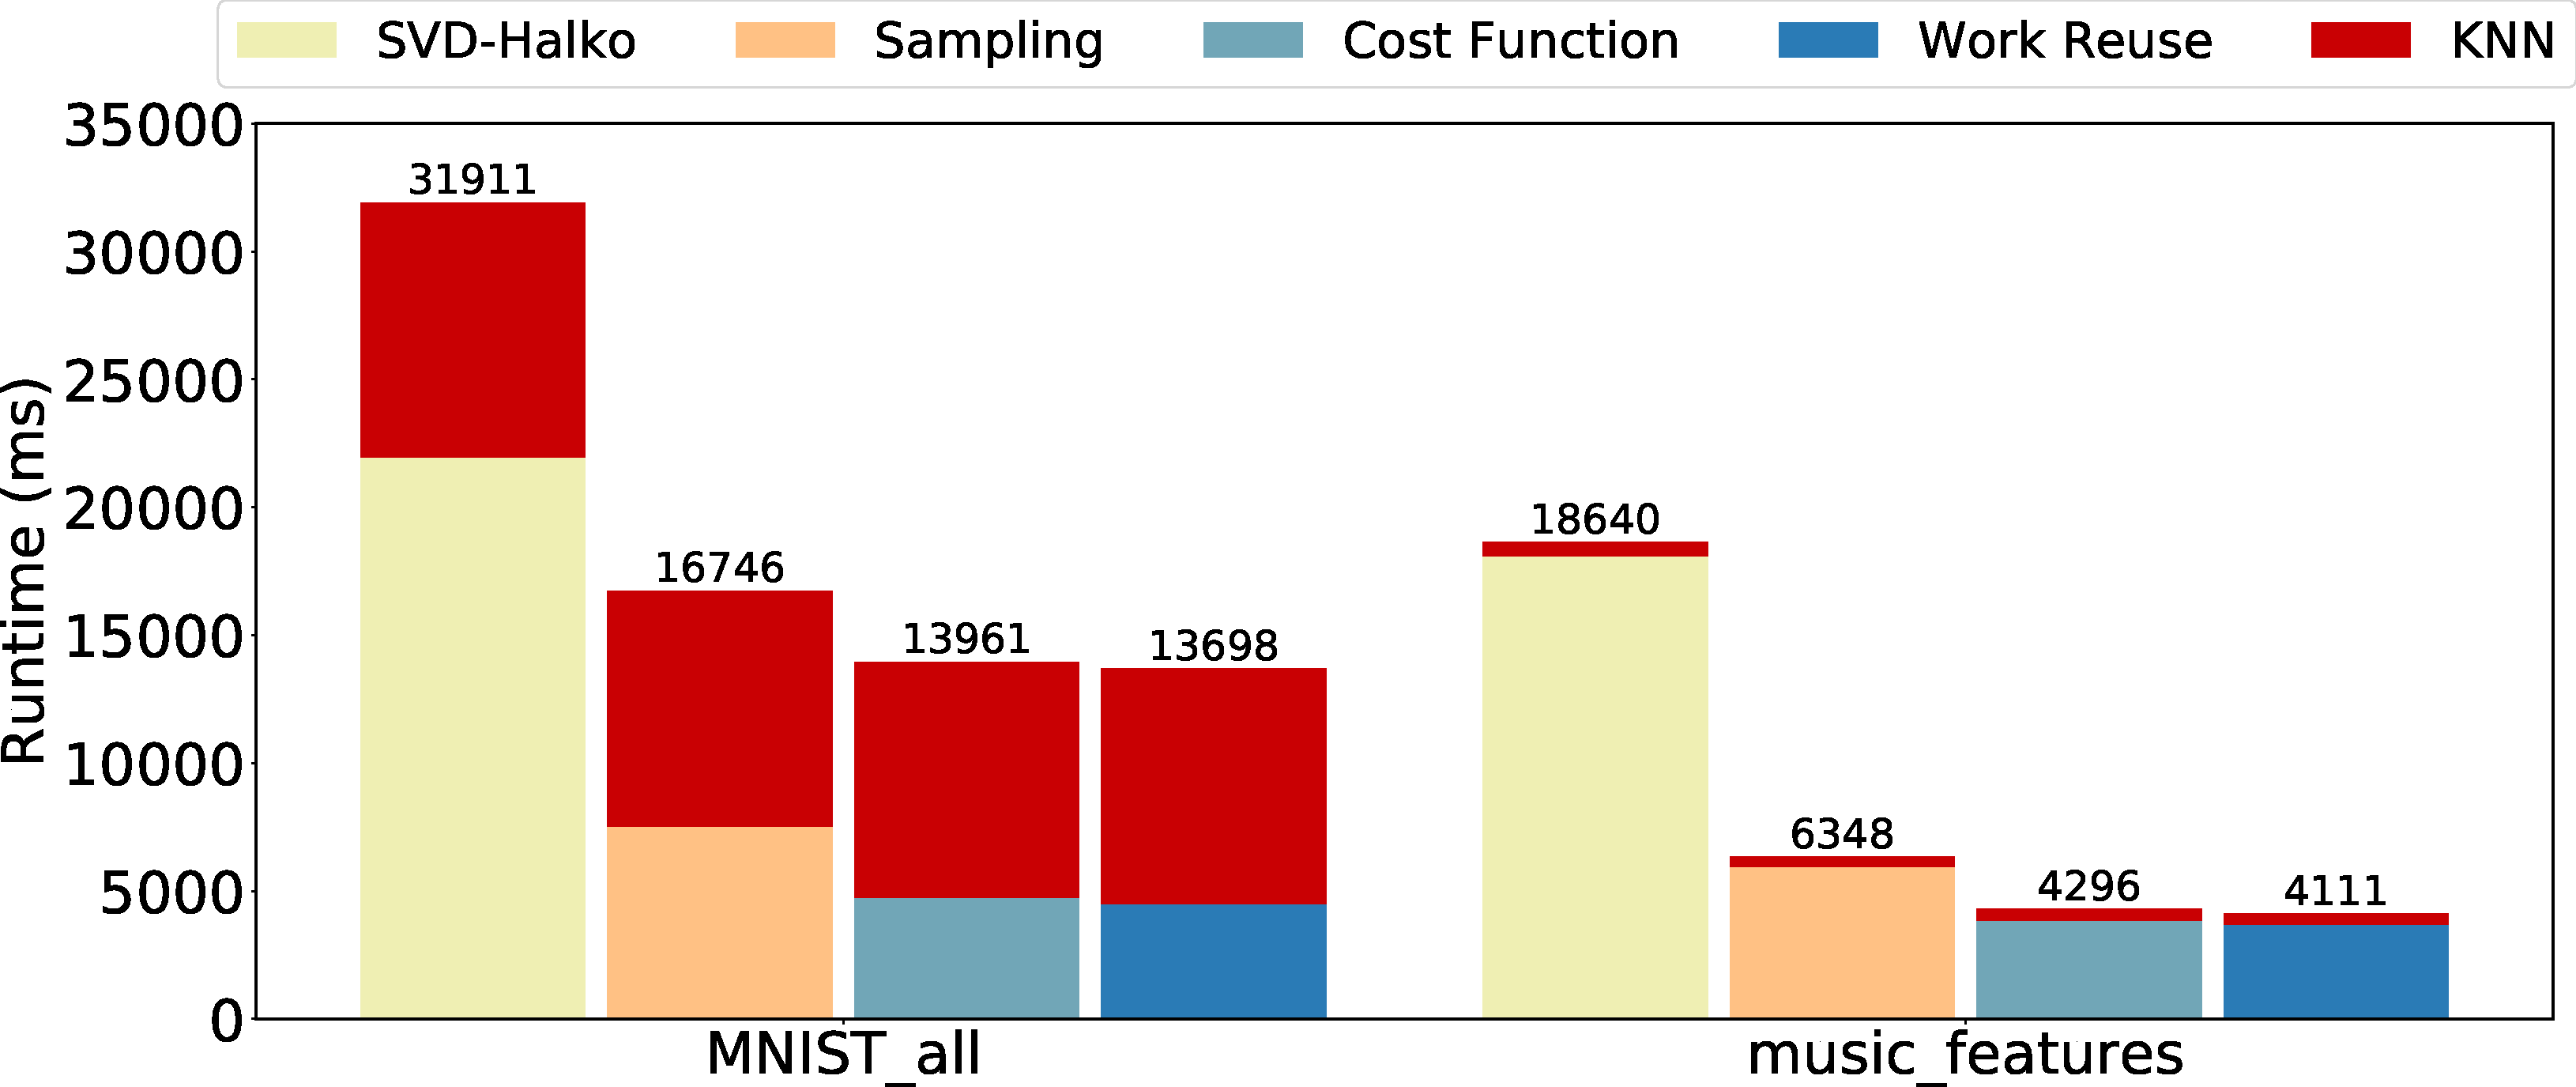
\includegraphics[width=\linewidth]{figs/beyond_tss_lesion.pdf}
\caption[]{End-to-End runtime lesion study of the entire MNIST dataset and the FMA featurized music dataset. Each of DROP's contributions provides a runtime improvement.}
\label{fig:beyond_lesion}
\end{figure}
\end{comment}



\section{Conclusion}
\label{sec:conclusion}

Advanced data analytics techniques must scale to rising data volumes. 
DR techniques offer a powerful toolkit when processing these datasets, with PCA frequently outperforming popular techniques in exchange for high computational cost. 
In response, we propose DROP, a new dimensionality reduction optimizer. 
DROP combines progressive sampling, progress estimation, and online aggregation to identify high quality low dimensional bases via PCA without processing the entire dataset by balancing the runtime of downstream tasks and achieved dimensionality. 
Thus, DROP provides a first step in bridging the gap between quality and efficiency in end-to-end DR for downstream \red{analytics}. 

%We revisit canonical operators for time series dimensionality reduction and the measurement study of~\cite{keogh-study}, and show that PCA is more effective than popular alternatives in the data mining literature often by a margin of over $2\times$ on average on gold-standard time series benchmark data sets with respect to output data dimension. More surprisingly, we empirically demonstrate that a small number of samples are sufficient to accurately characterize directions of maximum variance and obtain a high-quality low-dimensional transformation.




\bibliographystyle{ACM-Reference-Format}
\bibliography{drop}
%\appendix
\section*{APPENDIX}

\section{Augmented Results}


In this section, we provide additional information to augment results provided in our time series case study. 
Table~\ref{tab:sample} displays the proportion of data required to attain a given $TLB$ when using a PCA transformation where output dimension is equal to input dimension. Table~\ref{tab:kneeded} illustrates the output dimension required for each algorithm (PAA, FFT, and PCA) to attain a target $TLB$. 
Table~\ref{tab:runtime-comparison} illustrates the different running times of each algorithm (PAA, FFT, and PCA), and how sampling using the proportion from Table~\ref{tab:sample} for $TLB=0.99$ can help bridge the time gap between SVD and other techniques. 
%Finally, we provide all of the remaining lesion studies for the UCR dataset.


\begin{table}[]
\centering
\caption{Normalized lower dimension for target $TLB$ across DR techniques. PCA admits lower dimension for most UCR time series datasets.}
\label{tab:kneeded}
\scriptsize
\begin{tabular}{|l|r|r|r|r|r|r|}
\hline
                                  & \multicolumn{3}{c|}{\textbf{TLB:0.75}}     & \multicolumn{3}{c|}{\textbf{TLB:0.99}}     \\ \hline
\textbf{Dataset (dimension)} & \textit{PAA} & \textit{FFT} & \textit{PCA} & \textit{PAA} & \textit{FFT} & \textit{PCA} \\ \hline
ElectricDevices (96)              & 0.126        & 0.094        & 0.032        & 0.594        & 0.212        & 0.164        \\ \hline
FordA (500)                       & 0.138        & 0.098        & 0.038        & 0.636        & 0.214        & 0.17         \\ \hline
FordB (500)                       & 0.018        & 0.029        & 0.009        & 0.290        & 0.177        & 0.035        \\ \hline
MALLAT (1024)                     & 0.084        & 0.068        & 0.057        & 0.898        & 0.837        & 0.522        \\ \hline
Phoneme (1024)                    & 0.004        & 0.026        & 0.001        & 0.049        & 0.035        & 0.034        \\ \hline
StarLightCurves (1024)            & 0.015        & 0.028        & 0.019        & 0.037        & 0.086        & 0.062        \\ \hline
UWGLAll (945)                     & 0.078        & 0.065        & 0.026        & 0.822        & 0.736        & 0.322        \\ \hline
wafer (152)                       & 0.014        & 0.030        & 0.007        & 0.103        & 0.049        & 0.037        \\ \hline
yoga (426)                        & 0.375        & 0.375        & 0.281        & 0.812        & 0.822        & 0.770        \\ \hline

\end{tabular}
\end{table}



\begin{table}[]
\centering
\caption{Runtime (in ms) of 3 DR techniques. PCA is slowest, and can be over $56\times$ slower than PAA. Running SVD over a sample can bridge this gap.}
\label{tab:runtime-comparison}
\scriptsize
\begin{tabular}{|l|c|c|c|c|}
\hline
\textbf{Dataset}        & \textbf{PAA ($\times$SVD)} & \textbf{FFT} & \textbf{SVD} & \textbf{Sampling} \\ \hline
ElectricDevices         & 3 (9.8$\times$)            & 18           & 33           & 6                 \\ \hline
FordA                   & 7 (19$\times$)             & 38           & 137          & 8                 \\ \hline
FordB                   & 7 (18$\times$)             & 32           & 121          & 7                 \\ \hline
MALLAT                  & 7 (37.6$\times$)           & 35           & 278          & 5                 \\ \hline
Phoneme                 & 5 (56.2$\times$)           & 29           & 281          & 164               \\ \hline
StarLightCurves         & 19 (24.1$\times$)          & 120          & 457          & 5                 \\ \hline
UWGLAll & 7 (43.5$\times$)           & 56           & 287          & 8                 \\ \hline
Wafer                   & 4 (6.1$\times$)            & 13           & 22           & 5                 \\ \hline
Yoga                    & 4 (21.2$\times$)           & 29           & 81           & 8                 \\ \hline
\end{tabular}
\end{table}



\begin{table}[]
\centering
\scriptsize
\caption{A small proportion of data is needed to obtain a $TLB$-preserving transform with full PCA (output = input dimension).}

\begin{tabular}{|l|r|r|r|}
\hline
                               & \multicolumn{3}{c|}{\textit{\textbf{TLB}}}    \\ \hline
\textbf{Dataset (number of datapoints)}               & \textbf{0.75} & \textbf{0.90} & \textbf{0.99} \\ \hline
ElectricDevices (16637)               & 0.0026        & 0.0043        & 0.0088        \\ \hline
FordA   (4921)                       & 0.0054        & 0.0114        & 0.0198        \\ \hline
FordB   (4446)                       & 0.008         & 0.0146        & 0.0248        \\ \hline
MALLAT  (2400)                       & 0.0031        & 0.009         & 0.0197        \\ \hline
Phoneme   (2110)                     & 0.0547        & 0.1346        & 0.3875        \\ \hline
StarLightCurves (9236)               & 0.001         & 0.0011        & 0.0039        \\ \hline
UWGLAll  (4478)       & 0.0025        & 0.0056        & 0.024         \\ \hline
wafer  (7164)                        & 0.001         & 0.0032        & 0.0097        \\ \hline
yoga  (3300)                         & 0.0017        & 0.0028        & 0.0096        \\ \hline
\end{tabular}
\label{tab:sample}
\end{table}






\begin{comment}
\begin{table}[b]
\centering
\scriptsize
\caption{End-to-End runtime comparison of DROP and baseline techniques with k-NN retrieval task, in ms}
\label{tab:eefull}
\begin{tabular}{|l|c|c|c|c|c|}
\hline
\textbf{Dataset}       & \textbf{No DR} & \textbf{SVD} & \textbf{SVD-Halko} & \textbf{Oracle} & \textbf{DROP} \\ \hline
ChlorineConcentration  & 458   & 4054  & 424   & 207   & 178   \\ \hline
CinC                   & 1809  & 3068  & 5738  & 884   & 894   \\ \hline
ECG5000                & 1855  & 5689  & 561   & 362   & 482   \\ \hline
ElectricDevices        & 38222 & 83302 & 28433 & 27260 & 30701 \\ \hline
FordA                  & 21906 & 10546 & 5300  & 4270  & 4286  \\ \hline
FordB                  & 18271 & 8984  & 4917  & 3773  & 3792  \\ \hline
HandOutlines           & 5160  & 5620  & 9479  & 2832  & 2678  \\ \hline
InlineSkate            & 579   & 1420  & 2081  & 548   & 704   \\ \hline
InsectWingbeatSound    & 805   & 977   & 425   & 200   & 212   \\ \hline
MALLAT                 & 2593  & 2895  & 3870  & 643   & 450   \\ \hline
NonInvasiveFatalECG    & 5157  & 5229  & 3235  & 944   & 1043  \\ \hline
Phoneme                & 8490  & 6710  & 7687  & 7534  & 10446 \\ \hline
StarLightCurves        & 32024 & 35129 & 11429 & 1079  & 1238  \\ \hline
Two                    & 5728  & 8916  & 2849  & 2860  & 3335  \\ \hline
UWaveGestureLibraryAll & 25825 & 8147  & 5509  & 1298  & 1355  \\ \hline
uWaveGestureLibrary    & 4734  & 5669  & 1067  & 402   & 310   \\ \hline
wafer                  & 1536  & 12911 & 749   & 403   & 403   \\ \hline
yoga                   & 1199  & 2943  & 1029  & 174   & 153   \\ \hline
\end{tabular}
\end{table}


\begin{table}[b]
\centering
\scriptsize
\caption{Raw accuracy in k-NN retrieval task}
\label{tab:knn}
\begin{tabular}{|l|c|c|c|c|}
\hline
\textbf{Dataset}   & \textbf{SVD} & \textbf{SVD-Halko} & \textbf{Oracle} & \textbf{DROP} \\ \hline
ChlorineConcentration  & 0.893        & 0.886              & 0.906           & 0.903         \\ \hline
CinC                   & 0.894        & 0.892              & 0.899           & 0.929         \\ \hline
ECG5000                & 0.855        & 0.855              & 0.856           & 0.874         \\ \hline
ElectricDevices        & 0.877        & 0.875              & 0.866           & 0.888         \\ \hline
FordA                  & 0.892        & 0.878              & 0.884           & 0.9           \\ \hline
FordB                  & 0.875        & 0.875              & 0.871           & 0.874         \\ \hline
HandOutlines           & 0.908        & 0.901              & 0.907           & 0.92          \\ \hline
InlineSkate            & 0.832        & 0.818              & 0.803           & 0.805         \\ \hline
InsectWingbeatSound    & 0.815        & 0.815              & 0.811           & 0.848         \\ \hline
MALLAT                 & 0.83         & 0.83               & 0.876           & 0.892         \\ \hline
NonInvasiveFatalECG    & 0.82         & 0.822              & 0.836           & 0.827         \\ \hline
Phoneme                & 0.848        & 0.852              & 0.68            & 0.678         \\ \hline
StarLightCurves        & 0.615        & 0.648              & 0.653           & 0.651         \\ \hline
Two                    & 0.899        & 0.903              & 0.901           & 0.902         \\ \hline
UWaveGestureLibraryAll & 0.846        & 0.853              & 0.856           & 0.883         \\ \hline
uWaveGestureLibrary    & 0.797        & 0.797              & 0.808           & 0.838         \\ \hline
wafer                  & 0.808        & 0.818              & 0.833           & 0.888         \\ \hline
yoga                   & 0.791        & 0.791              & 0.797           & 0.818         \\ \hline
\end{tabular}
\end{table}


\end{comment}


\begin{comment}
\begin{table*}[]
\centering
\scriptsize
\caption{Output dimension required for target $TLB$ across dimensionality reduction technique (right 9 data columns), and proportion of data required to obtain a $TLB$-preserving PCA transformation with output dimension = input dimension (final 3 columns)}
\label{tab:bigtab}
\begin{tabular}{| c ||ccc|ccc|ccc||cc||ccc|}
\hline

 & \multicolumn{3}{c|}{\textbf{TLB: 0.75}} & \multicolumn{3}{c|}{\textbf{TLB: 0.90}} & \multicolumn{3}{c||}{\textbf{TLB: 0.99}} &  &  & \multicolumn{3}{c|}{\textbf{TLB}}  \\

\textbf{Dataset} & \textit{PAA }     & \textit{FFT}     & \textit{PCA}     & \textit{PAA}      & \textit{FFT}      & \textit{PCA}     & \textit{PAA}      & \textit{FFT}     &\textit{PCA}     &  &  & \textit{0.75}   & \textit{0.90 }  & \textit{0.99}   \\
\hline
50words                        & 9        & 9        & 7       & 18       & 14       & 10      & 62       & 28       & 25      &  &  & 0.0106 & 0.0185 & 0.0391 \\
Adiac                          & 7        & 8        & 4       & 15       & 13       & 6       & 69       & 34       & 20      &  &  & 0.0077 & 0.0145 & 0.0484 \\
ArrowHead                      & 9        & 9        & 4       & 16       & 13       & 8       & 73       & 33       & 26      &  &  & 0.0285 & 0.0626 & 0.2907 \\
Beef                           & 7        & 15       & 2       & 20       & 18       & 3       & 89       & 48       & 7       &  &  & 0.0494 & 0.0898 & 0.19   \\
BeetleFly                      & 16       & 16       & 6       & 28       & 21       & 12      & 99       & 34       & 22      &  &  & 0.3073 & 0.4449 & 0.7979 \\
BirdChicken                    & 8        & 14       & 3       & 14       & 17       & 6       & 48       & 20       & 15      &  &  & 0.156  & 0.2357 & 0.5437 \\
Car                            & 7        & 16       & 2       & 15       & 19       & 6       & 70       & 37       & 24      &  &  & 0.0428 & 0.0979 & 0.3719 \\
CBF                            & 15       & 13       & 7       & 61       & 57       & 45      & 114      & 114      & 107     &  &  & 0.0273 & 0.0775 & 0.1407 \\
ChlorineConcentration          & 46       & 34       & 2       & 93       & 81       & 5       & 153      & 153      & 30      &  &  & 0.001  & 0.0029 & 0.014  \\
CinC                           & 29       & 44       & 26      & 58       & 53       & 40      & 241      & 107      & 48      &  &  & 0.007  & 0.0157 & 0.0391 \\
Coffee                         & 14       & 17       & 3       & 46       & 37       & 6       & 225      & 158      & 38      &  &  & 0.1224 & 0.2715 & 0.8632 \\
Computers                      & 21       & 24       & 16      & 94       & 66       & 44      & 636      & 614      & 192     &  &  & 0.0596 & 0.1889 & 0.6818 \\
Cricket                        & 14       & 14       & 9       & 47       & 35       & 21      & 248      & 202      & 113     &  &  & 0.0198 & 0.0574 & 0.2488 \\
DiatomSizeReduction            & 7        & 11       & 7       & 11       & 13       & 10      & 87       & 55       & 21      &  &  & 0.015  & 0.0282 & 0.176  \\
DistalPhalanxOutlineAgeGroup   & 12       & 12       & 2       & 27       & 17       & 6       & 66       & 60       & 36      &  &  & 0.0094 & 0.0241 & 0.0987 \\
DistalPhalanxOutlineCorrect    & 12       & 12       & 2       & 26       & 16       & 7       & 66       & 57       & 32      &  &  & 0.006  & 0.0168 & 0.0642 \\
DistalPhalanxTW                & 12       & 12       & 2       & 27       & 16       & 6       & 66       & 60       & 34      &  &  & 0.0097 & 0.0236 & 0.098  \\
Earthquakes                    & 276      & 269      & 103     & 410      & 400      & 190     & 491      & 490      & 340     &  &  & 0.3733 & 0.6052 & 0.8988 \\
ECG200                         & 8        & 7        & 3       & 29       & 22       & 6       & 72       & 56       & 41      &  &  & 0.0288 & 0.0942 & 0.3287 \\
ECG5000                        & 14       & 14       & 3       & 30       & 24       & 7       & 115      & 88       & 31      &  &  & 0.001  & 0.0025 & 0.0132 \\
ECGFiveDays                    & 31       & 28       & 2       & 53       & 40       & 5       & 111      & 65       & 13      &  &  & 0.0073 & 0.0114 & 0.0275 \\
ElectricDevices                & 36       & 36       & 27      & 62       & 57       & 49      & 78       & 79       & 74      &  &  & 0.0026 & 0.0043 & 0.0088 \\
FaceAll                        & 28       & 24       & 8       & 50       & 35       & 20      & 110      & 81       & 48      &  &  & 0.0078 & 0.0171 & 0.0355 \\
FaceFour                       & 36       & 31       & 5       & 67       & 43       & 12      & 277      & 228      & 61      &  &  & 0.1143 & 0.2727 & 0.7708 \\
FacesUCR                       & 28       & 24       & 9       & 48       & 34       & 22      & 109      & 53       & 49      &  &  & 0.0077 & 0.0169 & 0.0355 \\
FISH                           & 10       & 15       & 5       & 20       & 18       & 11      & 91       & 37       & 28      &  &  & 0.0181 & 0.0433 & 0.1587 \\
FordA                          & 63       & 47       & 16      & 98       & 61       & 35      & 297      & 106      & 82      &  &  & 0.0054 & 0.0114 & 0.0198 \\
FordB                          & 69       & 49       & 19      & 102      & 65       & 39      & 318      & 107      & 85      &  &  & 0.008  & 0.0146 & 0.0248 \\
Gun                            & 5        & 6        & 3       & 11       & 9        & 5       & 56       & 24       & 14      &  &  & 0.0282 & 0.0477 & 0.134  \\
Ham                            & 34       & 32       & 7       & 73       & 58       & 18      & 261      & 114      & 61      &  &  & 0.0811 & 0.1558 & 0.4486 \\
HandOutlines                   & 11       & 70       & 10      & 25       & 83       & 32      & 93       & 91       & 46      &  &  & 0.0045 & 0.0091 & 0.0372 \\
Haptics                        & 10       & 29       & 6       & 19       & 35       & 14      & 173      & 81       & 32      &  &  & 0.017  & 0.0394 & 0.1234 \\
Herring                        & 10       & 15       & 3       & 25       & 18       & 8       & 111      & 63       & 39      &  &  & 0.0599 & 0.1447 & 0.4878 \\
InlineSkate                    & 7        & 49       & 7       & 15       & 58       & 17      & 55       & 63       & 22      &  &  & 0.0085 & 0.0162 & 0.0388 \\
InsectWingbeatSound            & 15       & 14       & 7       & 28       & 22       & 13      & 100      & 42       & 33      &  &  & 0.0048 & 0.0119 & 0.0255 \\
ItalyPowerDemand               & 6        & 6        & 2       & 11       & 10       & 5       & 19       & 17       & 15      &  &  & 0.0068 & 0.01   & 0.0198 \\
LargeKitchenAppliances         & 59       & 49       & 36      & 165      & 125      & 89      & 624      & 545      & 284     &  &  & 0.0987 & 0.2373 & 0.6068 \\
Lighting2                      & 41       & 34       & 9       & 152      & 149      & 28      & 557      & 490      & 82      &  &  & 0.186  & 0.4505 & 0.9132 \\
Lighting7                      & 31       & 27       & 9       & 126      & 118      & 26      & 280      & 269      & 81      &  &  & 0.1439 & 0.3534 & 0.9022 \\
MALLAT                         & 19       & 30       & 10      & 46       & 36       & 26      & 297      & 182      & 36      &  &  & 0.0031 & 0.009  & 0.0197 \\
Meat                           & 13       & 14       & 2       & 32       & 24       & 4       & 218      & 213      & 23      &  &  & 0.0398 & 0.0528 & 0.3494 \\
MedicalImages                  & 12       & 10       & 3       & 20       & 17       & 7       & 66       & 34       & 17      &  &  & 0.007  & 0.0103 & 0.0256 \\
MiddlePhalanxOutlineAgeGroup   & 12       & 12       & 2       & 27       & 16       & 4       & 66       & 60       & 31      &  &  & 0.0096 & 0.0191 & 0.0939 \\
MiddlePhalanxOutlineCorrect    & 12       & 12       & 2       & 27       & 16       & 5       & 66       & 58       & 30      &  &  & 0.0065 & 0.0127 & 0.0548 \\
MiddlePhalanxTW                & 12       & 12       & 2       & 27       & 16       & 5       & 66       & 60       & 32      &  &  & 0.0089 & 0.0206 & 0.0916 \\
MoteStrain                     & 12       & 11       & 7       & 39       & 37       & 26      & 76       & 75       & 63      &  &  & 0.0148 & 0.0323 & 0.0838 \\
NonInvasiveFatalECG            & 16       & 22       & 3       & 42       & 31       & 18      & 201      & 121      & 82      &  &  & 0.0021 & 0.0043 & 0.0375 \\
OliveOil                       & 33       & 25       & 2       & 61       & 51       & 5       & 375      & 213      & 23      &  &  & 0.0936 & 0.1727 & 0.6366 \\
OSULeaf                        & 11       & 13       & 9       & 20       & 16       & 14      & 73       & 30       & 29      &  &  & 0.0258 & 0.0435 & 0.1104 \\
PhalangesOutlinesCorrect       & 11       & 12       & 2       & 26       & 16       & 5       & 65       & 56       & 28      &  &  & 0.0023 & 0.0046 & 0.0187 \\
Phoneme                        & 87       & 70       & 59      & 268      & 201      & 160     & 920      & 858      & 535     &  &  & 0.0547 & 0.1346 & 0.3875 \\
Plane                          & 12       & 11       & 3       & 22       & 14       & 6       & 76       & 39       & 21      &  &  & 0.0285 & 0.0683 & 0.2068 \\
ProximalPhalanxOutlineAgeGroup & 12       & 12       & 2       & 26       & 18       & 4       & 65       & 58       & 28      &  &  & 0.0068 & 0.0171 & 0.0825 \\
ProximalPhalanxOutlineCorrect  & 12       & 12       & 2       & 27       & 18       & 5       & 66       & 58       & 28      &  &  & 0.0046 & 0.0134 & 0.0512 \\
ProximalPhalanxTW              & 12       & 12       & 2       & 26       & 18       & 5       & 65       & 59       & 28      &  &  & 0.0052 & 0.0153 & 0.0831 \\
RefrigerationDevices           & 94       & 76       & 60      & 222      & 154      & 121     & 645      & 586      & 316     &  &  & 0.1414 & 0.2777 & 0.6696 \\
ScreenType                     & 18       & 24       & 20      & 70       & 55       & 40      & 614      & 614      & 207     &  &  & 0.0324 & 0.1087 & 0.5341 \\
ShapeletSim                    & 275      & 272      & 62      & 410      & 402      & 111     & 491      & 490      & 180     &  &  & 0.497  & 0.7498 & 0.969  \\
ShapesAll                      & 7        & 14       & 7       & 14       & 17       & 14      & 49       & 25       & 20      &  &  & 0.0048 & 0.0137 & 0.0278 \\
SmallKitchenAppliances         & 259      & 235      & 104     & 497      & 423      & 204     & 698      & 678      & 398     &  &  & 0.2489 & 0.422  & 0.7194 \\
SonyAIBORobotSurface           & 15       & 14       & 5       & 28       & 21       & 13      & 56       & 43       & 38      &  &  & 0.0211 & 0.0442 & 0.0969 \\
SonyAIBORobotSurfaceII         & 18       & 18       & 6       & 30       & 24       & 13      & 57       & 45       & 39      &  &  & 0.0143 & 0.0272 & 0.0708 \\
StarLightCurves                & 5        & 27       & 2       & 14       & 33       & 21      & 51       & 36       & 35      &  &  & 0.001  & 0.0011 & 0.0039 \\
Strawberry                     & 10       & 11       & 2       & 24       & 21       & 6       & 98       & 41       & 13      &  &  & 0.005  & 0.0086 & 0.0225 \\
SwedishLeaf                    & 9        & 9        & 5       & 19       & 14       & 10      & 71       & 37       & 32      &  &  & 0.0083 & 0.0178 & 0.0727 \\
Symbols                        & 7        & 11       & 6       & 12       & 13       & 11      & 46       & 26       & 14      &  &  & 0.0071 & 0.0096 & 0.0246 \\
synthetic                      & 14       & 14       & 7       & 37       & 38       & 28      & 58       & 59       & 54      &  &  & 0.0281 & 0.0642 & 0.0964 \\
ToeSegmentation1               & 12       & 10       & 8       & 24       & 19       & 16      & 116      & 49       & 43      &  &  & 0.0548 & 0.0992 & 0.2988 \\
ToeSegmentation2               & 10       & 13       & 6       & 21       & 20       & 13      & 101      & 49       & 34      &  &  & 0.0718 & 0.144  & 0.3784 \\
Trace                          & 6        & 9        & 2       & 18       & 17       & 7       & 120      & 69       & 31      &  &  & 0.0222 & 0.0555 & 0.3752 \\
TwoLeadECG                     & 12       & 9        & 2       & 25       & 19       & 4       & 70       & 51       & 14      &  &  & 0.0045 & 0.0081 & 0.0259 \\
Two                            & 13       & 11       & 7       & 34       & 24       & 20      & 108      & 102      & 98      &  &  & 0.0038 & 0.0097 & 0.0259 \\
UWaveGestureLibraryAll         & 15       & 27       & 18      & 35       & 32       & 28      & 151      & 82       & 59      &  &  & 0.0025 & 0.0056 & 0.024  \\
uWaveGestureLibrary            & 4        & 10       & 5       & 10       & 11       & 10      & 43       & 27       & 20      &  &  & 0.0017 & 0.0024 & 0.0081 \\
wafer                          & 12       & 10       & 4       & 37       & 29       & 11      & 125      & 112      & 49      &  &  & 0.001  & 0.0032 & 0.0097 \\
Wine                           & 10       & 9        & 2       & 27       & 20       & 3       & 104      & 58       & 9       &  &  & 0.031  & 0.0477 & 0.1745 \\
WordsSynonyms                  & 9        & 9        & 7       & 17       & 14       & 10      & 62       & 31       & 25      &  &  & 0.0094 & 0.0196 & 0.0389 \\
Worms                          & 9        & 26       & 8       & 26       & 30       & 17      & 123      & 62       & 41      &  &  & 0.0661 & 0.109  & 0.3177 \\
WormsTwoClass                  & 10       & 26       & 8       & 25       & 30       & 17      & 124      & 61       & 42      &  &  & 0.0575 & 0.1193 & 0.3289 \\
yoga                           & 6        & 13       & 3       & 11       & 15       & 11      & 44       & 21       & 16      &  &  & 0.0017 & 0.0028 & 0.0096 \\
\hline
\end{tabular}
\end{table*}
\end{comment}


\begin{comment}
\begin{table}[H]
\centering
\scriptsize
\caption{Proportion of data required to obtain a $TLB$-preserving transformation with full PCA (i.e., output dimension = input dimension)}

\begin{tabular}{|l|c|c|c|}
\hline
                               & \multicolumn{3}{c|}{\textit{\textbf{TLB}}}    \\ \hline
\textbf{Dataset}               & \textbf{0.75} & \textbf{0.90} & \textbf{0.99} \\ \hline
50words                        & 0.0106        & 0.0185        & 0.0391        \\ \hline
Adiac                          & 0.0077        & 0.0145        & 0.0484        \\ \hline
ArrowHead                      & 0.0285        & 0.0626        & 0.2907        \\ \hline
Beef                           & 0.0494        & 0.0898        & 0.19          \\ \hline
BeetleFly                      & 0.3073        & 0.4449        & 0.7979        \\ \hline
BirdChicken                    & 0.156         & 0.2357        & 0.5437        \\ \hline
Car                            & 0.0428        & 0.0979        & 0.3719        \\ \hline
CBF                            & 0.0273        & 0.0775        & 0.1407        \\ \hline
ChlorineConcentration          & 0.001         & 0.0029        & 0.014         \\ \hline
CinC                           & 0.007         & 0.0157        & 0.0391        \\ \hline
Coffee                         & 0.1224        & 0.2715        & 0.8632        \\ \hline
Computers                      & 0.0596        & 0.1889        & 0.6818        \\ \hline
Cricket                        & 0.0198        & 0.0574        & 0.2488        \\ \hline
DiatomSizeReduction            & 0.015         & 0.0282        & 0.176         \\ \hline
DistalPhalanxOutlineAgeGroup   & 0.0094        & 0.0241        & 0.0987        \\ \hline
DistalPhalanxOutlineCorrect    & 0.006         & 0.0168        & 0.0642        \\ \hline
DistalPhalanxTW                & 0.0097        & 0.0236        & 0.098         \\ \hline
Earthquakes                    & 0.3733        & 0.6052        & 0.8988        \\ \hline
ECG200                         & 0.0288        & 0.0942        & 0.3287        \\ \hline
ECG5000                        & 0.001         & 0.0025        & 0.0132        \\ \hline
ECGFiveDays                    & 0.0073        & 0.0114        & 0.0275        \\ \hline
ElectricDevices                & 0.0026        & 0.0043        & 0.0088        \\ \hline
FaceAll                        & 0.0078        & 0.0171        & 0.0355        \\ \hline
FaceFour                       & 0.1143        & 0.2727        & 0.7708        \\ \hline
FacesUCR                       & 0.0077        & 0.0169        & 0.0355        \\ \hline
FISH                           & 0.0181        & 0.0433        & 0.1587        \\ \hline
FordA                          & 0.0054        & 0.0114        & 0.0198        \\ \hline
FordB                          & 0.008         & 0.0146        & 0.0248        \\ \hline
Gun                            & 0.0282        & 0.0477        & 0.134         \\ \hline
Ham                            & 0.0811        & 0.1558        & 0.4486        \\ \hline
HandOutlines                   & 0.0045        & 0.0091        & 0.0372        \\ \hline
Haptics                        & 0.017         & 0.0394        & 0.1234        \\ \hline
Herring                        & 0.0599        & 0.1447        & 0.4878        \\ \hline
InlineSkate                    & 0.0085        & 0.0162        & 0.0388        \\ \hline
InsectWingbeatSound            & 0.0048        & 0.0119        & 0.0255        \\ \hline
ItalyPowerDemand               & 0.0068        & 0.01          & 0.0198        \\ \hline
LargeKitchenAppliances         & 0.0987        & 0.2373        & 0.6068        \\ \hline
Lighting2                      & 0.186         & 0.4505        & 0.9132        \\ \hline
Lighting7                      & 0.1439        & 0.3534        & 0.9022        \\ \hline
MALLAT                         & 0.0031        & 0.009         & 0.0197        \\ \hline
Meat                           & 0.0398        & 0.0528        & 0.3494        \\ \hline
MedicalImages                  & 0.007         & 0.0103        & 0.0256        \\ \hline
MiddlePhalanxOutlineAgeGroup   & 0.0096        & 0.0191        & 0.0939        \\ \hline
MiddlePhalanxOutlineCorrect    & 0.0065        & 0.0127        & 0.0548        \\ \hline
MiddlePhalanxTW                & 0.0089        & 0.0206        & 0.0916        \\ \hline
MoteStrain                     & 0.0148        & 0.0323        & 0.0838        \\ \hline
NonInvasiveFatalECG            & 0.0021        & 0.0043        & 0.0375        \\ \hline
OliveOil                       & 0.0936        & 0.1727        & 0.6366        \\ \hline
OSULeaf                        & 0.0258        & 0.0435        & 0.1104        \\ \hline
PhalangesOutlinesCorrect       & 0.0023        & 0.0046        & 0.0187        \\ \hline
Phoneme                        & 0.0547        & 0.1346        & 0.3875        \\ \hline
Plane                          & 0.0285        & 0.0683        & 0.2068        \\ \hline
ProximalPhalanxOutlineAgeGroup & 0.0068        & 0.0171        & 0.0825        \\ \hline
ProximalPhalanxOutlineCorrect  & 0.0046        & 0.0134        & 0.0512        \\ \hline
ProximalPhalanxTW              & 0.0052        & 0.0153        & 0.0831        \\ \hline
RefrigerationDevices           & 0.1414        & 0.2777        & 0.6696        \\ \hline
ScreenType                     & 0.0324        & 0.1087        & 0.5341        \\ \hline
ShapeletSim                    & 0.497         & 0.7498        & 0.969         \\ \hline
ShapesAll                      & 0.0048        & 0.0137        & 0.0278        \\ \hline
SmallKitchenAppliances         & 0.2489        & 0.422         & 0.7194        \\ \hline
SonyAIBORobotSurface           & 0.0211        & 0.0442        & 0.0969        \\ \hline
SonyAIBORobotSurfaceII         & 0.0143        & 0.0272        & 0.0708        \\ \hline
StarLightCurves                & 0.001         & 0.0011        & 0.0039        \\ \hline
Strawberry                     & 0.005         & 0.0086        & 0.0225        \\ \hline
SwedishLeaf                    & 0.0083        & 0.0178        & 0.0727        \\ \hline
Symbols                        & 0.0071        & 0.0096        & 0.0246        \\ \hline
synthetic                      & 0.0281        & 0.0642        & 0.0964        \\ \hline
ToeSegmentation1               & 0.0548        & 0.0992        & 0.2988        \\ \hline
ToeSegmentation2               & 0.0718        & 0.144         & 0.3784        \\ \hline
Trace                          & 0.0222        & 0.0555        & 0.3752        \\ \hline
TwoLeadECG                     & 0.0045        & 0.0081        & 0.0259        \\ \hline
Two                            & 0.0038        & 0.0097        & 0.0259        \\ \hline
UWaveGestureLibraryAll         & 0.0025        & 0.0056        & 0.024         \\ \hline
uWaveGestureLibrary            & 0.0017        & 0.0024        & 0.0081        \\ \hline
wafer                          & 0.001         & 0.0032        & 0.0097        \\ \hline
Wine                           & 0.031         & 0.0477        & 0.1745        \\ \hline
WordsSynonyms                  & 0.0094        & 0.0196        & 0.0389        \\ \hline
Worms                          & 0.0661        & 0.109         & 0.3177        \\ \hline
WormsTwoClass                  & 0.0575        & 0.1193        & 0.3289        \\ \hline
yoga                           & 0.0017        & 0.0028        & 0.0096        \\ \hline
\end{tabular}
\label{tab:sampling}
\end{table}

\begin{table}[H]
\centering
\caption{Output dimension required for target $TLB$ across dimensionality reduction technique.}
\label{tab:baseK}
\scriptsize
\begin{tabular}{|l|c|c|c|c|c|c|c|c|c|l}
\cline{1-10}
\textbf{}                      & \multicolumn{3}{c|}{\textbf{TLB: 0.75}}    & \multicolumn{3}{c|}{\textbf{TLB: 0.90}}    & \multicolumn{3}{c|}{\textbf{TLB: 0.99}}    & \textbf{} \\ \cline{1-10}
\textbf{Dataset}               & \textit{PAA} & \textit{FFT} & \textit{PCA} & \textit{PAA} & \textit{FFT} & \textit{PCA} & \textit{PAA} & \textit{FFT} & \textit{PCA} & \textit{} \\ \cline{1-10}
50words                        & 9            & 9            & 7            & 18           & 14           & 10           & 62           & 28           & 25           &           \\ \cline{1-10}
Adiac                          & 7            & 8            & 4            & 15           & 13           & 6            & 69           & 34           & 20           &           \\ \cline{1-10}
ArrowHead                      & 9            & 9            & 4            & 16           & 13           & 8            & 73           & 33           & 26           &           \\ \cline{1-10}
Beef                           & 7            & 15           & 2            & 20           & 18           & 3            & 89           & 48           & 7            &           \\ \cline{1-10}
BeetleFly                      & 16           & 16           & 6            & 28           & 21           & 12           & 99           & 34           & 22           &           \\ \cline{1-10}
BirdChicken                    & 8            & 14           & 3            & 14           & 17           & 6            & 48           & 20           & 15           &           \\ \cline{1-10}
Car                            & 7            & 16           & 2            & 15           & 19           & 6            & 70           & 37           & 24           &           \\ \cline{1-10}
CBF                            & 15           & 13           & 7            & 61           & 57           & 45           & 114          & 114          & 107          &           \\ \cline{1-10}
ChlorineConcentration          & 46           & 34           & 2            & 93           & 81           & 5            & 153          & 153          & 30           &           \\ \cline{1-10}
CinC                           & 29           & 44           & 26           & 58           & 53           & 40           & 241          & 107          & 48           &           \\ \cline{1-10}
Coffee                         & 14           & 17           & 3            & 46           & 37           & 6            & 225          & 158          & 38           &           \\ \cline{1-10}
Computers                      & 21           & 24           & 16           & 94           & 66           & 44           & 636          & 614          & 192          &           \\ \cline{1-10}
Cricket                        & 14           & 14           & 9            & 47           & 35           & 21           & 248          & 202          & 113          &           \\ \cline{1-10}
DiatomSizeReduction            & 7            & 11           & 7            & 11           & 13           & 10           & 87           & 55           & 21           &           \\ \cline{1-10}
DPOAgeGroup   & 12           & 12           & 2            & 27           & 17           & 6            & 66           & 60           & 36           &           \\ \cline{1-10}
DPOCorrect    & 12           & 12           & 2            & 26           & 16           & 7            & 66           & 57           & 32           &           \\ \cline{1-10}
DistalPhalanxTW                & 12           & 12           & 2            & 27           & 16           & 6            & 66           & 60           & 34           &           \\ \cline{1-10}
Earthquakes                    & 276          & 269          & 103          & 410          & 400          & 190          & 491          & 490          & 340          &           \\ \cline{1-10}
ECG200                         & 8            & 7            & 3            & 29           & 22           & 6            & 72           & 56           & 41           &           \\ \cline{1-10}
ECG5000                        & 14           & 14           & 3            & 30           & 24           & 7            & 115          & 88           & 31           &           \\ \cline{1-10}
ECGFiveDays                    & 31           & 28           & 2            & 53           & 40           & 5            & 111          & 65           & 13           &           \\ \cline{1-10}
ElectricDevices                & 36           & 36           & 27           & 62           & 57           & 49           & 78           & 79           & 74           &           \\ \cline{1-10}
FaceAll                        & 28           & 24           & 8            & 50           & 35           & 20           & 110          & 81           & 48           &           \\ \cline{1-10}
FaceFour                       & 36           & 31           & 5            & 67           & 43           & 12           & 277          & 228          & 61           &           \\ \cline{1-10}
FacesUCR                       & 28           & 24           & 9            & 48           & 34           & 22           & 109          & 53           & 49           &           \\ \cline{1-10}
FISH                           & 10           & 15           & 5            & 20           & 18           & 11           & 91           & 37           & 28           &           \\ \cline{1-10}
FordA                          & 63           & 47           & 16           & 98           & 61           & 35           & 297          & 106          & 82           &           \\ \cline{1-10}
FordB                          & 69           & 49           & 19           & 102          & 65           & 39           & 318          & 107          & 85           &           \\ \cline{1-10}
Gun                            & 5            & 6            & 3            & 11           & 9            & 5            & 56           & 24           & 14           &           \\ \cline{1-10}
Ham                            & 34           & 32           & 7            & 73           & 58           & 18           & 261          & 114          & 61           &           \\ \cline{1-10}
HandOutlines                   & 11           & 70           & 10           & 25           & 83           & 32           & 93           & 91           & 46           &           \\ \cline{1-10}
Haptics                        & 10           & 29           & 6            & 19           & 35           & 14           & 173          & 81           & 32           &           \\ \cline{1-10}
Herring                        & 10           & 15           & 3            & 25           & 18           & 8            & 111          & 63           & 39           &           \\ \cline{1-10}
InlineSkate                    & 7            & 49           & 7            & 15           & 58           & 17           & 55           & 63           & 22           &           \\ \cline{1-10}
InsectWingbeatSound            & 15           & 14           & 7            & 28           & 22           & 13           & 100          & 42           & 33           &           \\ \cline{1-10}
ItalyPowerDemand               & 6            & 6            & 2            & 11           & 10           & 5            & 19           & 17           & 15           &           \\ \cline{1-10}
LargeKitchenAppliances         & 59           & 49           & 36           & 165          & 125          & 89           & 624          & 545          & 284          &           \\ \cline{1-10}
Lighting2                      & 41           & 34           & 9            & 152          & 149          & 28           & 557          & 490          & 82           &           \\ \cline{1-10}
Lighting7                      & 31           & 27           & 9            & 126          & 118          & 26           & 280          & 269          & 81           &           \\ \cline{1-10}
MALLAT                         & 19           & 30           & 10           & 46           & 36           & 26           & 297          & 182          & 36           &           \\ \cline{1-10}
Meat                           & 13           & 14           & 2            & 32           & 24           & 4            & 218          & 213          & 23           &           \\ \cline{1-10}
MedicalImages                  & 12           & 10           & 3            & 20           & 17           & 7            & 66           & 34           & 17           &           \\ \cline{1-10}
MPOAgeGroup   & 12           & 12           & 2            & 27           & 16           & 4            & 66           & 60           & 31           &           \\ \cline{1-10}
MPOCorrect    & 12           & 12           & 2            & 27           & 16           & 5            & 66           & 58           & 30           &           \\ \cline{1-10}
MiddlePhalanxTW                & 12           & 12           & 2            & 27           & 16           & 5            & 66           & 60           & 32           &           \\ \cline{1-10}
MoteStrain                     & 12           & 11           & 7            & 39           & 37           & 26           & 76           & 75           & 63           &           \\ \cline{1-10}
NonInvasiveFatalECG            & 16           & 22           & 3            & 42           & 31           & 18           & 201          & 121          & 82           &           \\ \cline{1-10}
OliveOil                       & 33           & 25           & 2            & 61           & 51           & 5            & 375          & 213          & 23           &           \\ \cline{1-10}
OSULeaf                        & 11           & 13           & 9            & 20           & 16           & 14           & 73           & 30           & 29           &           \\ \cline{1-10}
PhalangesOutlinesCorrect       & 11           & 12           & 2            & 26           & 16           & 5            & 65           & 56           & 28           &           \\ \cline{1-10}
Phoneme                        & 87           & 70           & 59           & 268          & 201          & 160          & 920          & 858          & 535          &           \\ \cline{1-10}
Plane                          & 12           & 11           & 3            & 22           & 14           & 6            & 76           & 39           & 21           &           \\ \cline{1-10}
PPOAgeGroup & 12           & 12           & 2            & 26           & 18           & 4            & 65           & 58           & 28           &           \\ \cline{1-10}
PPOCorrect  & 12           & 12           & 2            & 27           & 18           & 5            & 66           & 58           & 28           &           \\ \cline{1-10}
ProximalPhalanxTW              & 12           & 12           & 2            & 26           & 18           & 5            & 65           & 59           & 28           &           \\ \cline{1-10}
RefrigerationDevices           & 94           & 76           & 60           & 222          & 154          & 121          & 645          & 586          & 316          &           \\ \cline{1-10}
ScreenType                     & 18           & 24           & 20           & 70           & 55           & 40           & 614          & 614          & 207          &           \\ \cline{1-10}
ShapeletSim                    & 275          & 272          & 62           & 410          & 402          & 111          & 491          & 490          & 180          &           \\ \cline{1-10}
ShapesAll                      & 7            & 14           & 7            & 14           & 17           & 14           & 49           & 25           & 20           &           \\ \cline{1-10}
SmallKitchenAppliances         & 259          & 235          & 104          & 497          & 423          & 204          & 698          & 678          & 398          &           \\ \cline{1-10}
SonyAIBORobotSurface           & 15           & 14           & 5            & 28           & 21           & 13           & 56           & 43           & 38           &           \\ \cline{1-10}
SonyAIBORobotSurfaceII         & 18           & 18           & 6            & 30           & 24           & 13           & 57           & 45           & 39           &           \\ \cline{1-10}
StarLightCurves                & 5            & 27           & 2            & 14           & 33           & 21           & 51           & 36           & 35           &           \\ \cline{1-10}
Strawberry                     & 10           & 11           & 2            & 24           & 21           & 6            & 98           & 41           & 13           &           \\ \cline{1-10}
SwedishLeaf                    & 9            & 9            & 5            & 19           & 14           & 10           & 71           & 37           & 32           &           \\ \cline{1-10}
Symbols                        & 7            & 11           & 6            & 12           & 13           & 11           & 46           & 26           & 14           &           \\ \cline{1-10}
synthetic                      & 14           & 14           & 7            & 37           & 38           & 28           & 58           & 59           & 54           &           \\ \cline{1-10}
ToeSegmentation1               & 12           & 10           & 8            & 24           & 19           & 16           & 116          & 49           & 43           &           \\ \cline{1-10}
ToeSegmentation2               & 10           & 13           & 6            & 21           & 20           & 13           & 101          & 49           & 34           &           \\ \cline{1-10}
Trace                          & 6            & 9            & 2            & 18           & 17           & 7            & 120          & 69           & 31           &           \\ \cline{1-10}
TwoLeadECG                     & 12           & 9            & 2            & 25           & 19           & 4            & 70           & 51           & 14           &           \\ \cline{1-10}
Two                            & 13           & 11           & 7            & 34           & 24           & 20           & 108          & 102          & 98           &           \\ \cline{1-10}
UWGLAll         & 15           & 27           & 18           & 35           & 32           & 28           & 151          & 82           & 59           &           \\ \cline{1-10}
uWaveGestureLibrary            & 4            & 10           & 5            & 10           & 11           & 10           & 43           & 27           & 20           &           \\ \cline{1-10}
wafer                          & 12           & 10           & 4            & 37           & 29           & 11           & 125          & 112          & 49           &           \\ \cline{1-10}
Wine                           & 10           & 9            & 2            & 27           & 20           & 3            & 104          & 58           & 9            &           \\ \cline{1-10}
WordsSynonyms                  & 9            & 9            & 7            & 17           & 14           & 10           & 62           & 31           & 25           &           \\ \cline{1-10}
Worms                          & 9            & 26           & 8            & 26           & 30           & 17           & 123          & 62           & 41           &           \\ \cline{1-10}
WormsTwoClass                  & 10           & 26           & 8            & 25           & 30           & 17           & 124          & 61           & 42           &           \\ \cline{1-10}
yoga                           & 6            & 13           & 3            & 11           & 15           & 11           & 44           & 21           & 16           &           \\ \cline{1-10}
\end{tabular}
\end{table} 



\section{Additional End-to-End Lesion Plots}
\begin{figure}[H]
     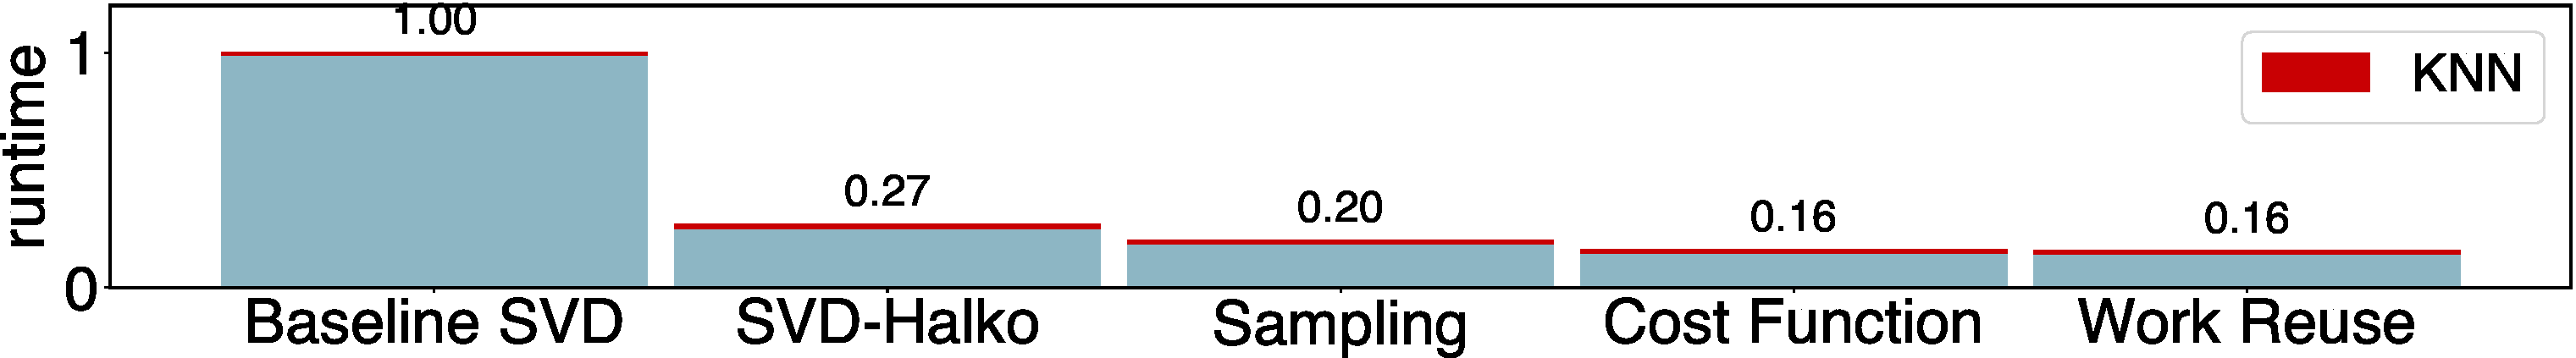
\includegraphics[width=\linewidth]{figs/yoga.pdf} 
     \caption[]{yoga}
     \end{figure} 
     

 \begin{figure}[H]
     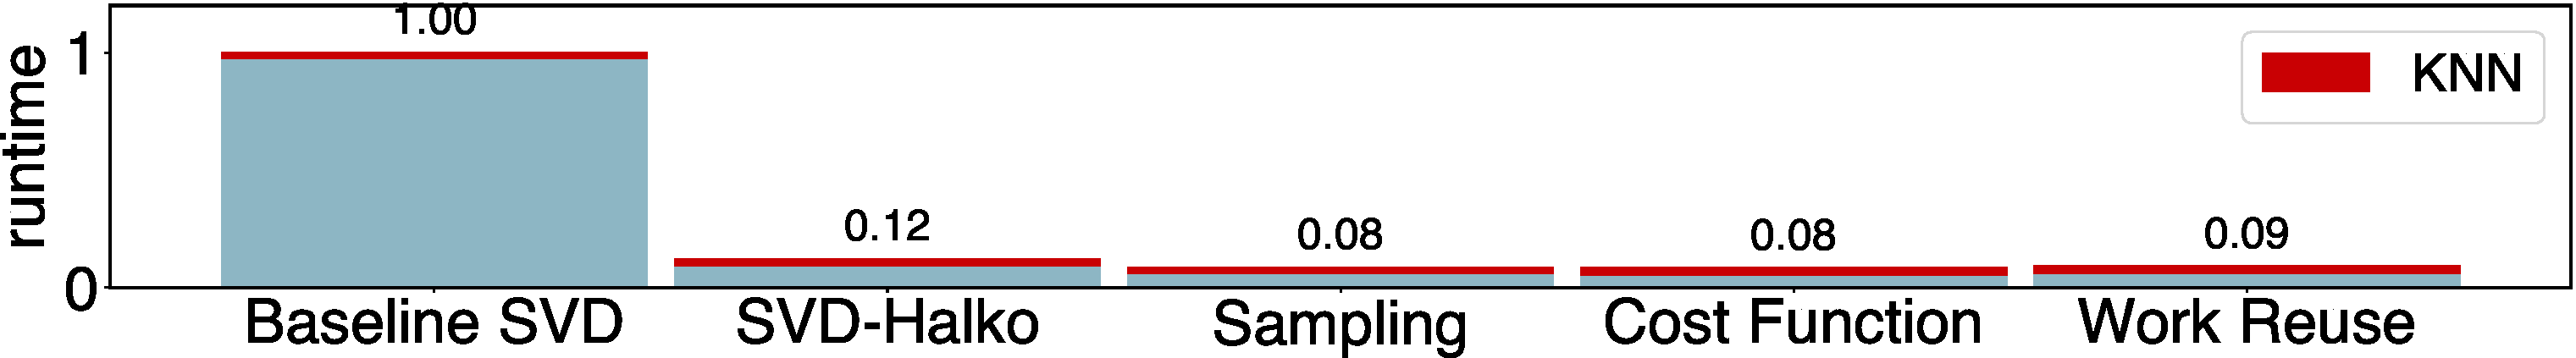
\includegraphics[width=\linewidth]{figs/uWaveGestureLibrary_Y.pdf} 
     \caption[]{uWaveGestureLibrary Y}
     \end{figure} 
     

 \begin{figure}[H] 
     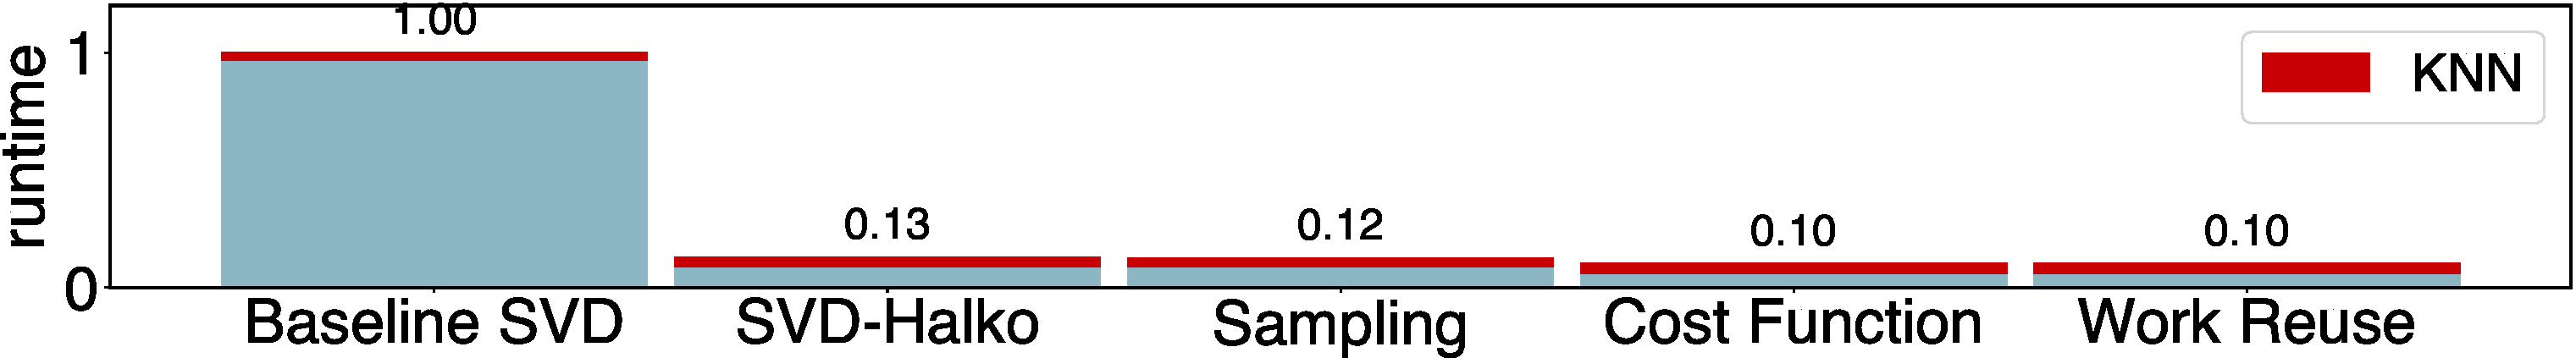
\includegraphics[width=\linewidth]{figs/uWaveGestureLibrary_X.pdf} 
     \caption[]{uWaveGestureLibrary X}
     \end{figure} 
     

 \begin{figure}[H] 
     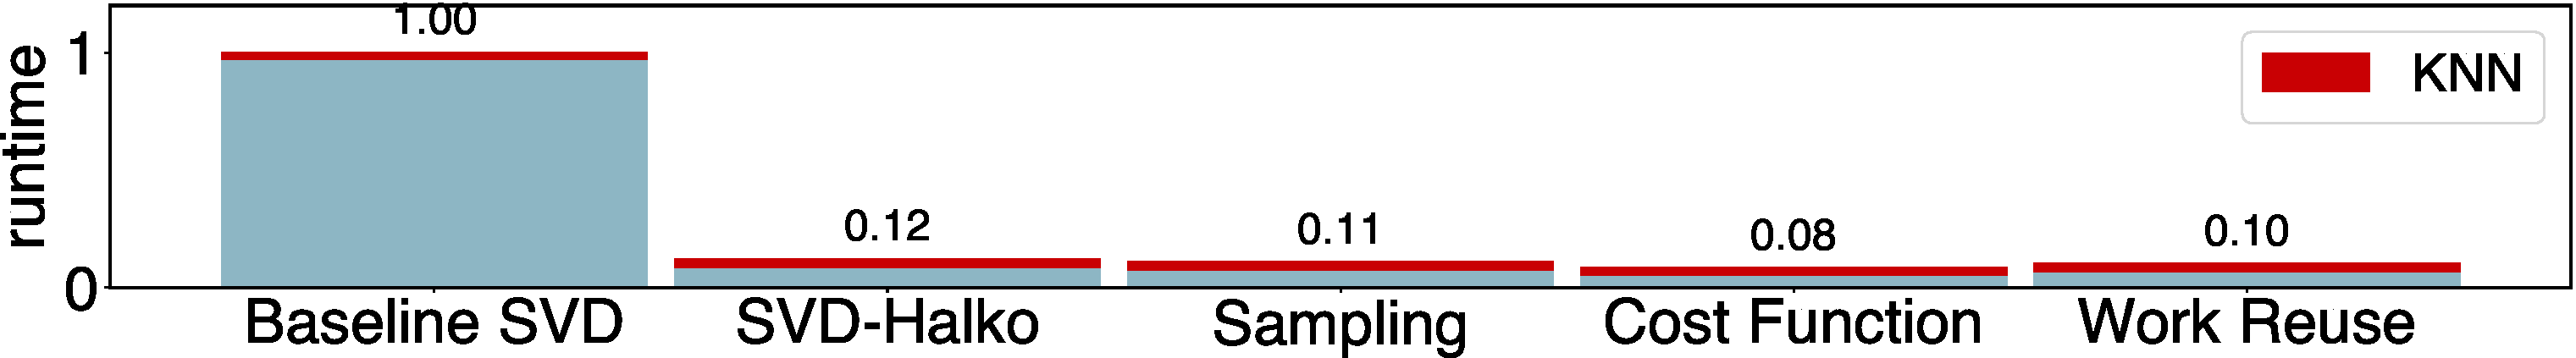
\includegraphics[width=\linewidth]{figs/uWaveGestureLibrary_Z.pdf} 
     \caption[]{uWaveGestureLibrary Z}
     \end{figure} 
     

 \begin{figure}[H] 
     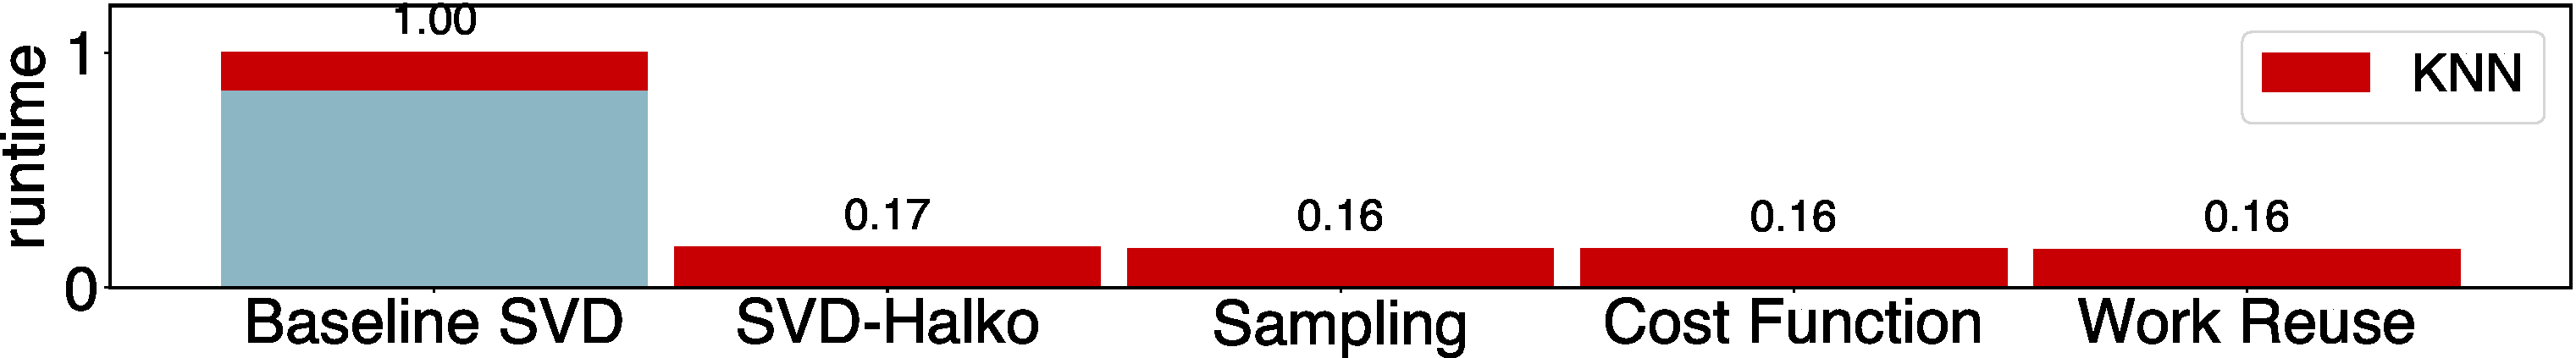
\includegraphics[width=\linewidth]{figs/ElectricDevices.pdf} 
     \caption[]{ElectricDevices}
     \end{figure} 
 
     

 \begin{figure}[H] 
     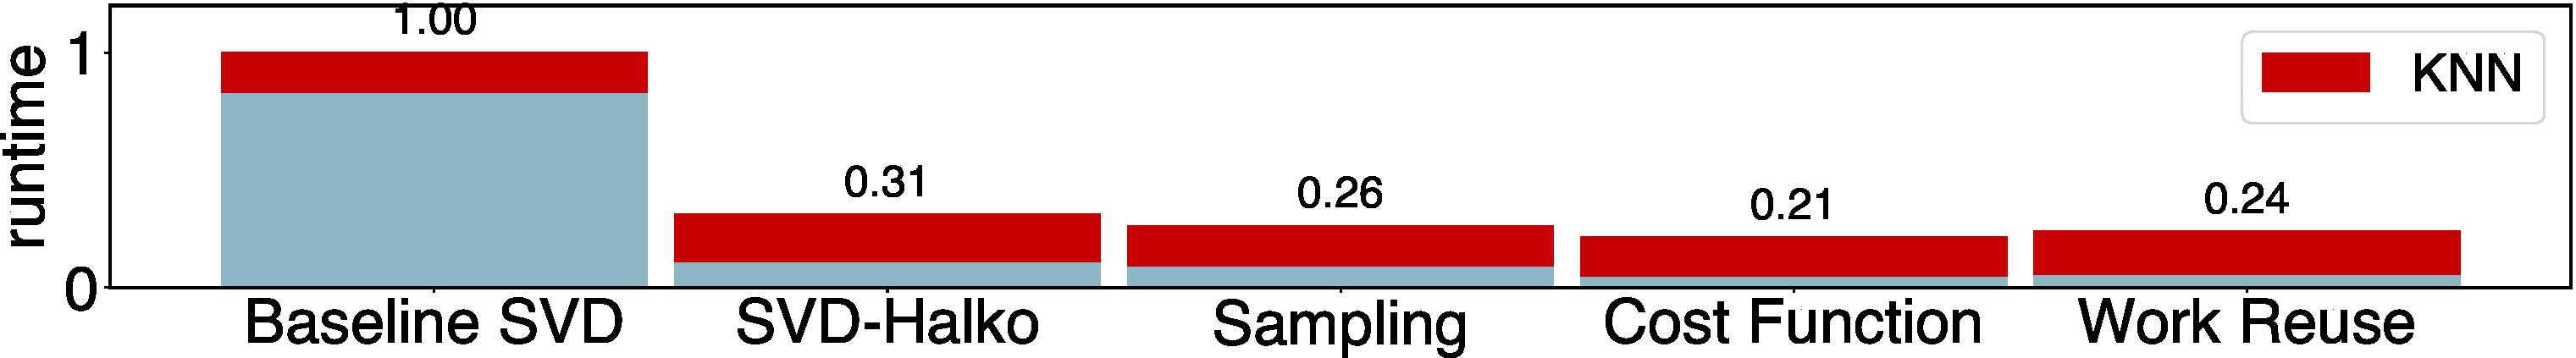
\includegraphics[width=\linewidth]{figs/FordB.pdf} 
     \caption[]{FordB}
     \end{figure} 
     

 \begin{figure}[H] 
     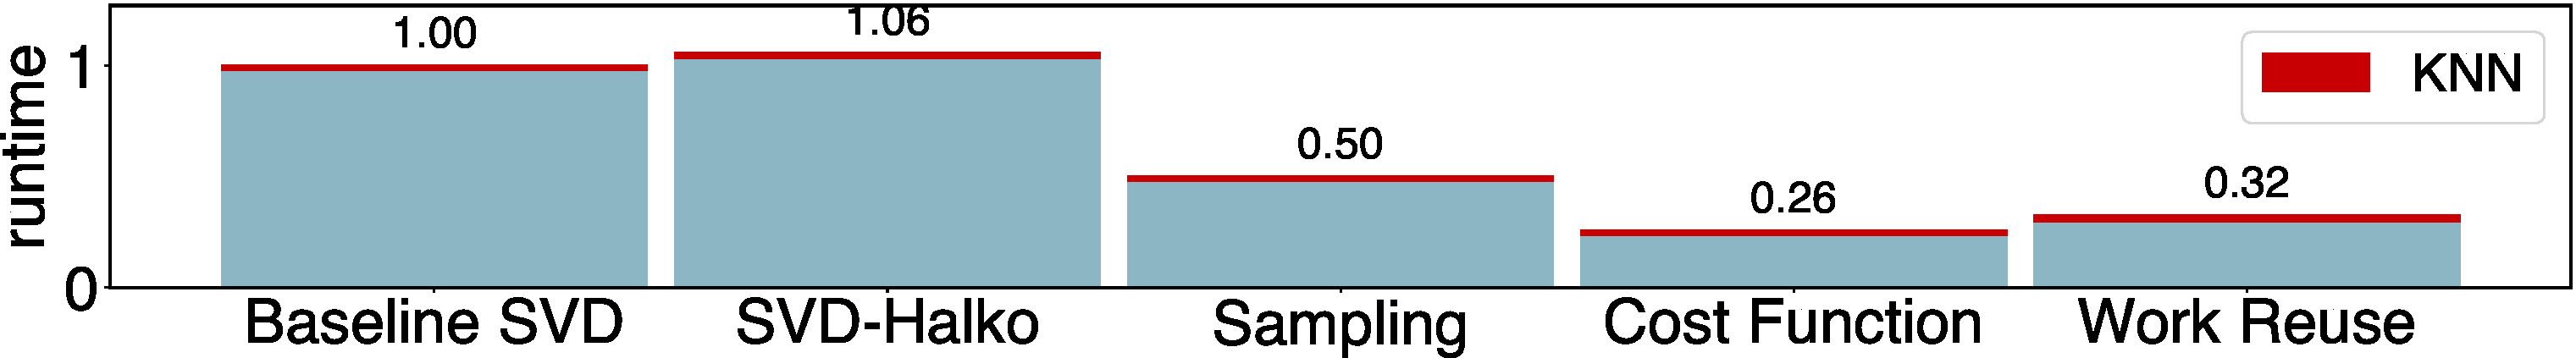
\includegraphics[width=\linewidth]{figs/MALLAT.pdf} 
     \caption[]{MALLAT}
     \end{figure} 
     

 \begin{figure}[H] 
     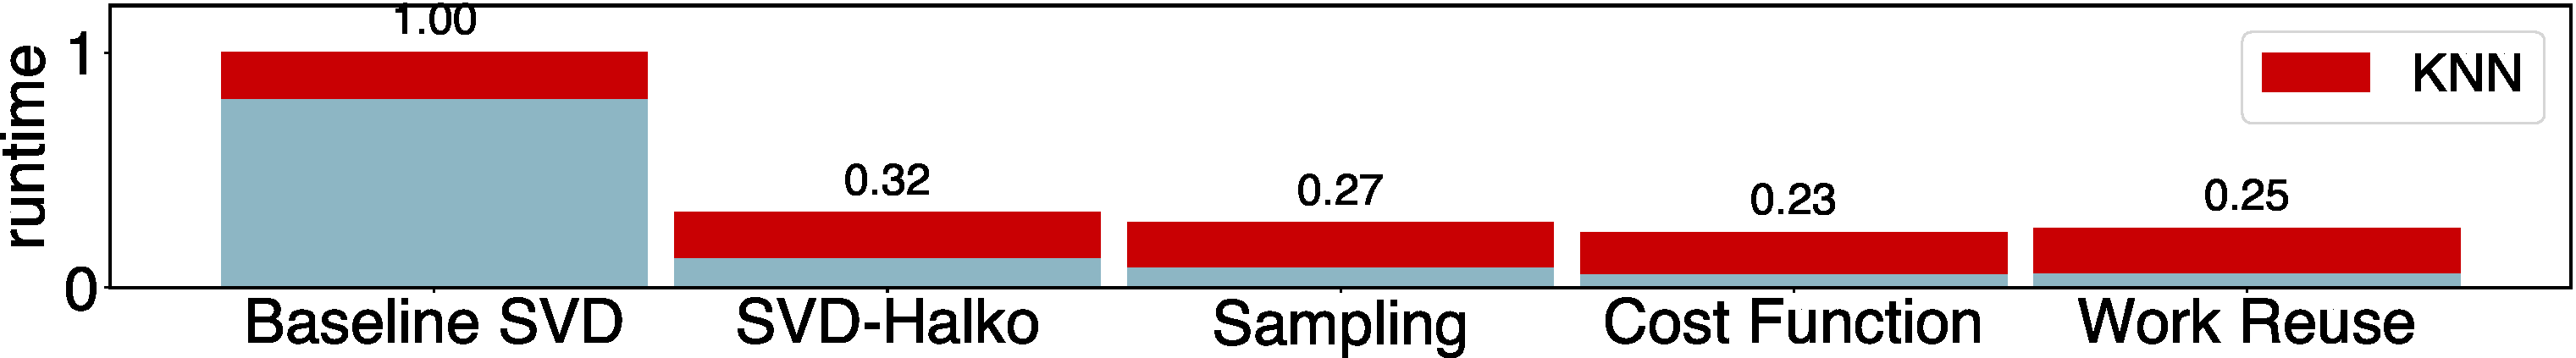
\includegraphics[width=\linewidth]{figs/FordA.pdf} 
     \caption[]{FordA}
     \end{figure} 
     

 \begin{figure}[H] 
     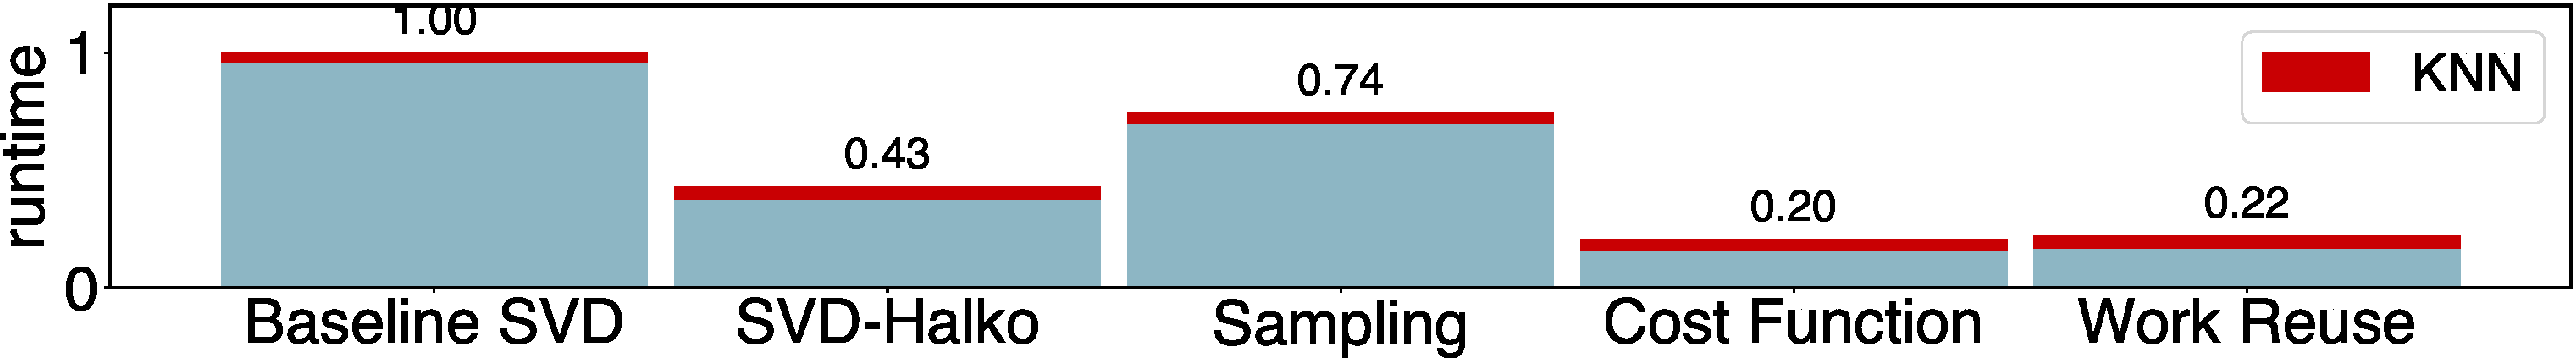
\includegraphics[width=\linewidth]{figs/NonInvasiveFatalECG_Thorax1.pdf} 
     \caption[]{NonInvasiveFatalECG Thorax1}
     \end{figure} 
     

 \begin{figure}[H] 
     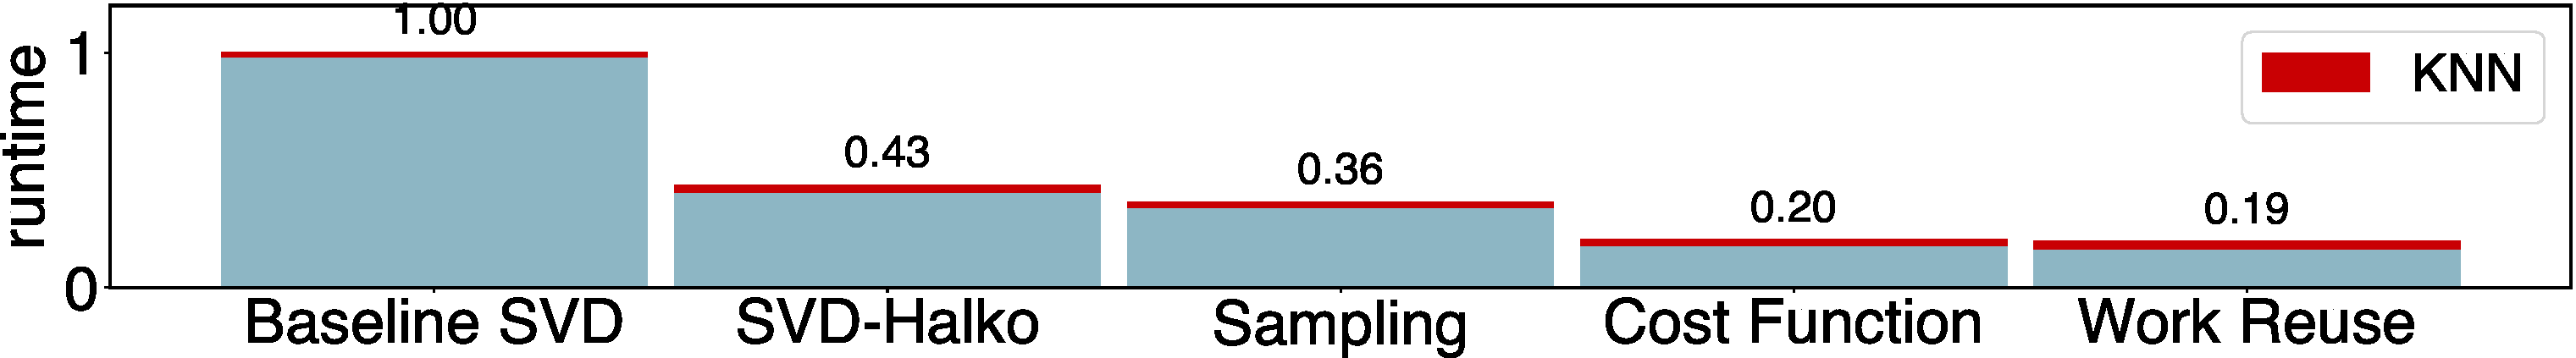
\includegraphics[width=\linewidth]{figs/NonInvasiveFatalECG_Thorax2.pdf} 
     \caption[]{NonInvasiveFatalECG Thorax2}
     \end{figure} 
     

 \begin{figure}[H] 
     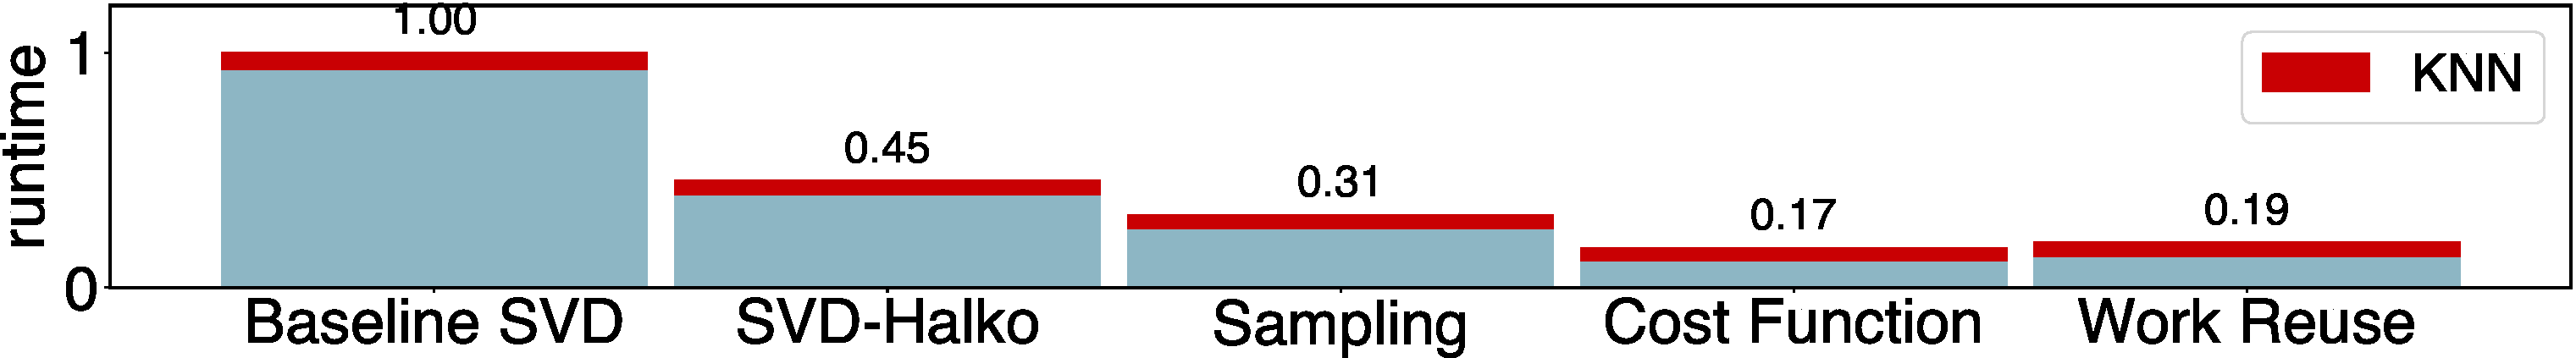
\includegraphics[width=\linewidth]{figs/UWaveGestureLibraryAll.pdf} 
     \caption[]{UWaveGestureLibraryAll}
     \end{figure} 
     

 \begin{figure}[H] 
      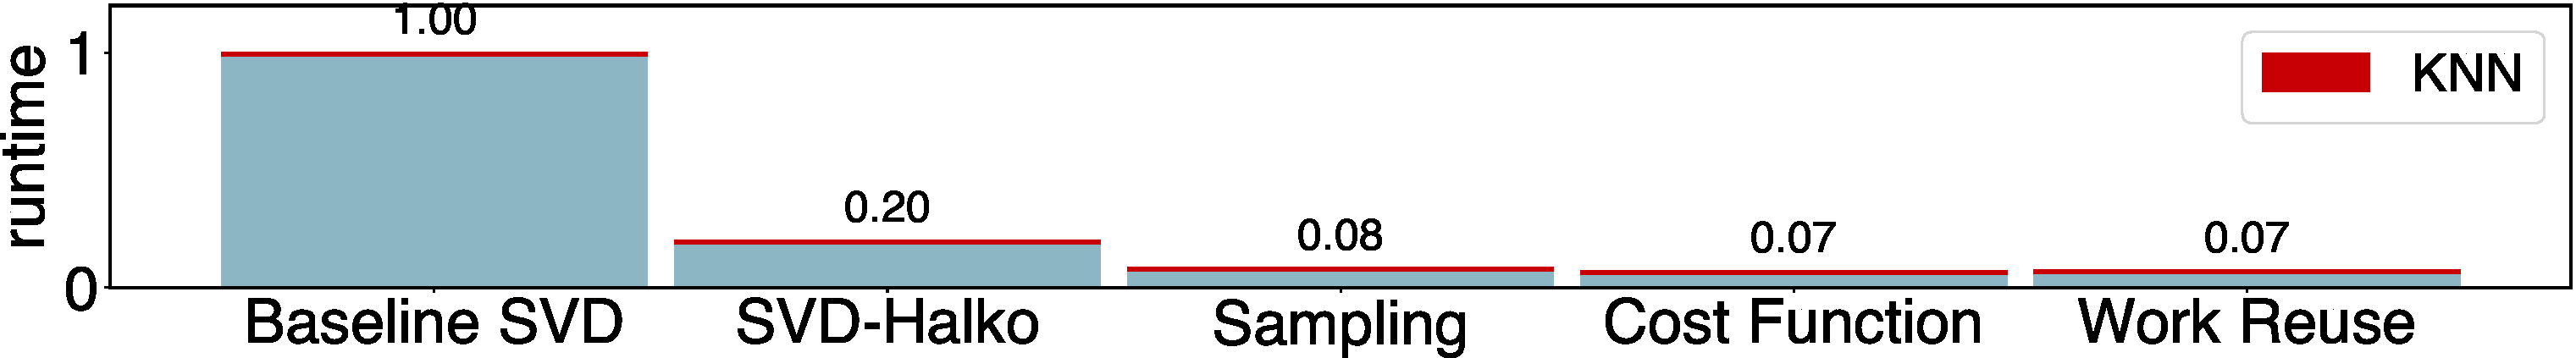
\includegraphics[width=\linewidth]{figs/StarLightCurves.pdf} 
     \caption[]{StarLightCurves}
     \end{figure} 
\end{comment}



%\input{endendplots}

\end{document}
